% LaTeX Datei f�r Projektarbeiten etc. am MZH

% ------------------------------------------------------------------------------------------
% erlaubt das Anfangen des Draft-Modus und damit Ver�nderungen
% einzustellen
\newif\ifdraft
% Draft-Modus: Arbeitsversion, Bilder werden nur als Rahmen dargestellt
% Vorteil: schnelleres Kompilieren
%\drafttrue % <- daf�r hier die Kommentierung wegnehmen

%-------------------------------------------------------------------------------------------
% folgende Befehle sorgen daf�r, das f�r jede Schrift die richtigen Pakete installiert werden
\newcounter{schrift}
% Schrift ausw�hlen:
% 1 - mathptmx
% 2 - minionpro
% 3 - mathpazo
% 4 - times + computer modern
% 5 - computer modern
\setcounter{schrift}{4} % Hier die entsprechende Zahl setzen !

% ------------------------------------------------------------------------------------------
% ------------------------------------------------------------------------------------------
% Latex - Pr�ambel
% hier werden alle wichtigen Dokumenteinstellungen getroffen, normalerweise m�ssen
% keine �nderungen mehr durchgef�hrt werden.
% Pakete die das Schriftbild, den Satzspiegel oder die R�nder ver�ndern, d�rfen
% nicht hinzugef�gt werden, erst nach Abstimmung mit dem Betreuer.
% n�tzliche Pakete sind willkommen, bitte die Wiki entsprechend aktualisieren
% viele Pakete sind drin, die vielleicht nicht jeder braucht und das Kompilieren verl�ngern
% sollten diese das Layout nicht ver�ndern, k�nnen diese nat�rlich auskommentiert werden.
% ------------------------------------------------------------------------------------------

% ------------------------------------------------------------------------------------------
% Dokumentenklasse definieren:
\ifdraft
    \documentclass[draft, 
                   paper=a4,
                   xcolor=dvipsnames,
                   BCOR5mm,
                   fontsize=12pt, 
                   DIV13, 
                   headsepline, 
                   numbers=noenddot, 
                   %bibtotoc,
                   bibliography = totoc,
                   %version=first,
                   %smallheadings,
                   headings = small,
                   oneside]{scrbook}
\else
    \documentclass[paper=
                   a4,
                   xcolor=dvipsnames,
                   BCOR5mm,
                   fontsize=12pt, 
                   DIV13, 
                   headsepline, 
                   numbers=noenddot, 
                   %bibtotoc,
                   bibliography = totoc, 
                   %version=first,
                   %smallheadings,
                   headings = small,
                   headinclude=true,
                   footinclude=false,
                   fleqn, % formeln links b�ndig
                   oneside]{scrbook}
\fi
% Standard-Koma-Dokument mit
%   Papierformat A4
%   Binderand 5 mm
%   Schrift 12-Punkt
%   Seitenlayout nach DIV, siehe scrguide.pdf text b/h rand oben/innen: 168,00 237,60 19,80 14,00 (ist raus)
%   Linie unter der Kopfzeile
%   Nummern ohne Punkt am Ende
%   Literaturverzeichnis im Inhaltsverzeichnis
%   �berschriften etwas kleiner als standard
%   weitere Informationen zum Koma-Skript: www.komascript.de

%---------------------------------------------------------------
% Basis-Pakete
%---------------------------------------------------------------
\usepackage{ifpdf}		%   Ueberprueft, ob LaTeX oder pdfLaTeX verwendet wird (nur ab MikTeX 2.5)
\usepackage[T1]{fontenc}        %   8-Bit-Fonts
\usepackage{textcomp,latexsym}  %   zusaetzliche Symbole
\usepackage[utf8]{inputenc}   %   Quelltext ist Latin-1 (d.h. Windows-) kodiert
\usepackage[ngerman]{babel}            %   neue deutsche Rechtschreibung
\usepackage{scrtime}            %   fuer die aktuelle Zeit
%\usepackage{scrdate}            %   fuer das aktuelle Datum
%\usepackage{natbib}             %   Literaturverweise mit (Autor Jahr) nach DIN
%\bibpunct[; ]{[}{]}{,}{a}{}{;}  %   eckige Klammern statt runde bei Zitaten
%\usepackage[T1]{url}            %   Web-Addressen auch mit T1-Encoding
%\urlstyle{tt}                   %   und in tt-Font
%\usepackage[activate=normal]{pdfcprot} % dient dem optischen Randausgleich bei k�rzeren Zeichen wie '-', '.', ',', '!'

\usepackage{color}

\PassOptionsToPackage{x11names}{xcolor}
\usepackage[dvipsnames]{xcolor}


%---------------------------------------------------------------
% n�tzliche Zusatz-Pakete
%---------------------------------------------------------------
%\usepackage{makeidx}            %   Index (wenn gewuenscht)

\usepackage{setspace}           %   Zeilenabstand setzen. Befehl:
                                %   \begin{spacing{Wert}
                                %   Text
                                %   \end{spacing}
%\usepackage{placeins}           %   das Positionieren von float-Umgebungen bestimmen:
                                %   der Befehl \floatbarrier sorgt daf�r, dass alle vorher eingegebenen
                                %   float-Umgebungen VOR diesem Befehl eingef�gt werden.
                                
%\usepackage{subfig}          %   Bilder gruppieren, mehrere Bilder in einer Umgebung einf�gen
                                %   Bsp.:
                                %   \begin{figure}
                                %   \centering
                                %    \subfloat[Text a]
                                %    {\includegraphics{bild a}}
                                %    \subfloat[text b]
                                %    {\includegraphics{bild b}}
                                %    \caption{Untertitel}
                                %    \label{fig.Beziechnung_subfigure} <- am besten mit fig. dann kann mit \bild{Bezeichnung_figure} referenziert werden
                                %   \end{figure}                                

%\usepackage{textcomp}           %   fuer Trademark und Copyright Zeichen
                                %   z.B \texttrademark, \textregistered, \texteuro etc.

\usepackage{tabularx}           %   erweiterte Funktionen f�r Tabellen

\usepackage{tabularx}           %   erwieterte Funktionen f�r Tabellen

\usepackage{longtable}          %   Longtable-Package f�r Tabellen die l�nger als eine DIN-A4-Seite sind

\usepackage{colortbl}						%		farbige Tabellenzeilen

\usepackage{nicefrac}           %   Schr�ge Bruchstriche \nicefrac{Nenner}{Z�hler}

%\usepackage{numprint}           %   Zahlen mit Einheiten n�her an der Zahl/kein Umbruch und 1 000er Format \numprint[Einheit]{Zahl}

%\usepackage{mathcomp}           %   f�r \tcdegree (� Gradzeichen bei numprint) \numprint[\tcdegree]{180} f�r 180�

%\usepackage{hhline}             %   hhline-Package
                                %   Fuer komplexe Linienzuege in Tabellen \hhline{}
                                %   = Spalte mit doppelter Linie      | vertikale Linie die horizontale schneidet
                                %   - Spalte mit einfacher Linie      : vertikale Linie die von horizantaler unterbrochen ist
                                %   ~ Spalte ohne Linie               # doppelte horiz. geschnitten mit doppelter vert. Linie
                                %   t oberer Teil ->                  b unterer Teil einer doppelten Linie

%\usepackage[active]{srcltx}     %   bei verwendung v. \includeonly spring winedt jetzt bei fehlern an die richtige stelle

\usepackage{flafter}            %   Ein float-Objekt immer erst NACH seiner Definition platzieren

\usepackage{ifthen}             %   definiert \ifthenelse{}{}{}

%\usepackage{path}               %   dateinamen und pfade darstellen

%\usepackage{pdfsync}						%   Synchronisation mit SumatraPDF <<-- geht auch ohne

\usepackage{booktabs}

%% Eigene Pakete

\usepackage{scrhack} % L�scht Warnungen von Packages wie hyperref, listings
\usepackage[ locale = DE,            % deutsch
            load-configurations=abbreviations, % zus�tzliche Einheiten siehe manual
            per-mode=symbol,%-or-fraction,
            separate-uncertainty% 
            ]
            {siunitx}								% SI-Einheiten  

            
\usepackage{multirow}               % zwei Zeilen kombinieren (wie multicolumn)
\usepackage[babel]{microtype}       % schickeres Schriftbild -> aber l�ngeres Kompilieren

\usepackage{blindtext}							% sinnlosen text einbauen
\usepackage{subfigure}

\usepackage{newunicodechar}

%\usepackage{slashbox}
\usepackage{rotating}
\usepackage{pdflscape}

\usepackage{algorithm}
\usepackage{algpseudocode}

\usepackage{eqparbox}
\renewcommand\algorithmiccomment[1]{%
  \hfill$\triangleright$\ \eqparbox{COMMENT}{#1}%
}
\newcommand\LONGCOMMENT[1]{%
  \hfill$\triangleright$\ \begin{minipage}[t]{\eqboxwidth{COMMENT}}#1\strut\end{minipage}%
}


%\newunicodechar{ }{~}

%\DeclareUnicodeCharacter{00A0}{~}


%%

%---------------------------------------------------------------
% Grafik-Paket f�r eps bzw. pdf
%---------------------------------------------------------------
% �berpr�ft ob Latex oder PDFLatex ausgef�hrt wird, dementsprechend werden pdf/jpg oder eps Bilder eingef�gt
% sollen dvi oder pdf Dokumente erstellt werden m�ssen alle Bilder in beiden Formaten vorliegen
% hierf�r gibt es Tools wie epstopdf oder jpgtoeps
 \ifdraft
    \usepackage[draft]{graphicx}
\else
    \ifpdf
        \usepackage{graphicx}
        \usepackage{pgfplots} % pgfplots zum plotten in LaTeX
    \else
        \usepackage[final]{graphicx}
    \fi
\fi
% von wo sollen die Grafiken kommen?
\graphicspath{{./fotos/}{./skizzen/}{./zeichnungen/}}

\usetikzlibrary{pgfplots.statistics}

%Einstellungen f�r pgfplots
\pgfplotsset{compat=1.8,
	%enlargelimits=auto,
	tick label style={font=\small,/pgf/number format/use comma}, %Komma nutzen in allen Axen
	%axis x line=center, %alle x-Achsen center
	%axis y line=center, %alle y-achsen center
	%every axis x label/.style={at={(current axis.right of origin)},anchor=west}, % achsenbeschriftung bei allen x-achsen rechts
	%every axis y label/.style={at={(current axis.above origin)},anchor=south},   % achsenbeschriftung bei allen y-achsen oben
	%every x tick scale label/.style={at={(current axis.right of origin)},anchor=north,yshift=-0.5em}, %positionierung des scale faktors ge�ndert
	every axis legend/.append style={at={(0.5,1.03)},anchor=south,nodes=right,font=\small}, % Legende �ber der Grafik, schriftgr��e small
	label style={font=\small} % label schriftgr��e small
}
\newlength\tikzwidth
\setlength{\tikzwidth}{0.7\textwidth}
\definecolor{mycolor1}{rgb}{0,0.5,0}

\ifpdf
 \ifdraft
    \usepackage[draft]{pdfpages}%   externe PDF Seiten einbinden nur bei PDF-Latex m�glich
    \else
    \usepackage[final]{pdfpages}%   externe PDF Seiten einbinden nur bei PDF-Latex m�glich
 \fi                            %   Befehl: \includepdf{PDF-Datei} soll die Datei im Querformat angezeigt werden
    \else
\fi                             %   \includepdf[landscape=true]{PDF-Datei}

%---------------------------------------------------------------
% Debug-Ausgabe der Labels und References
%---------------------------------------------------------------
\ifdraft
  \usepackage{showkeys} % Label werden im Draft Modus im Text angezeigt
\fi

%---------------------------------------------------------------
% Abweichende PostScript-Schriftarten
% werden in der main Datei ausgew�hlt, hier nichts �ndern
%---------------------------------------------------------------
\ifthenelse{\equal{ 1 }{ \value{schrift} }}
    {
    \usepackage{mathptmx}          %   Times als Hauptschriftart, keine mathematische Fettschrift
    \usepackage{amssymb}
    \usepackage{amsbsy}
    \usepackage{amsmath}
    \usepackage{amsfonts}
    \usepackage{amstext}
    \renewcommand{\boldsymbol}[1]{\mathbf{#1}} % nur bei mathptmx !
                                               % damit boldsymbol wenigstens fette aufrechte Buchstaben macht
    }{}
\ifthenelse{\equal{ 2 }{ \value{schrift} }}
    {
    \usepackage[lf, minionint]{MinionPro} %   OpenType von Adobe, mathematische Fettschrift vorhanden, Schrift ist
                                %   ist im Standard-LaTeX nicht installiert.
                                %   Ist ein wenig Aufwand das Ganze zu installieren, Matthias Dagen fragen
    }{}
\ifthenelse{\equal{ 3 }{ \value{schrift} }}
    {
    \usepackage{mathpazo}          %   nette Buchschrift aber sehr gross, mathematische Fettschrift vorhanden
    \usepackage{amssymb}
    \usepackage{amsbsy}
    \usepackage{amsmath}
    \usepackage{amsfonts}
    \usepackage{amstext}
    }{}
\ifthenelse{\equal{ 4 }{ \value{schrift} }}
    {
    \usepackage{times}
    \usepackage{amssymb}
    \usepackage{amsbsy}
    \usepackage{amsmath}
    \usepackage{amsfonts}
    \usepackage{amstext}
    }{}
\ifthenelse{\equal{ 5 }{ \value{schrift} }}
    {
    \usepackage{amssymb}
    \usepackage{amsbsy}
    \usepackage{amsmath}
    \usepackage{amsfonts}
    \usepackage{amstext}
    \usepackage{lmodern}
    }{}
\usepackage[scaled=.92]{helvet} %   11pt Helvetica f�r �berschriften etc. etwas kleiner da, Helvetica an sich gr��er ist
%\usepackage{courier}            %   Courier bei \texttt
%\usepackage{upgreek}            %   Aufrechte griechische Buchstaben

% ------------------------------------------------------------------------------------------
% Bild- und Tabellentitel FETT
% ------------------------------------------------------------------------------------------
%\def\figurename{\bfseries Bild}
%\def\tablename{\bfseries Tabelle}

%%Andere Beschreibung von figure
\addto\captionsngerman{
	\renewcommand{\figurename}{\bfseries Bild}%%Andere Beschreibung von figure
	\renewcommand{\listfigurename}{Bildverzeichnis}
	\renewcommand{\tablename}{\bfseries Tabelle}
}

%---------------------------------------------------------------
% Quelltexte formatieren
%---------------------------------------------------------------
\usepackage{listings}


%\lstloadlanguages{
		%C,
		%C++,
		%XML
%}

\lstset{
		language=XML,
		basicstyle=\footnotesize\ttfamily, % Standardschrift
		numbers=left,               % Ort der Zeilennummern
		numberstyle=\tiny,          % Stil der Zeilennummern
		numbersep=5pt,              % Abstand der Nummern zum Text
		tabsize=2,                  % Groesse von Tabs
		extendedchars=true,         %
		breaklines=true,            % Zeilen werden Umgebrochen        
		keywordstyle=\color{Red2},
		frame= b,         
		stringstyle=\color{Purple2}\ttfamily, % Farbe der String
		showspaces=false,           % Leerzeichen anzeigen ?
		showtabs=false,             % Tabs anzeigen ?
		xleftmargin=17.5pt,
		framexleftmargin=17pt,
		framexrightmargin=5pt,
		framexbottommargin=4pt,
		linewidth= \dimexpr\textwidth-2\fboxsep-2\fboxrule,
		comment=[l]{\#},
		morecomment=[s]{<!--}{-->},
		commentstyle=\color{Green4},
		%backgroundcolor=\color{grey},
		showstringspaces=false,      % Leerzeichen in Strings anzeigen ?        
		morekeywords={__global__, name, pkg, args, type, from, to, textfile, respawn, value, output, radius, ixx, ixy, ixz, iyy, iyz, xyz, rpy, reference},  % CUDA specific keywords
		aboveskip = 18pt, 
		belowskip = 18pt
}

\usepackage{caption}
\DeclareCaptionFont{white}{\color{white}}
\DeclareCaptionFormat{listing}{\colorbox{darkgray}{\parbox{\dimexpr\textwidth-2\fboxsep-2\fboxrule}{\hspace{15pt}#1#2#3}}}
\captionsetup[lstlisting]{format=listing,labelfont=white,textfont=white, singlelinecheck=false, margin=0pt, font={bf,footnotesize}}

%---------------------------------------------------------------
% ein paar L�ngen einstellen
%---------------------------------------------------------------
%\setlength{\parskip}{1ex plus0.5ex minus0.2ex} % Absatzabstand etwas gr��er
\setlength{\itemsep}{0ex plus0.2ex}            % Abstand zweier Listenelemente kleiner
\setlength{\parindent}{0ex}                     % kein Absatzeinzug
\setlength{\belowcaptionskip}{0.4cm}            % Abstand caption - Tabelle gr��er
\setlength{\abovecaptionskip}{0.4cm}            % Abstand caption - Tabelle gr��er

%---------------------------------------------------------------
% Kopf- und Fusszeilen
%---------------------------------------------------------------
\usepackage[plainheadsepline,  % linie zw. kopf und text auch bei seitenstil "plain"
           %headexclude,       % kopfzeile geh�rt nicht zum textk�rper
           %footexclude        % fusszeile geh�rt nicht zum textk�rper
          ]       
           {scrpage2}
\pagestyle{scrheadings}
\clearscrheadfoot              % voreinstellungen loeschen
\ihead{\normalfont\headmark}   % kolumnentitel innen
\ohead[\pagemark]{\pagemark}   % seitenzahl aussen

%---------------------------------------------------------------
% Nummerierungs-Tiefe des Inhaltsverzeichnis und der Abschnitte einstellen
%---------------------------------------------------------------
\setcounter{secnumdepth}{2} \setcounter{tocdepth}{2}

%---------------------------------------------------------------
% Abk�rzungsverzeichnis
%---------------------------------------------------------------
% mit dem Befehl \nomenclature[l/g/a]{Abk�rzung}{Bezeichnung} kann direkt im Code die Abk�rzung eingef�gt werden
% das Paket sortiert diese und f�gt sie mit dem Befehl \printnomenclature ein
% l, g, oder a steht dabei f�r die Gruppierung Lateinische bzw. Griechische Buchstaben, Abk�rzungen
% Nach Einf�gen neuer Abk�rzungen muss folgender Befehl in der Eingabeaufforderung im Tex-Verzeichnis eingegeben werden:
% -> vorher einmal kompilieren
% -> makeindex main.nlo -s nomencl.ist -o main.nls
% -> nochmal kompilieren
%\makeindex
\usepackage{nomencl}
% \let\abbrev\nomenclature
\renewcommand{\nomname}{Abk�rzungsverzeichnis}
\setlength{\nomlabelwidth}{.25\hsize}
\renewcommand{\nomlabel}[1]{#1 \hfill}
\setlength{\nomitemsep}{-\parsep}

\renewcommand{\nomgroup}[1]{%
	\ifthenelse{\equal{#1}{L}}{\item[\textbf{Lateinische Buchstaben}]}
	{%
		\ifthenelse{\equal{#1}{G}}{\item[\textbf{Griechische Buchstaben}]}
		{%
			\ifthenelse{\equal{#1}{A}}{\item[\textbf{Abk�rzungen}]}
			{
				\ifthenelse{\equal{#1}{K}}{\item[\textbf{Koordinatensysteme}]}{}
			}
		}
	}
}

\makenomenclature

%---------------------------------------------------------------
% Hyperlinks f�r pdfTeX
%---------------------------------------------------------------
\ifpdf
    % hier stehen befehle, die nur f�r pdftex gelten
    \usepackage[pdfpagelabels,  % logische (z.b. auch roemische) seitenzahlen
                bookmarks,       % Bookmarks f�r die einzelnen Abschnitte
                pdftex
                ]{hyperref}
    \hypersetup{
    %   colorlinks,  % Links mit farbigem Text
        pdfborder   = 0 0 0,
        plainpages  = false,
        bookmarksnumbered = true,
    %   bookmarksopen
    }
\else
    % hier stehen befehle, die nur f�r latex gelten
    \usepackage{hyperref} % hier ohne colorlinks und pdf-krams
\fi

%extra inhaltsverzeichnisse m�glich
\usepackage[nohints]{minitoc}     
\renewcommand{\mtctitle}{Anhangsverzeichnis} 				% Name �ndern            
\renewcommand{\mtifont}{\large\bfseries\sffamily}		% Titel font �ndern
\renewcommand{\mtcSfont}{\rm}												% Section eintr�ge normal
\mtcsetrules{minitoc}{off}													% Linien ausmachen

%---------------------------------------------------------------
% SVGs einf�gen
%---------------------------------------------------------------
%% SVG to TeX
% from InkscapePDFLaTeX.pdf
% by Johan Engelen, 2010
% Information: 
% http://tug.ctan.org/tex-archive/info/svg-inkscape
% -shell-escape muss im Ausgabeprofil stehen
% inkscape.exe muss im Path-Folder sein

% Funktion zum ueberpruefen auf Aenderung
\newcommand{\executeiffilenewer}[3]{%
                \ifnum\pdfstrcmp{\pdffilemoddate{#1}}%
                {\pdffilemoddate{#2}}>0%
                {\immediate\write18{#3}}\fi%
}
% Wenn Aenderung dann TeX-Export ausfuehren und einbinden
%\newcommand{\includesvg}[1]{%
                %\executeiffilenewer{#1.svg}{#1.pdf}%
                %{inkscape -z -C --file=#1.svg %
                %--export-pdf=#1.pdf --export-latex}%
                %\input{#1.pdf_tex}%
%}

% set inkscape binary path according to operating-system
\IfFileExists{/dev/null}{%
  \newcommand{\Inkscape}{inkscape }%
  }{%
  \newcommand{\Inkscape}{"C:/Program Files (x86)/Inkscape/inkscape.exe" }%
}
% includesvg[scale]{file} command
\newcommand{\includesvgnew}[2][1]{%
  \executeiffilenewer{#2.svg}{#2.pdf}{%
  \Inkscape -z -D --file="#2.svg" --export-pdf="#2.pdf" --export-latex}%
  \scalebox{#1}{\input{#2.pdf_tex}}%
}

%% Include svg mit Text aus textext plugin
% text wird im svg mit textext hinzugef�gt.
% falls �nderungen im .svg gefunden werden, wird das Bild 
% neu exportiert und eingef�gt.
% \includesvg{ordner/file} /ohne endung
\newcommand{\includesvg}[4][]{
			\executeiffilenewer{#3.svg}{#3.pdf}
			{inkscape -z -D --file=#3.svg
			--export-pdf=#3.pdf}
			\begin{figure}[#2]
				\centering
				\includegraphics[#1]{#3}
				\caption{#4} \label{fig.#3}
				\vspace*{-3mm}
			\end{figure}
}

\newcommand{\includesinglesvg}[2][]{
			\executeiffilenewer{#2.svg}{#2.pdf}
			{inkscape -z -D --file=#2.svg
			--export-pdf=#2.pdf}
			\includegraphics[#1]{#2}
}

\usepackage[right]{eurosym}

\usepackage{chngcntr}						%Added by LC, consistent numbering of footnotes throughout whole document
\counterwithout{footnote}{chapter}			%Added by LC


%für die Gliederung
\let\Contentsline\contentsline 
\renewcommand\contentsline[3]{\Contentsline{#1}{#2}{}}
\makeatletter
\renewcommand{\@dotsep}{10000} 
\makeatother                           % Pr�ambel zur Dokumentenformatierung einf�gen
                                            % braucht nicht zu ver�ndert werden, stehen aber n�tzliche
                                            % Hinweise drin

%---------------------------------------------------------------
% Trennmuster fuer Ausnahmef�lle
%---------------------------------------------------------------
\hyphenation{} % z.B. \hypenation{Trenn-text}

%---------------------------------------------------------------
% Dokumentenanfang:
%---------------------------------------------------------------
% Einstellungen f�r PDF-Latex:
% Hier Titel etc. eintragen, dann wird es in den Dokumenteneigenschaften vom PDF richtig angezeigt
\ifpdf
    \hypersetup{
    %   colorlinks,  % Links mit farbigem Text
        pdftitle    = {Titel},
        pdfsubject  = {Diplomarbeit},
        pdfauthor   = {Lennart Claassen},
        pdfkeywords = {}
        }
\else
\fi

\usepackage{befehle}                        % eigene Befehle wie:
                                            % \zB\,
                                            % \abbildung{Position h,b,t,p}{Dateiname ohne Endung}{Caption}
                                            % \bild{Dateiname}, referenziert gem�� ...Bild x.xx...
                                            % einfach mal nachschauen was so drin ist und eigene Befehle f�r
                                            % wiederholende Sachen definieren

%\includeonly{ergebnisse}                   % wenn nur ein Kapitel kompilliert werden soll
                                            % geht schneller wenn man nur das Layout des Kapitels sehen will

%\entwurf                                   % Entwurfsdatum auf jede Seite setzen,
                                            % nicht vergessen beim Druck rauszunehmen
%\setlength\overfullrule{5pt}                % Overfull boxes werden angezeigt
%\setlength\underfullrule{5pt} 

% Seitenspiegel neu berechnen
\typearea[current]{last}
%\typearea{last}

\def\TReg{\textsuperscript{\textregistered}}	%Added by LC Copyright symbols etc.
\def\TCop{\textsuperscript{\textcopyright}}
\def\TTra{\textsuperscript{\texttrademark}}
\newcommand{\mLocalization}{Modul \textbf{Lokalisation} }
\newcommand{\mEkf}{Modul \textbf{Tracking} }
\newcommand{\mFovis}{Modul \textbf{Visuelle Odometrie} }
\newcommand{\mImu}{Modul \textbf{IMU} }
\newcommand{\mVisualization}{Modul \textbf{Visualisierung} }
\newcommand{\mTransformation}{Modul \textbf{Transformation} }
\newcommand{\mInteraction}{Modul \textbf{Interaktion} }
\newcommand{\mGui}{Modul \textbf{Benutzeroberfläche} }
\newcommand{\mProjection}{Modul \textbf{Projektion} }
\newcommand{\mMapserver}{Modul \textbf{Kartenserver} }

\newcommand{\red}[1][TODO]{\textbf{\color{red}{#1}}}

%\newcommand{\pt}[1][p]{$\boldsymbol{#1}$ }
\newcommand{\pt}[1][p]{\ensuremath{
	{\boldsymbol{#1} } 
}}
\newcommand{\pteq}[2][p]{\ensuremath{
	{\boldsymbol{#1} = \left[ {#2} \right] ^T}
}}

%\newcommand{\pti}[2][p]{\ensuremath{
%	{_{(#2)}\boldsymbol{#1} } 
%}}

\newcommand{\pth}[1][p]{\ensuremath{
	{\boldsymbol{\tilde{#1}} }
}}
\newcommand{\ptheq}[2][p]{\ensuremath{
	{\boldsymbol{\tilde{#1}} = \left[ {#2},1 \right] ^T}
}}

%\newcommand{\tran}[3][T]{\ensuremath{
%	{^{#2}\boldsymbol{#1}_{#3} } 
%}}

\newcommand{\kps}[1][]{Kamera-Projektor-System{#1}}


\begin{document}                            % Dokumentenanfang
\dominitoc
\begin{spacing}{1.15}                       % Zeilenabstand auf 1,15 fach stellen, ist nicht so eng aber
                                            % auch nicht so eine Seitenschinderei wie 1,5-fach
    \frontmatter                            % mit kleinen r�mischen Seitenzahlen beginnen f�r class scrbook
    %\pagenumbering{roman}                  % das gleiche f�crartcl
    \setcounter{page}{0}
    \pdfbookmark[0]{Titel}{tit}             % damit der Titel auch im Acrobat angezeigt wird
		\begin{titlepage}
\begin{spacing}{2}

\begin{flushright} %rechtsb�ndig (Anfang)
	\vspace*{-20mm}
	
\includegraphics[width=\textwidth]{CoverLogos}
\end{flushright} %rechtsb�ndig (Anfang)

% der Titel der Arbeit:
\vspace{38mm} {\centering {{\LARGE{Selbstlokalisation eines handführbaren Projektionssystems zur interaktiven Darstellung visueller Zusatzinformationen}}}

\vfill
\vspace{3mm}
% hier kommt ne h�bsche Grafik hin:
%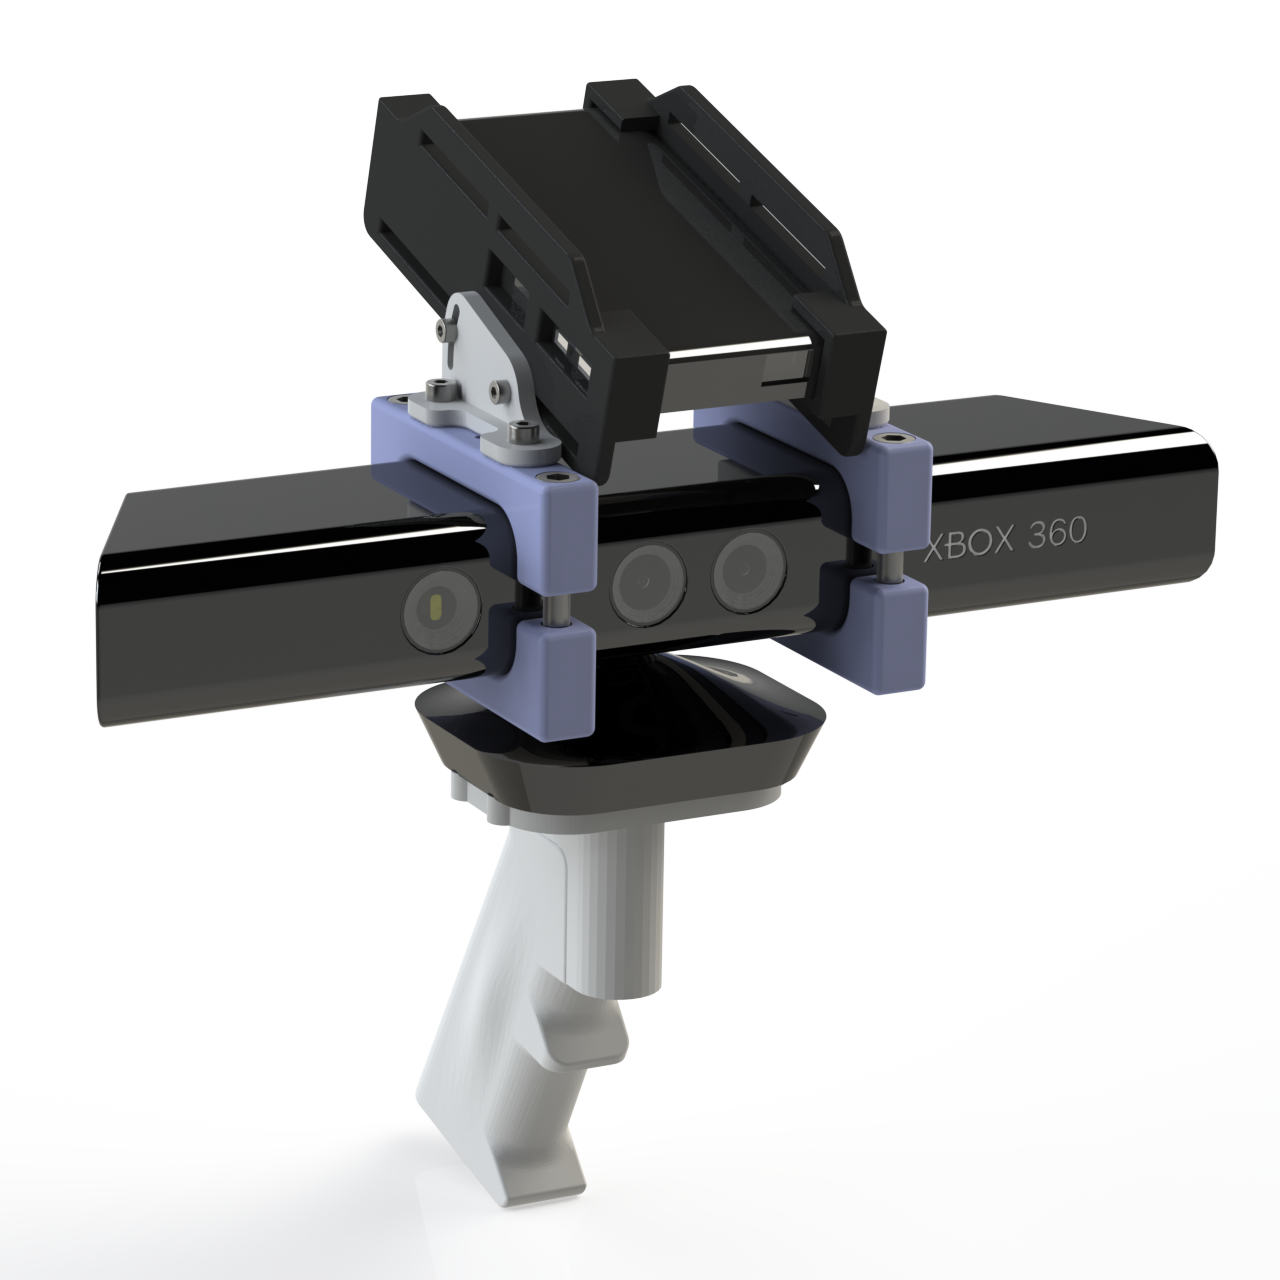
\includegraphics[width = 120mm]{kinpro_KS}
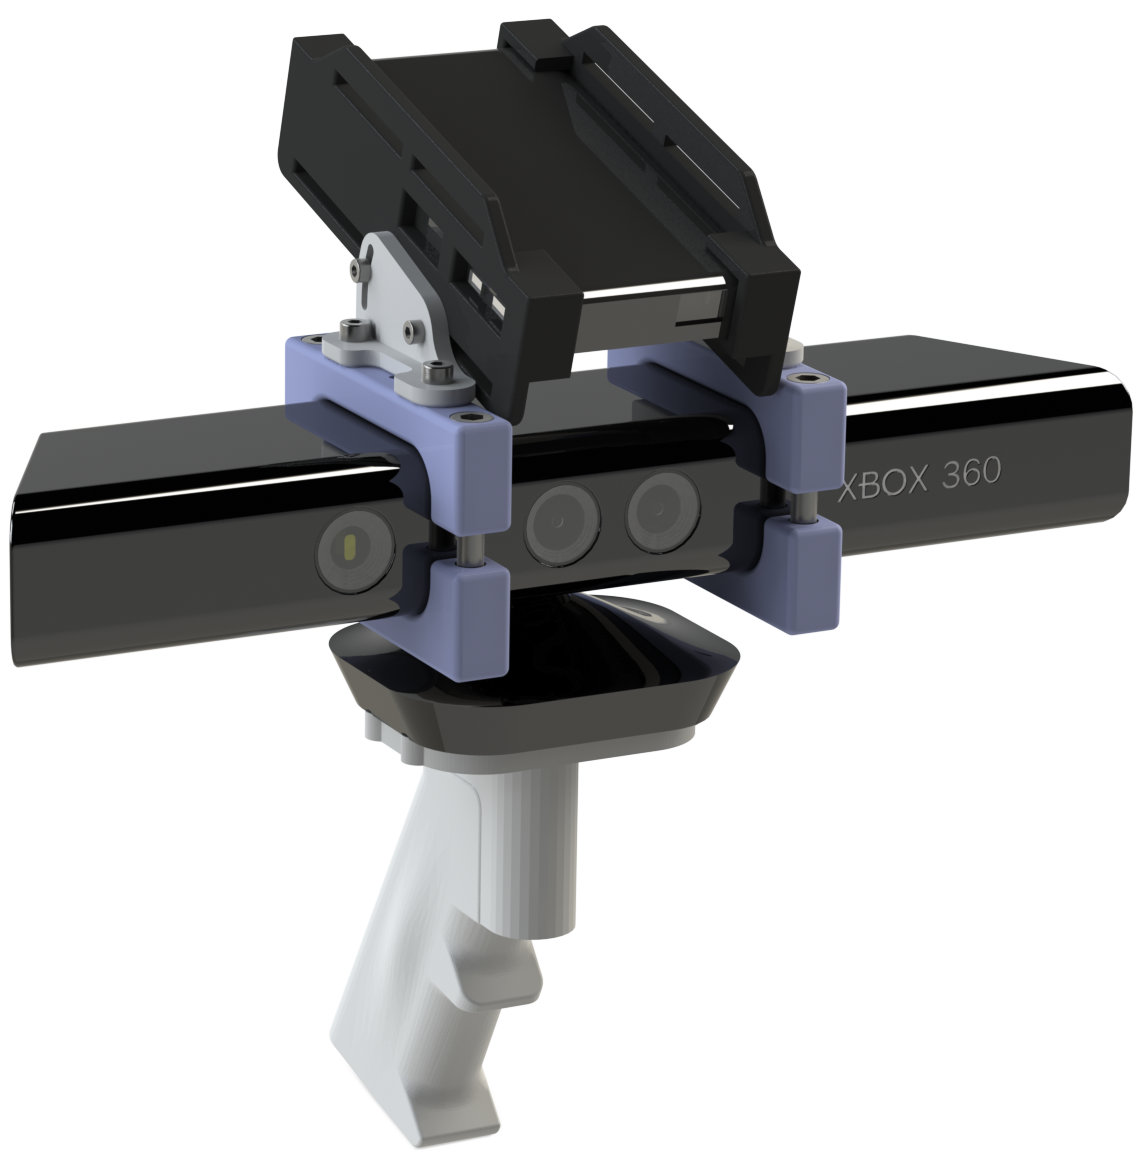
\includegraphics[height = 70mm]{kinpro_KS_cover}

\vfill }
\end{spacing}
\begin{spacing}{1}
\begin{tabular}{l}
 \Large{Diplomarbeit D-03/2014-491}
\end{tabular}

\vspace{5mm}

\begin{tabular}{l}
\large{Lennart Claassen}\\
\large{Matrikelnummer 2576720}
\end{tabular}

\vspace{5mm}

\begin{tabular}{l}
\large{Hannover, März 2015}
\end{tabular}


\vspace{5mm}
{\large
\begin{tabular}{l l}
Erstprüfer  & Prof. Dr.-Ing. T. Ortmaier\\
Zweitprüfer & Prof. Dr.-Ing. J. Wallaschek\\
Betreuer    & M. Sc. Dipl.-Ing. (FH) J.-P. Kobler\\
\end{tabular}
}

\end{spacing}
\end{titlepage}


% --------------------------------------------------
% hier folgt die aufgabenstellung


%\includepdf{pdfs/empty}
%\includepdf{pdfs/AufgabenstellungTeil1}
%\includepdf{pdfs/AufgabenstellungTeil2}

% --------------------------------------------------
% Erkl�rung

\noindent Ich versichere, dass ich diese Diplomarbeit selbstständig
verfasst und keine anderen als die angegebenen Hilfsmittel verwendet
habe.

\vspace{25mm}

\noindent Hannover, 03. März 2015
\newpage

    \clearpage
    \pdfbookmark[0]{\contentsname}{toc}
    %\setcounter{page}{1}
    \tableofcontents                        % Inhaltsverzeichnis
    \listoffigures
    \listoftables
    \printnomenclature                      % Formelverzeichnis einbinden
    \mainmatter                             % der eigentliche Text
		%\input{abkuerzungen}                    % Abk�rzungen im Text, z.B. CI = Cochleaimplantat
		%\input{variablen}                       % Mathematische Variablen
    \chapter{Einleitung und Motivation}

\prever{
%\red[TODO:\\
%%Struktur überarbeiten\\
%%Ausformulieren\\
%virtuelle Daten umformulieren\\
%Quellen für:\\
%- Anwendungsbereiche Visualisierungsverfahren\\
%- Projektions und Bildschirmtechnologien\\
%- Veröffentlichung Kobler\\
%- PA David\\
%- virtuelle Planungsprozesse im Bauwesen\\
%Limitierungen der Systeme -> Wertungsfrei, lediglich nennen (externe Lokalisation etc.)\\
%Modelldaten erläutern\\
%wird in Kapiteleinführung wiederholt sich zu oft\\
%]
%Struktur:\\
%Was ist das Problem, das gelöst werden soll?\\
%Visualisierung in bekannten Umgebungen, AR, Planungsphase von Gebäuden
%Was gibt es für ähnliche Ansätze? Wo kommt der Lösungsansatz her?\\
%Am imes entwickelte Projektor und Lokalisaitonssysteme
%Wie sieht die Lösung aus? Also was wird gemacht?\\
%Daten werden visualisert und modifiziert
%Wie funktioniert die Lösung? Wie wird sie umgesetzt?\\
%kamera-projektoir system zur lokalisatoin und visualisierung und interaktion
%In welcher Weise wird das Problem gelöst?\\
%interaktion merherer beobachter durch projektion möglich, darstellung virtueller Planungsdaten
%Wie ist der Aufbau der Arbeit?\\
%stand der technik, 
%Komponenten, KPS, Software
%lokalisation
%visualisierung
%interaktion
%auswertung
%asublick
}

Die Visualisierung von Informationen nimmt seit jeher einen großen Stellenwert in der menschlichen Kommunikation und Interaktion ein. Die Vermittlung komplexer Sachverhalte lässt sich häufig unter Zuhilfenahme bildlicher Darstellungen vereinfachen. Durch Fortschritte in der Computergrafik konnte die Visualisierung virtueller Modelle in den Alltag integriert werden. Neue technologische Entwicklungen ermöglichen die Erstellung virtueller Welten und erweitern reale Wahrnehmungen durch computergenerierte Bilddaten. Die Anwendungsbereiche komplexer Visualisierungsverfahren reichen von industriellen Planungsvorgängen bei der Umgestaltung von Fertigungssystemen \cite{Lindskog2013} bis hin zur Unterstützung von Chirurgen bei medizinischen Eingriffen \cite{Kersten2013}. Mittels neuer Projektions- und Bildschirmtechnologien werden die möglichen Einsatzgebiete dabei stetig erweitert \cite{Carmigniani2011}.\\

Am Institut für Mechatronische Systeme der Leibniz Universität Hannover wurde ein handgeführtes Projektionssystem aufgebaut, welches die Visualisierung von Zusatzinformationen in der Chirurgie ermöglicht \cite{Kobler2010}. Die Lokalisation des Systems wird dabei über ein externes optisches Navigationssystem realisiert. In einer weiteren Arbeit wurde ein Verfahren entwickelt, um dreidimensionale Oberflächen mittels einer 3D-Kamera zu vermessen und mit hinterlegten Daten von realen Objekten abzugleichen \cite{Reese2013}. Die Repräsentation der Objekte in Form von dreidimensionalen, virtuellen Modellen (Modelldaten) ermöglicht die Registrierung der Oberflächen und die Bestimmung der Position und Orientierung der Kamera bezüglich der realen Objekte. Aufbauend auf diesen Forschungsarbeiten beschäftigt sich die vorliegende Arbeit mit dem Aufbau eines handführbaren \kps{s}, welches die Darstellung visueller Zusatzinformationen in der realen Umgebung ermöglicht. Durch den Abgleich von Sensordaten mit einem virtuellen Modell der Umgebung wird eine Selbstlokalisation des Systems realisiert. Darauf aufbauend können Zusatzinformationen basierend auf Modelldaten lagerichtig in der Umgebung abgebildet und dem Anwender visualisiert werden. Die Interaktion des Benutzers mit den projizierten Daten erlaubt darüber hinaus eine Modifikation der virtuellen Datengrundlage.\\

Das entwickelte Konzept orientiert sich an einem realistischen Anwendungsfall. Im Bauwesen werden Visualisierungen in den virtuellen Planungsprozessen von Neu- und Umbauten genauso wie bei Sanierungen und Innenausbauten eingesetzt \cite{Bouchlaghem2005}. In allen Bereichen kommt es dabei zur regelmäßigen Kommunikation zwischen den am Prozess beteiligten Personen, zu denen unter anderem Architekten, Bauingenieure, Techniker und Bauherren zählen. Konzeptions- und Bewertungstreffen innerhalb der Gebäude sind daher fester Bestandteil der Planungs- und Ausführungsvorgänge. Das aufgebaute \kps{} erlaubt es, virtuelle Planungsdaten in diesen Umgebungen zu visualisieren. Durch die Interaktion der Beobachter mit der Projektion werden Modifikationen der Modellumgebung ermöglicht, welche direkt in den virtuellen Planungsprozess zurückgeführt werden können. Die Methode der Projektion ist dabei besonders als Basis der Kommunikation und Kooperation geeignet, da die Visualisierungen allen beteiligten Personen zur gleichen Zeit zugänglich sind.\\

Zu Beginn dieser Arbeit wird in \kapitel{chap.tech} ein Überblick über den aktuellen Stand der Technik im Bereich der Lokalisation mobiler Systeme, insbesondere handgeführter Projektionssysteme gegeben. In \kapitel{chap.material} erfolgt eine Beschreibung des aufgebauten \kps{s} und seiner Komponenten. Des Weiteren erläutert das Kapitel die Kalibrierung der 3D-Kamera und des Projektors, mittels welcher die Abbildungstransformationen bezüglich der Umgebung bestimmt werden. Anschließend folgt die Vorstellung der verwendeten Softwarebibliotheken und der entwickelten Programmstruktur. Die Datengrundlage für die Modellumgebung und die virtuellen Modellobjekte ist in \kapitel{chap.modeldata} spezifiziert. \kapitel{chap.loc} beschreibt die eingesetzten Lokalisationsverfahren zur Bestimmung und Verfolgung der Position und Orientierung des \kps{s} innerhalb der Umgebung. Der in \kapitel{chap.vis} beschriebene Visualisierungsvorgang umfasst die perspektivisch korrekte Projektion virtueller Objekte und die Ergänzung der Visualisierung um zusätzliche Informationen. \kapitel{chap.interaction} erläutert den implementierten Interaktionsansatz, welcher Benutzereingaben durch Auswertung von Tiefeninformationen der 3D-Kamera detektiert. Experimentelle Untersuchungen zur Bewertung der Robustheit und Performanz des Systems werden in \kapitel{chap.results} vorgestellt. Dabei wird neben der Genauigkeit der Lokalisation und Projektion auch die Latenzzeit der Visualisierung analysiert und bewertet. Abschließend fasst \kapitel{chap.zusammenfassung} die durchgeführten Arbeiten zusammen und gibt eine Ausblick auf mögliche Erweiterungen und Optimierungen des aufgebauten \kps{s}.

%Bauwesen als Oberbegriff
%Innenarchitekt(ur), Architekt, Bauingenieur, Bauherr
%Innenausbau, Sanierung, Modernisierung, Umbau
%
%Ziel der Arbeit/Motivation:\\
%Bei der Planung von Gebäuden oder anderen Bauten kann es erforderlich sein die Planungen von bestimmten Strukturen nach Erstellung des Rohbaus innerhalb des realen Modells zu überprüfen. Dies ermöglicht die Erkennung von Planungsfehlern sowie die Änderungen der Planungsdaten und kann somit Verzögerungen während der Bauphase entgegenwirken.\\
%
%Lokalisation in aus Modelldaten bekannter Umgebung.\\
%Um die Planungsdaten überprüfen zu können ist es erforderlich, dass die Position des entwickelten Systems innerhalb der realen Umgebung erkannt wird um einen Abgleich mit den Planungsdaten zu ermöglichen.\\
%Die Modelldaten liegen dabei vor, z.B. als 3D-Modell eines Gebäudes oder Raumes. Ziel ist daher zunächst die Ermittlung der aktuellen Pose des Systems innerhalb der Umgebung. Um die räumliche Lokalisation zu ermöglichen verfügt das System über eine RGB-D Kamera (Microsoft Kinect) welche ein Abbild der Umgebung in Form einer Punktewolke erstellt. Die dadurch ermittelten Tiefendaten können dann dazu verwendet werden einen Abgleich zwischen Modell und Realität durchzuführen. Um die Genauigkeit zu erhöhen und den Rechenaufwand der Lokalisation zu verringern verfügt das System darüber hinaus über eine Inertialmesseinheit (IMU) mit welcher die Orientierung im Raum bezüglich der Drehachsen \glqq Roll\grqq\space und \glqq Pitch\grqq\space bestimmt werden kann.\\
%Sobald die initiale Position des Systems im Raum detektiert wurde, erfolgt ein Tracking der Systemposition durch Fusionierung von visuellen Odometriedaten mit Lage- und Beschleunigungsdaten, welche durch die IMU ermittelt wurden.\\
%
%Projektion von Modellstrukturen.\\
%Nachdem die Position des Systems innerhalb der Umgebung bestimmt wurde, sollen bestimmte Strukturen und Informationen visualisiert werden. Dazu verfügt das entwickelte System über einen Laser-Projektor, mit welchem die gewünschten Visualisierungen auf Wände und Objekte projiziert werden können. Es ist dazu erforderlich die Position bzw. die Perspektive des Projektors innerhalb der Umgebung zu bestimmen. Hierzu wird im Vorfeld eine Kalibrierung des Kamera-Projektor-Systems durchgeführt, sodass die Projektorperspektive durch eine Koordinatentransformation bestimmt werden kann.\\
%
%Detektion von Benutzereingaben.\\
%Die projizierten Informationen sollen dazu dienen, eine Überprüfung und Bewertung der Planungsdaten durch den Benutzer vornehmen zu können. Um eine direkte Korrektur oder Modifikation der Daten zu ermöglichen ist es daher erforderlich, dass der Benutzer mit dem System bzw. der Visualisierung interagieren kann. Das System muss daher in der Lage sein, Benutzereingaben zu erkennen und zu verarbeiten. Dazu wird ebenfalls die Kinect verwendet, um durch Auswertung des Tiefenbildes die Benutzeraktionen zu erkennen.\\
%
%Modifikation des Modells.\\
%Sobald eine Benutzereingabe erkannt wurde, wird diese ausgewertet und entsprechend verarbeitet. Je nach Auswahl können somit die Modellelemente modifiziert werden.\\

\prever{
%\red[Allgemeine Einführung zu Piko Projektoren und welche Möglichkeiten sie bieten.]\\%
%Projektion ermöglicht die Kooperation zwischen Personen, da sie von allen Parteien zu sehen ist!
}										% die einzelnen Kapitel einbinden
	\chapter{Stand der Technik}
\label{chap:tech}
%\red[TODO:\\
%Lokalisation mobiler Systeme in Gebäuden etc.\\
%Augmented Reality inkl. Interaktion mit Projektionen\\
%Handgeführte Lokalisationssysteme (Ohne Projektion)\\
%]
\red[Viele Forschungsgruppen beschäftigen sich mit der Problematik, sowohl Lokalisation in bekannter als auch unbekannter Umgebung.
Da das Ziel des entwickelten Systems in der Lokalisation in bekannter Umgebung liegt wird sich bei der Darstellung der bisherigen Forschungsansätze auf diesen Bereich konzentriert. Da das entwickelte System aufgrund seiner Komponenten dafür ausgelegt ist, die Lokalisation auf Basis von Tiefen- und Farbinformationen durchzuführen werden an dieser Stelle Ansätze, welche auf anderen Verfahren wie Ortung von Funkwellen basieren, ebenfalls nicht näher ausgeführt.]\\


Da sich die geplante Anwendung des \kps{s} in verschiedene Funktionsbereiche gliedern lässt, soll im Folgenden ein Überblick über den aktuellen Forschungsstand innerhalb der jeweiligen Bereiche gegeben werden. Abschließend werden Systeme vorgestellt, welche eine mit dem in dieser Arbeit entwickelten \kps{} vergleichbare Funktionalität in einem oder mehreren Bereichen bieten.

\section{Lokalisation}
\label{chap:mcl}
\red[Die Lokalisation mobiler Systeme in bekannten Umgebungen ist Gegenstand aktueller Forschungsvorhaben.]\\
Aufgrund des Anwendungsgebietes des entwickelten \kps{s} beschränkt sich der folgende Überblick auf die Lokalisation von mobilen Systemen in Innenräumen. Aus diesem Grund werden ebenfalls keine Lokalisationsverfahren betrachtet, die auf der Verwendung von externer Sensorik zur Bestimmung der Systempose basieren.\\
Die Selbstlokalisation mobiler Systeme hat sich besonders in der Robotik in den letzten Jahrzehnten zu einem wichtigen Forschungsbereich entwickelt, da sie eine Voraussetzung für die autonome Navigation von Robotersystemen darstellt \red[Andere Forschungsbereiche?].\\
Zu unterscheiden ist dabei zwischen den Verfahren der globalen und lokalen Lokalisation. Bei der globalen Lokalisation soll die absolute Pose\footnote{Die Pose eine Systems umfasst die Beschreibung seiner Position und Orientierung bezogen auf die sechs räumlichen Freiheitsgrade \red[Formel oder Quelle?]} des Systems innerhalb seiner Umgebung ermittelt werden. Die lokale Lokalisation bezieht sich hingegen auf die Bestimmung einer relativen Transformation zwischen dem vorhergehenden und dem aktuellen Zustand. Während die globale Lokalisation damit meist angewendet wird um die initiale Pose in einer bekannten Umgebung festzulegen dient die lokale Lokalisation dazu die Veränderungen der Systempose kontinuierlich zu verfolgen.\\ \red[Begriff Tracking nennen?\\]
Eine weitere Unterscheidung innerhalb dieser Ansätze wird dabei nach der Anzahl der betrachteten Hypothesen vorgenommen. Während unimodale Lokalisationsverfahren sich auf eine Hypothese zur Bestimmung der Systempose beschränken, werden bei multimodalen Lokalisationsverfahren mehrere Hypothesen parallel betrachtet.
%Im Folgenden soll ein Überblick über verbreitete Lokalisationsansätze gegeben werden.
%Unimodale Ansätze berücksichtigen jeweils nur eine Pose, während bei multimodalen Verfahren mehrere Posen gleichzeitig aufrechterhalten werden.
\subsection{Unimodale Lokalisationsverfahren}
Da bei unimodalen Verfahren nur eine mögliche Pose des Systems betrachtet wird, erfordert der Einsatz im Rahmen einer globalen Lokalisation damit meist die \red[(sinnvolle)] Hypothese eines Anfangszustands. Vornehmliche Anwendung finden sie daher im Bereich der lokalen Lokalisation. \red[Darauf eingehen, welche Verfahren im Rahmen dieser Arbeit interessant sind/warum einige nicht behandelt werden sollen]

Einen vergleichsweise einfachen Ansatz stellt das sogenannte Scan Matching \red[Wie kenntlich machen? Quotes oder kursiv? Fett?] dar. Dieses Verfahren bezeichnet den Abgleich \red[(Matching)] von Messungen der Umgebungen mit vorangegangenen Messungen \cite{Gutmann1996} oder zuvor aufgezeichneten Vergleichsdaten \cite{Gutmann1998}. Durch Bestimmung der maximalen Überlappung kann die translatorische und rotatorische Veränderung der Pose bezüglich der Referenz berechnet werden. Die betrachteten Messwerte sind dabei meist Distanzen, welche beispielsweise mit Laser- \cite{Diosi2007} oder Ultraschall-Entfernungsmessern \cite{Burguera2005} aufgezeichnet wurden. Die Berechnung der Transformationsvorschrift zwischen den Zuständen erfolgt auf Basis verschiedener Algorithmen wie dem \textit{Iterative Closest Point} Verfahren (ICP) \cite{Besl1992}\cite{Lu1994} oder der \textit{Normal Distributions Transformation} (NDT) \cite{Biber2003}.\\

Das \red[Line Matching] erweitert diesen Ansatz, indem es die häufig geradlinige Struktur von Innenräumen nutzt. Anstelle einzelner Messpunkte werden Linien aufeinander abgeglichen, wodurch die Robustheit der Lokalisation gesteigert werden kann. Die Linien werden dabei aus den Messwerten extrahiert und mit zuvor erstellten Liniendaten aus Umgebungskarten verglichen \cite{Cox1991}\cite{Gutmann1999}. Auch ein umgekehrtes Vorgehen ist möglich, in welchem die Liniendaten der Karten in äquidistante Punktmengen transformiert und mit den Daten der Entfernungsmessung abgeglichen werden. In diesem Fall reduziert sich die Berechnung der Überdeckung auf ein abgleichen von Punkten, welches mit den Algorithmen des Scan Matching gelöst werden kann.\\
Eine Erhöhung der Komplexität wird durch die Betrachtung von Polylinien, also zusammenhängenden Linienelementen erreicht \cite{Wolter2004}. Zur Lösung können dabei Algorithmen angewendet werden, welche für das Abgleichen von Formen entwickelt wurden und ursprünglich aus der computergestützen Bildverarbeitung stammen.\\
Eine andere Art von Ansätzen des Line Matchings verfolgt die Beschreibung der Liniendaten mittels verschiedener Deskriptoren wie Länge, Abstand und Winkel \cite{Frey2014} \cite{Garulli2005}. Dieses Vorgehen ermöglicht eine kompaktere Darstellung der relevanten Umgebungsmerkmale und bildet den Übergang zu den merkmalsbasierten Lokalisationsverfahren.\\

Merkmalsbasierte Lokalisation beschreibt eine allgemeinere Anwendung des Prinzips von Deskriptoren (Features) zur Ermittlung der aktuellen Pose eines Systems. Betrachtet werden je nach Anwendungsfall und verwendeter Sensorik unterschiedlichste Merkmale. Neben Distanzmessungen \cite{Tomono2004} werden insbesondere auch Kamerasysteme verwendet um Merkmale aus der Umgebung zu extrahieren \cite{Se2001}. Durch die hier ebenfalls vorhandene Nähe zu Anwendungsfällen in der computergestützten Bildverarbeitung kann auf eine Vielzahl von Algorithmen aus diesem Forschungsbereich zurückgegriffen werden. Da die Definition geeigneter Deskriptoren darüber hinaus bei der Verwendung von Entfernungsmessern häufig nicht generalisierbar ist \red[belegen!?], hat sich für die merkmalsbasierte Lokalisation die Verwendung von Bilddaten als Basis bewährt und wird unter dem Begriff der visuellen Odometrie \cite{Mccarthy2003} zusammengefasst.\\
%Definition der Deskriptoren bei Laserscan etc. schwierig und Anwendungsabhängig -> hauptsächlicher Einsatz von merkmalsbasierter Lokalisation bei visuellen Daten (Kamerabildern) \red[visuelle Odometrie fällt darunter!] SIFT/SURF, PCA.

Ein weiteres unimodales Lokalisationsverfahren ist die Schätzung und Verfolgung der Systempose mittels eines Kalman-Filters\red[Fußnote oder Verweis auf Beschreibung später?; Monomodale Variante des Bayes Filters]. Dieses Verfahren kann auf den bisher beschriebenen Matching Verfahren aufbauen, ist dabei jedoch nicht auf diese limitiert. Durch das Kalman-Filter wird eine Fusionierung der Sensordaten mit der Odometrie \red[schon beschrieben?] erreicht, wobei die Sensordaten beispielsweise aus globalen Kartenmerkmalen ermittelt werden \cite{Leonard1991} oder aus der Kombination verschiedener Sensoren \cite{Roumeliotis1997} resultieren. Ein großer Vorteil dieses Lokalisationsverfahrens liegt somit darin, mehrere Datenquellen in einem Modell vereinen zu können.\\ Da das Kalman-Filter die Pose mittels einer Wahrscheinlichkeitsdichtefunktion annähert eignet er sich besonders unter der Voraussetzung, dass eine Approximation der initialen Pose vorliegt. Als globales Lokalisationsverfahren bei unbekannter Startpose eignet sich der Kalman-Filter dagegen nur bedingt. Diese Limitierung kann jedoch durch parallele Verwendung multipler Kalman-Filter, also dem Einsatz eines multimodalen Lokalisationsverfahren, überwunden werden.
%Anwendung des Kalman-Filters auf mehrere Hypothesen führt zu multimodalen Lokalisationsverfahren. 
%EKF approximiert Verteilung lokal als Gaußverteilung
\subsection{Multimodale Lokalisationsverfahren}
Multimodale Lokalisationsverfahren erhalten stets mehrere Hypothesen möglicher Systemposen aufrecht. Dadurch ermöglichen sie neben einer globalen Lokalisation ohne Anfangshypothese auch das Wiedererlangen richtiger Posen nach fälschlicher Lokalisation in lokalen Minima. Im Falle einer fehlerhaften Lokalisation ist beispielsweise das Scan Matching zwar in der Lage die Überdeckung zwischen Sensordaten und lokaler Kartenumgebung zu minimieren, der Algorithmus erkennt jedoch nicht, ob sich das System global betrachtet an einer falschen Stelle befindet. Wichtig wird dieser Aspekt insbesondere beim sogenannten \textit{kidnapped robot scenario}, bei welchem das System im Betrieb aus seiner bekannten Pose in eine unbekannten Pose gebracht wird \cite{Yic2011} ohne dabei Sensordaten zu verwerten. Multimodale Verfahren können dem begegnen, indem sie stets eine Anzahl \textit{n} an Posen mit der höchsten Plausibilität betrachten und in jedem Lokalisationsschritt zufällige Posen in die Betrachtung integrieren.\\

Das bei der Markov Lokalisation angewendete Prinzip basiert auf einer Diskretisierung des Posenraums. Für jeden Freiheitsgrad des Systems wird eine Rasterkarte erstellt, in welcher die Gitterzellen mögliche Posen innerhalb des diskreten Raumes repräsentieren. Jede Hypothese wird über eine Wahrscheinlichkeitsdichte abgebildet, welche auf Basis von Varianten des Bayes Filter \red[erklären? wo?] bestimmt wird, zu denen auch das Kalman Filter gehört \cite{Hertzberg2012}. In jedem Lokalisationsschritt werden Odometrie- \red[schon erklärt?] und Sensordaten verarbeitet und die Wahrscheinlichkeitsdichte der Gitterzellen basierend darauf angepasst. Da selbst bei deutlichem Anstieg der Probabilität einer Pose auch die weiteren diskreten Posen in der Betrachtung erhalten bleiben, ist das System stets in der Lage auf falsche Lokalisationen zu reagieren.\\
Die globale Lokalisation erfolgt bei der Markov Lokalisation entweder durch Initialisierung mit einer Gleichverteilung über alle Zellen, oder durch eine Initialisierung mit Normalverteilung und geringer Varianz um die Hypothesen der Startpositionen \cite{Hertzberg2012}.\\

Die Diskretisierung und gleichzeitige Betrachtung aller möglichen Posen ist mit großem Rechenaufwand verbunden. Die Monte Carlo Lokalisation ist in der Lage dieses Problem zu umgehen, indem es anstelle aller möglichen Posen nur ausgewählte Stichproben betrachtet. Jede dieser Stichproben entspricht einer Pose und wird auch als Partikel bezeichnet. Die Partikel können dabei neben dem diskreten Posenraum auch aus dem kontinuierlichen Posenraum, wie er meist für mobile Systeme vorliegt, gezogen werden \cite{Fox2001}. Die Kontrolle über die Partikelanzahl ermöglicht es zudem, den Algorithmus auf die verfügbaren Rechenressourcen abzustimmen \cite{Thrun2001}.\\
Durch die geringen Einschränkungen bezüglich der als Basis verwendeten Wahrscheinlichkeitsverteilungen ist die Monte Carlo Lokalisation in der Lage die globale und lokale Lokalisation mit hoher Genauigkeit zu realisieren \cite{Thrun2005}. Die hohe Effizienz dieses Ansatzes führt dazu, dass er bei der Lokalisation mobiler Systeme der Markov Lokalisation deutlich überlegen ist \cite{Fox2001}.

%\red[Monte Carlo etc. ->Buch\\]
%\red[smartphone lokalisierung thematisieren aber verwendet externe Sensorik zur Positionsbestimmung]

\red[In der Robotik wird die fortlaufende Ableitung der Orientierung und Geschwindigkeit aus Messungen der Raddrehwinkel als Odometrie bezeichnet. \cite{Hertzberg2012}\\]
\red[Wie Quelle für Lokalisationsabsatz referenzieren?]
%\red[Welche Lokalisationsverfahren gibt es. Allgemein und speziell für handgeführte Systeme.]\\


\section{RGB-D Kameras/Tiefenkameras(?)}
Die beschriebenen Verfahren und Algorithmen haben sich besonders im Bereich der 2D Lokalisation bewährt, obwohl sie prinzipiell unabhängig von der Anzahl an Dimensionen sind. Die größer werdende Verbreitung von zugleich kostengünstigen und leistungsfähigen Tiefenkameras wie der Microsoft Kinect\red[Tm] führt jedoch dazu, dass die Anwendungen immer häufiger auch auf 3D Umgebungen erweitert werden. Die Lokalisation in 3D Umgebungen ist besonders dann von Bedeutung, wenn das System sich in mehr als einer Ebene bewegen kann. Die Anzahl der Freiheitsgrade (in der 2D Lokalisation meist drei) steigt dadurch auf sechs an, da die Pose des Systems nun über drei translatorische sowie drei rotatorische Freiheitsgerade beschrieben wird. Neben der Notwendigkeit für geeignete 3D Modellumgebungen kann die Erhöhung der Freiheitsgrade auch dazu führen, dass keine Odometriedaten mehr ermittelt werden können. Dies ist insbesondere bei fliegenden \cite{Huang2011} und hand- oder körpergeführten Systemen \cite{Fallon2012} der Fall. Die Auswertung von Tiefen- und Farbinformationen ermöglicht es jedoch dies durch visuelle Odometrie zu kompensieren \cite{Whelan2013robust}.\\
Auch die Integration in traditionelle Robotersysteme zeigt, dass Tiefenkameras eine sinnvolle Alternative zu bisherigen Sensoren wie Laser-Entfernungsmessern darstellen können \cite{Cunha2011} \cite{Eriksson2012}. Anzumerken ist, dass der beobachtbare Bildbereich bezüglich Distanz und Sichtfeld meist deutlich kleiner ist als bei Laser Sensoren. Die Eignung von Tiefenkameras für Lokalisationsaufgaben ist daher anwendungsabhängig zu überprüfen.\\

%\red[Featurebasierte Lokalisation (RGB-D SLAM, Fovis)\\
%Markerbasierte Lokalisation]\\

\section{Augmented Reality}
Die Überlagerung oder Vereinigung von virtuellen und realen Umgebungen wird als Augmented Reality (AR) bezeichnet \cite{Azuma1997}. Durch eine dreidimensionale Registrierung wird die Interaktion zwischen den Objekten der beiden Welten ermöglicht. Die Umgebung des menschlichen Beobachters wird somit um virtuelle Elemente ergänzt. Neben herkömmlichen und transparenten Bildschirmen \red[quellen? google glass!?] werden insbesondere Projektoren zur Visualisierung der virtuellen Daten eingesetzt. Anwendungen finden sich in der Medizin als Unterstützung von Ärzten in der Chirurgie \cite{Gavaghan2012} \cite{Hoppe2001} oder als Hilfe bei der Kommunikation zwischen Arzt und Patient \cite{Bluteau2005}. Durch Zusatzinformationen kann AR die Interaktionsmöglichkeiten mit Robotersystemen erweitern \cite{DeTommaso2012} oder statische Objekte animieren \cite{Raskar1999}. In Alltagssituationen entsteht durch die Visualisierung von Informationen eine interaktive Benutzerschnittstelle \cite{Linder2010} \cite{Huber2012}.\\
Durch Kombination mehrerer Projektoren können virtuelle Umgebungen auf realen Geometrien erzeugt \cite{Low2001} oder der Interaktionsbereich auf weiter entfernte Oberflächen ausgedehnt werden \cite{Wilson2010}.

%\red[Low - Life-Sized Projector Based Dioramas -> Hausumgebung auf leere Wände projiziert]\\
%\red[Oh - Projektion von Entertainment/Filmen etc. auf Oberflächen]\\
%\red[Raskar - Table-Top AR, Bringing Physical Models to life]\\
%\red[Huber - Lightbeam -> Interaktion mit Projektionen über Alltagsgegenstände]\\
%\red[Linder - LuminAR -> Interaktion mit Projektion in Büroumgebung]\\
%\red[Wilson - Interaktion zwischen mehreren Oberflächen durch Einsatz mehrerer Projektoren und Kameras]

\red[Bimber - Embedded Entertainment with Smart Projectors -> für Ausblick/Limitierungen bzgl. der Projektionsuntergründe]
\red[auch Park - Kontrast erhöhung]
\red[auch Wang - Relighting]\\%
\red[Bimber - Multi-Projector Techniques for Real Time... -> Architectural Projection]\\

%\section{Interaktion}
%\red[Benutzerinteraktion basierend auf der Verwendung von Tiefeninformationen. Hauptsächlicher Ansatz ist die Befehlsvorgabe über Gestensteuerung.]\\
%\red[Welche Formen von Benutzerinteraktion gibt es, besonders bezogen auf die Kinect und Projektionssysteme.\\
%(z.B. Omnitouch)]\\

%\red[Wen - Handgesten zur Interaktion in der Chirurgie]\\



\section{Handgeführte Projektionssysteme}
%\subsection{Lokalisation}
%\red[Ein handgeführtes Scanning System, entwickelt von Mair \textit{et al.} \cite{Mair2010}, fusioniert IMU Daten und  \\]

%\subsection{Projektion}
Die Miniaturisierung der Projektionstechnologie hat zu einer Entwicklung mobilerer, handgeführter Systeme geführt. In den letzen Jahren wurden verschiedene Ansätze untersucht, welche sich mit der Projektion virtueller Zusatzinformationen durch tragbare Systeme befassen. Dabei werden sowohl Miniprojektoren als auch in Smartphones integrierte Projektionssysteme eingesetzt. Im folgenden soll ein Überblick über vorhandene handgeführte Projektionssysteme und ihre Anwendungsbereiche gegeben werden.\\
Die Navigation innerhalb eines Museums wird von Wecker \textit{et al.} \cite{Wecker2013} mittels handgeführter Projektionssysteme durch die Visualisierung von Karten- und Wegdaten unterstützt.\\
Ein System mit ähnlichem Ziel haben Chung \textit{et al.} \cite{Chung2011} entwickelt. Dieses soll dem Anwender bei der Navigation innerhalb von Gebäuden behilflich sein. Ein Miniprojektor wird dabei in Kombination mit einem Smartphone verwendet um zusätzliche Informationen bei der Erkennung von Visitenkarten oder Gebäudeplänen zu visualisieren. Die Funktionalität soll dabei an eine Taschenlampe erinnern, welche die Zusatzinformationen sichtbar macht.\\
Auch Li \textit{et al.} \cite{Li2013} stellen ein handgeführtes Projektionssystem vor, welches im Konzept an eine Taschenlampe angelehnt ist. Durch Projektion von Karten- und Wegdaten auf den Boden vor dem Benutzer wird dieser entlang eines Weges geführt. Im Gegensatz zu Chung \textit{et al.} erfolgt dabei eine kontinuierliche Aktualisierung der Projektion in Abhängigkeit der Position entlang des Weges. Die Lokalisation wurde dabei manuell durch eine Begleitperson vorgenommen.\\
Molyneaux \textit{et al.} \cite{Molyneaux2012} erweitern die Metapher der Taschenlampe und integrieren darüber hinaus eine automatische Lokalisation des handgeführten Projektionssystems. Eine Infrastruktur aus Microsoft Kinect Sensoren erkennt und verfolgt die Systempose und ermöglicht dadurch die verzerrungsfreie Projektion beliebiger Zusatzinformationen innerhalb eines Raumes. Durch Infrarot Kameras am Projektionssystem selbst wird zudem eine Interaktion mit den visualisierten Daten realisiert.\\
Das \textit{SideBySide} Projekt von Willis \textit{et al.} \cite{Willis2011} ermöglicht die Interaktion zwischen Benutzern über handgeführte Projektionssysteme. Jedes System projiziert dabei sowohl ein Bild im sichtbaren Lichtspektrum als auch einen Marker im Infrarot Spektrum. Die Erkennung der Marker durch die Systeme erlaubt das Zusammenspiel der jeweiligen Projektionen der Anwender. Beispielanwendungen finden sich im Austausch von Informationen oder Dateien und in kooperativen Spielen.\\
Einen weiteren Ansatz für kooperative Projektionssysteme liefern Robinson \textit{et al.} \cite{Robinson2012} mit \textit{PicoTales}. Dabei werden handgeführte Projektionssysteme verwendet um gemeinsam animierte Videos zu erstellen. Die Lokalisation erfolgt dabei nach einem Kalibrierungsverfahren über das Aufzeichnen von Bewegungsdaten durch eine inertiale Messeinheit. Die Auswertung und Fusionierung zu einem gemeinsamen Video erfolgt nach Ende der Interaktion über einen separaten Computer.\\
Das von Harrison \textit{et al.\ }\cite{Harrison2011} entwickelte \textit{Omnitouch} ist ein körpergeführtes System, welches die Projektion grafischer Benutzeroberflächen auf typische im Alltag vorhandene Oberflächen ermöglicht. Das System verfügt neben einem Projektor auch über eine Tiefenkamera zur Detektion von Benutzereingaben. Dadurch wird die Funktionalität von Touchscreens abgebildet und es können typische Anwendungen implementiert werden, die sonst beispielsweise auf Smartphones oder Tablets genutzt werden.\\
Ein vergleichbarer Aufbau wird von Tan \textit{et al.} \cite{Tan2013} verwendet um virtuelle Modelldaten auf reale Modelle zu projizieren. Dies ermöglicht die korrekte Darstellung der virtuellen Daten auch bei einem Wechsel der Beobachterperspektive. Die Lokalisation des Systems erfolgt dabei anhand des Abgleichs zwischen Modell und Sensordaten.\\

\red[Abbildungen der Systeme?\\]

%Warum der Ansatz?
Wenige der handgeführten Systeme ermitteln ihre Pose innerhalb der Umgebung. Häufig ist lediglich die relative Pose bezüglich definierter Oberflächen oder Objekte Bestandteil der Betrachtung. Systeme, welche eine globale Lokalisation erfordern, verwenden dagegen entweder manuelle oder auf externen Sensoren basierende Lokalisationsverfahren. Die Selbstlokalisation mobiler Systeme ist allerdings seit einiger Zeit Forschungsthema und es existiert eine Vielzahl von Ansätzen um eine zuverlässige Lokalisation in zwei- und dreidimensionalen bekannten Umgebungen zu erreichen. Eine Übertragung auf den Anwendungsbereich handgeführter Projektionssysteme hat jedoch bisher nicht stattgefunden.\\
Die vorliegende Arbeit soll die Lücke zwischen der Lokalisation mobiler Systeme und der projektorbasierten \textit{Augmented Reality} schließen. Die Anwendungsgebiete werden vereint, indem die Selbstlokalisation eines handgeführten \kps{s} realisiert und darauf aufbauend die Projektion visueller Zusatzinformationen in der realen Umgebung ermöglicht wird.
\red[Zwei Lokalisationsansätze verwendet, globale Lokalisation und visuelle Odometrie]
%\red[Verschiedene handgeführte Systeme, welche jedoch entweder auf manueller, externer Lokalisation, oder markerbasierter Lokalisation beruhen. Bei anderen Systemen wird lediglich eine Ausrichtung bzgl der Projektionsoberfläche durchgeführt. Selbstlokalisation ohne Hilfsmittel (externe Sensorik, Marker in Form von KArten o.ä.) bisher nicht behandelt. Lokalisation von mobilen Systemen allerdings seit einiger Zeit Forschungsthema, neuer ist jedoch die 3D Lokalisation. System soll die Brücke bilden zwischen mobilen, autonomen Lokalisationssystemen und handgeführten Projektionssystemen\\]
\red[OHNE HILFSMITTEL nochmal aufgreifen wenn alternative Lokalisation über Muster o.ä. aufgeführt wird]

\red[Tan - iSarProjection -> Handgeführtes System, Aufbau sehr ähnlich Kinpro, Lokalisation aber anhand der Modelle auf die dann projiziert wird, eher wie David]\\

\red[Welche Systeme gibt es zur Projektion von (Modell-)Daten.]\\

%\includesvgnew[1]{test}

	\chapter{Material}
\label{chap:material}

\section{Hardware}
Das erstellte System wurde aus verschiedenen Hardwarekomponenten aufgebaut, welche im Folgenden näher beschrieben werden sollen.

\subsection{Microsoft Kinect}

\subsection{Microvision Pico Laser Projektor}

\subsection{Arduino Nano}

\subsection{Inertialmesseinheit}

\subsection{Raspberry Pi}

\section{Software}
Zur Realisierung der einzelnen Systemfunktionen wurden Softwarekomponenten erstellt welche auf verschiedenen Softwarebibliotheken aufgebaut sind. Die Bedienfunktionen des Systems wurden dabei innerhalb einer grafischen Benutzeroberfläche zusammengefasst.

\subsection{Open Source Computer Vision Library}
\cite{OpenCV}.

\subsection{Qt}
Die von der Firma Trolltech entwickelte und mittlerweile von der Firma Digia verwaltete Qt Bibliothek ermöglicht eine plattformunabhängige Entwicklung von grafischen Benutzerschnittstellen im C++ Standard \cite{Qt}.

\subsection{ROS}

\subsection{PCL}

\subsection{VTK}

\subsection{GUI}
Mit aufnehmen in dieser Liste?


	\chapter{Datengrundlage}
\label{chap.modeldata}
\red[TODO:\\
Verschiedenen Dateitypen nennen?\\
Verwendete Programme nennen? Binvox, blender etc.?\\
Dateistruktur -> Sichern von Daten/Rückkopplung des veränderten Modells hier einfügen?\\
]

Das Ziel der Anwendung liegt in der Darstellung von Modelldaten durch das \kps{} innerhalb der realen Umgebung. Dazu wird in diesem Kapitel eine geeignete Datenstruktur definiert. Als Grundlage für die spätere Lokalisation ist es erforderlich, ein möglichst originalgetreues Abbild der realen Umgebung zu erstellen. Diese Modellumgebung ermöglicht bei hoher Modellgüte die präzise Positionierung virtueller Objekte in der realen Umgebung.\\

Die zu visualisierenden Modellobjekte werden anhand der virtuellen Umgebungsdaten orientiert und positioniert und können über einen Abgleich in die reale Umgebung übertragen werden. Die Projektion der Modellumgebung selbst innerhalb der realen Umgebung würde lediglich zu Überlagerungen gleicher Strukturen führen und besitzt außerhalb von Validierungen des \kps{s} keine Relevanz.\\

\section{Modellumgebung}
\label{chap.slam}
Für die Verwendung der erstellten Programmstruktur ist es erforderlich, dass die Umgebung in Form eines 3D-Modells abgebildet wird. Als Modellumgebung werden dabei alle statischen Objekte und Strukturen betrachtet, welche eine Repräsentation der realen Umgebung darstellen. Um die benötigten Daten zu generieren können verschiedene Verfahren angewendet werden.\\
Liegen bereits Modelldaten der Umgebung vor, so kann das virtuelle Umgebungsmodell direkt aus diesen abgeleitet werden. Insbesondere ist dies der Fall, wenn die Anwendung des \kps{s} in die Planungs- und Bauphase eines Gebäudes integriert werden soll. Eine beispielhafte Modellumgebung ist in \abb{fig.mapMod} dargestellt.\\

\begin{figure}[ht]
	\begin{center}
		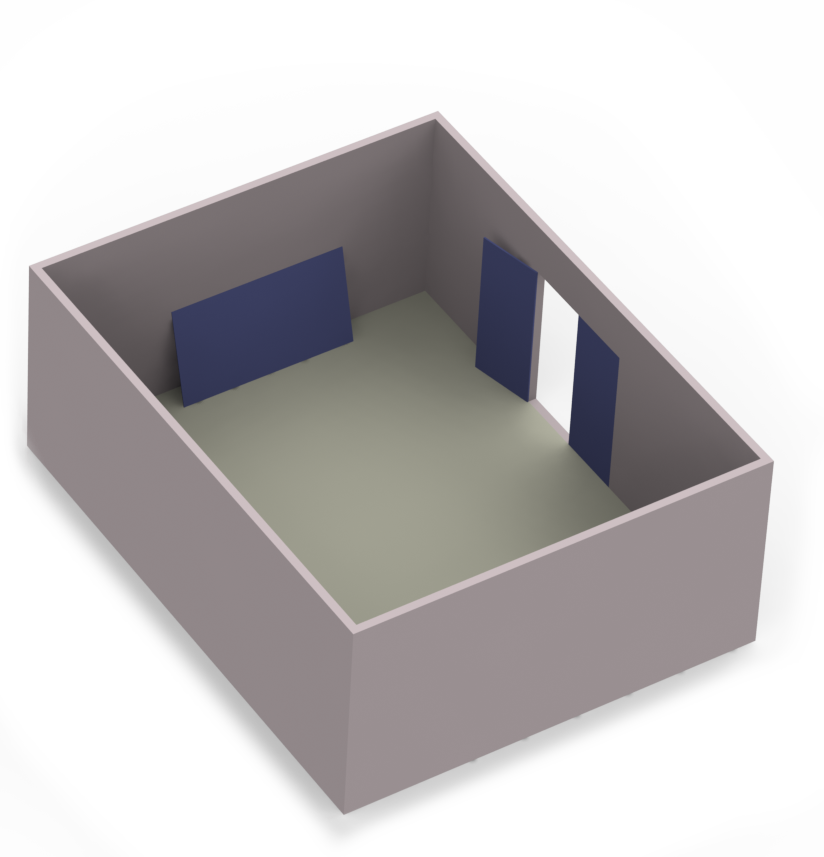
\includegraphics[scale=1.0]{033_cad_02}
		\caption{CAD Modell der Umgebung}
		\label{fig.mapMod}
	\end{center}
	%\vspace*{-8mm}
\end{figure}

Für den Einsatz des \kps{s} ohne vorhandene aktuelle Modelldaten kann eine Kartierung \red[(Mapping)] der Umgebung erfolgen. Die Kartierung von 2D- und 3D-\red[Umge-bungen] ist in aktuellen Forschungen eng mit der Lokalisation innerhalb dieser Umgebungen verknüpft.\red[ Begriff Karte hier einführen?] Ein verbreitetes Forschungsfeld in diesem Zusammenhang ist das simultane Kartieren und Lokalisieren in unbekannten Umgebungen \red[(engl. \textit{Simultaneous Localization And Mapping}, kurz SLAM)]. Dabei existieren verschiedene Algorithmen und Implementierungen zur Lösung der Problemstellungen. Die Kartierung selbst soll in dieser Arbeit nicht näher erläutert werden, für eine detailliertere Darstellung sei deshalb auf \red[\cite{Durrant2006}] verwiesen.\\

Zur Validierung des Systems wurde die in \abb{fig.mapSLAM} dargestellte Umgebung aufgezeichnet. Dabei wurde eine Implementierung \cite{Rgbdslam} nach Endres \textit{et al.} \cite{Endres2014} verwendet, welche die SLAM Anwendung mittels einer RGB-D Kamera realisiert. Das \kps{} kann somit auch für die Kartierung der Umgebung eingesetzt werden.\\

\begin{figure}[ht]
	\begin{center}
		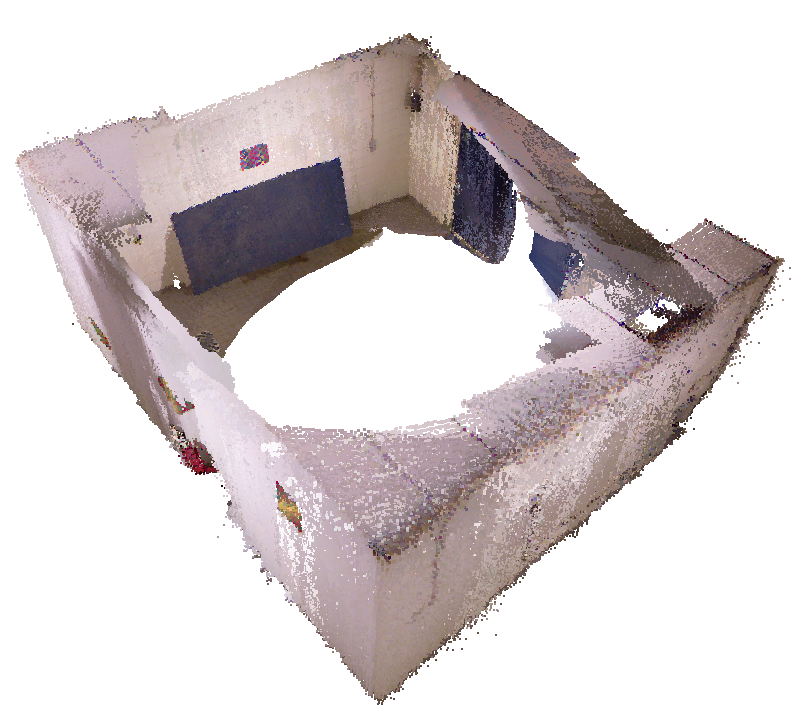
\includegraphics[scale=0.25]{pointcloud_meshlab}
		\caption{Karte RGBDSLAM Subfigures: echter raum (?) - Punktewolke}
		\label{fig.mapSLAM}
	\end{center}
	%\vspace*{-8mm}
\end{figure}

Das Ergebnis der Kartierung entspricht einer texturierten Punktwolke. Im Gegensatz zu der Ableitung aus vorhandenen Modelldaten handelt es sich daher nicht um geschlossene Geometrien. Da die Umgebung selbst jedoch ohnehin nicht als Teil der Projektion eingesetzt wird hat dies keine Auswirkungen auf die Funktionalität des Systems. Nachteiligen Einfluss können jedoch die im Vergleich zu Modelldaten geringere Auflösung sowie die Rauscheinflüsse des Kinect-Sensors zeigen. Die Güte eines Modells aus der Kartierung liegt meist unter der Modellgüte bei Ableitung aus vorhandenen 3D-Daten. Durch Verwendung der selben Sensoren während der Kartierung und der Lokalisation können die Fehlereinflüsse jedoch leicht verringert werden, da wiederkehrende Sensoreinflüsse so bei beiden Verfahren auftreten.\\

\section{Modellobjekte}
Für die Projektion der visuellen Zusatzinformationen sind zu Grunde liegende Modelldaten erforderlich. Modellobjekte beschreiben somit alle Strukturen und Objekte, welche keine Elemente der realen Umgebung abbilden. Die zur Erstellung der Modellumgebung eingesetzten Verfahren können ebenso auf die Modellierung von Objekten und Strukturen angewendet werden. Anstelle von Algortihmen zur Kartierung der Umgebung lassen sich dabei jedoch spezielle Verfahren zur Erfassung dreidimensionaler Objekte einsetzen, wie beispielsweise von Xu \textit{et al.} \cite{Xu2012} beschrieben.\\

Anders als die Modellumgebung müssen die Modellobjekte jedoch nicht als reale Objekte vorhanden sein, weshalb die Modellgüte auch keine Auswirkungen auf die Lokalisations- oder Projektionsgenauigkeit hat. Es können somit beliebige Objekte modelliert werden um diese später in der realen Umgebung zu visualisieren.  Für die Visualisierung ist jedoch eine ausreichende Auflösung der Modellstrukturen und -texturen anzustreben. \abb{fig.modobj} zeigt zwei Beispiele möglicher Modellobjekte und ihre Integration in die Modellumgebung.\\

\begin{figure}[ht]
	\begin{center}
	\subfigure[Modellobjekt Steckdose]{
		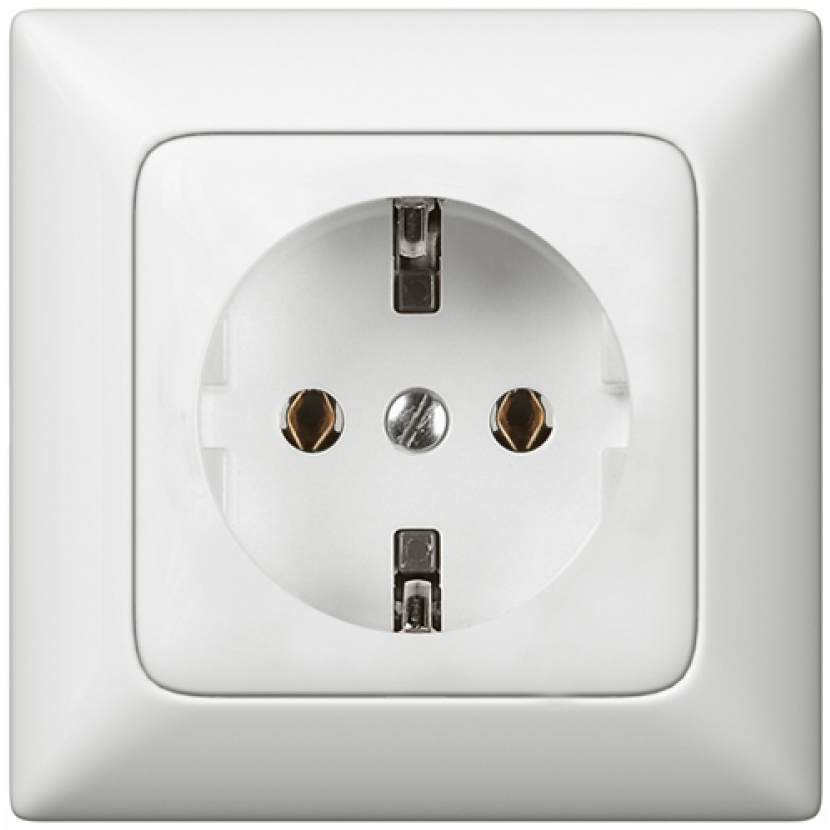
\includegraphics[scale=0.15]{steckdose}
	}
	\hspace{3mm}
%	\subfigure[Modellobjekt elektrische Leitung]{
%			
\includegraphics[scale=1.0]{spacer}
%	}
%	\hspace{3mm}
	\subfigure[Modellobjekte in Modellumgebung]{
		
\includegraphics[scale=1.0]{spacer}
	}
	\caption{Modellobjekte, Subfigures (insgesamt 4, jeweils allein und in Umgebung| Reichen 3? 2xModell + zusammen in Umgebung?): Steckdosen - Leitungen}
	\label{fig.modobj}
	\end{center}
	%\vspace*{-8mm}
\end{figure}

\section{Dateistruktur}
Um die Szene, bestehend aus der Modellumgebung und allen integrierten Modellobjekten, später wieder in den virtuellen Planungsablauf integrieren zu können wird eine Dateistruktur definiert, welche die Sicherung der aktuellen Modellkonfiguration ermöglicht. Alle Modellelement werden dazu mit ihrer aktuellen Pose, Textur und geometrischen Repräsentation erfasst und aufgezeichnet. Eine Wiederherstellung verschiedener Konfigurationen ist damit ebenfalls jederzeit möglich.\\
\red[Dateiformat? YAML? Eine Datei enthält alle Informationen über die Welt und über die einfügbaren Objekte (Preview Funktion). Hinzufügen/entfernen von Objekten zur Datei möglich, suchen nach vorhandenen Objekten in Datenbank möglich?]
	\chapter{Kamera Projektor System}
\red[TODO:\\
Separater Teil?\\
]
\section{Kalibrierung}
Kalibrierung der Kamera. Ergebnis sind Kameraparameter für die RGB und die IR Kamera der Kinect. Dadurch wird die Genauigkeit für die visuelle Odometrie erhöht da die Bilder damit besser aufeinander registriert sind.\\
Kalibrierung des Projektors um die Position bezüglich der Kamera zu bestimmen und um die Perspektive innerhalb des VTK GUIs korrekt abbilden zu können. Beschreibung evtl. unabhängig von der perspektivischen Transformation angeben und nur die allgemeine Transformation beschreiben welche die Bestimmung der Perspektive ermöglicht.

\section{Transformation}
Transformation zwischen den Koordinatensystemen sowohl bezogen auf die Welt bzw. Mapkoordinaten, als auch auf die Transformation zwischen dem Projektor und der Kamera.
    \chapter{Lokalisation}

\section{Lokalisationsverfahren}

\section{Ermittlung der Initialpose}
Globale Lokalisation\\
Für die globale Lokalisation wurde in dieser Arbeit ein Ansatz gewählt, welcher auf dem Monte Carlo Algorithmus basiert. Dieser Ansatz entspricht wie bereits in Kapitel \ref{chap:mcl} beschrieben einem Partikelfilter. In der vorhandenen Umgebungskarte werden im Rahmen zuvor festlegbarer Parameter Partikel basierend auf einer Zufallsverteilung generiert. Jeder Partikel entspricht dabei einer möglichen Pose des Kamera-Projektor-Systems und verfügt demnach über sechs Freiheitsgrade. Die Bestimmung der Pose des Kamera-Projektor-Systems erfolgt durch Auswertung der Partikel basierend auf einer Wahrscheinlichkeitsverteilung. Die Wahrscheinlichkeiten können dabei auf Basis zwei verschiedener Modelle berechnet werden, dem Endpoint-Modell und dem Raycasting-Modell.\\
Beim Endpoint-Modell, welches von X in \cite{Endpoint} beschrieben wurde, erfolgt eine Bestimmung der Wahrscheinlichkeit der Pose basierend auf einem Distanz-Modell, welches für die verwendete Karte statisch ist und damit bereits vor der Lokalisation berechnet werden kann. Dabei wird basierend auf der für die Lokalisation verwendeten Karte eine Lookup-Table erstellt welche die räumlichen Dimensionen der Ausgangskarte abbildet. Jedem Voxel wird dabei ein Distanzwert zugewiesen, basierend auf der Entfernung zum nächsten Hindernis. Als Hindernisse gelten dabei neben dem Raum auch alle statischen Objekte, welche in der Karte vorhanden sind.\\

\begin{figure}[!ht]
	\begin{center}
		
\includegraphics[scale=1.0]{spacer}
		\caption{Distance Map}
		\label{fig.dist_map}
	\end{center}
	%\vspace*{-8mm}
\end{figure}

Durch die vorhergehende Berechnung dieser Karte ergibt sich eine deutliche Verringerung des Rechenaufwands bei jedem Lokalisierungsschritt. Anzumerken bleibt, dass die Distanz-Karte während der gesamten Programmlaufdauer im Speicher behalten wird und bezüglich des Speicherbedarfs die Ausgangskarte deutlich übersteigen kann. Die Lokalisation erfolgt beim beim Endpoint-Modell dann durch Betrachtung der Endpunkte des Tiefenbildes, also der Punkte, welche durch die aufgenommene Punktewolke in Abhängigkeit des betrachteten Partikels innerhalb der Karte abgebildet werden. An diesen Punkten werden die in der zuvor berechneten Distanz-Karte gespeicherten Werte ausgelesen und darauf basierend die Wahrscheinlichkeit berechnet, dass die Punktewolke von der Stelle des betrachteten Partikels aus aufgenommen wurde. Die Berechnung erfolgt mittels der Log-Likelihood-Funktion, welche eine statistische Aussage über die Wahrscheinlichkeit der Messung bestimmt.\\
Beim Raycasting Modell, welches ebenfalls von X in \cite{Raycasting} beschrieben wird, wird für jede Pose eine Betrachtung der Strahlen durchgeführt, welche an dieser Stelle theoretisch in Richtung der Messpunkte ausgesendet werden würden. Entlang dieser Strahlen findet ein Abgleich mit den Daten der Karte statt. Erreicht der Strahl einen besetzen Bereich in der Karte endet die Betrachtung des Strahls an diesem Punkt.\\

\begin{figure}[!ht]
	\begin{center}
		
\includegraphics[scale=1.0]{spacer}
		\caption{Raycasting-Modell}
		\label{fig.raycast}
	\end{center}
	%\vspace*{-8mm}
\end{figure}

Die Entfernung zwischen dem so ermittelten Punkt und dem Betrachteten Partikel wird berechnet und anschließend mit der Entfernung des zugehörigen Sensorwertes verglichen. Die Differenz der beiden Distanzen wird anschließend ermittelt um die Wahrscheinlichkeit zu bestimmen, dass der Sensorwert an dieser Stelle aufgenommen wurde. Die Berechnung der Wahrscheinlichkeit erfolgt dabei ebenfalls mittels der Log-Likelihood-Funktion.\\
\red[LOG-Likelihood Funktion aufführen und beschreiben]

Markerbasierte Lokalisation\\

\section{Verfolgung der aktuellen Pose}
Partikelbasiertes Tracking\\
Featurebasiertes Tracking\\
Beschleunigungsdatenbasiertes Tracking\\
Kombination der Odometriedaten durch Extended Kalman Filter \red[Buch Hertzberg]\\
    \chapter{Visualisierung}
\label{chap.vis}

%PreviewVersion
%\red[TODO:\\
%Ergänzung von Zusatzinformationen noch etwas ausführlicher?\\
%Karte einblenden implementiert?\\
%]

Sobald die aktuelle Position des \kps{s} innerhalb der Umgebung ermittelt wurde kann die Visualisierung der gewünschten Zusatzinformationen basierend auf den Modelldaten (siehe \kapitel{chap.modeldata}) erfolgen. Dieses Kapitel beschreibt das Vorgehen um die ausgewählten Modelldaten mittels des Projektors perspektivisch korrekt in die Umgebung zu projizieren.\\
Zunächst ist die Visualisierung der Modellumgebung und die Ermittlung der Pose des Projektors innerhalb dieser erforderlich. Anschließend erfolgt die Simulation der Projektorsicht durch eine perspektivische Transformation. Die Perspektive wird dabei ausgehend von einem Kameramodell generiert, da der Projektor wie in \abschnitt{chap.kinect} beschrieben als inverse Kamera betrachtet werden kann.\\
Abschließend werden basierend auf der simulierten Perspektive Bilddaten generiert, welche mittels des Projektors für den Anwender und Beobachter innerhalb der realen Umgebung visualisiert werden.

\section{Visualisierung der Modelldaten}
Die Modellumgebung und die Modellobjekte bilden die Grundlage der visuellen Zusatzinformationen die dem Anwender bereitgestellt werden sollen. \\
Um die perspektivische Darstellung zu ermöglichen ist zunächst die gesamte Szene durch die Modelldaten abzubilden. Aufbauend auf der in \kapitel{chap.modeldata} beschriebenen Datenstruktur kann eine Szene erstellt oder geladen und anschließend modifiziert werden. Um eine gerenderte\footnote{Rendern bezeichnet das Ableiten eines Bildes aus virtuellen räumlichen Daten indem die Perspektive eines Beobachters simuliert wird. Dabei können sowohl Lichtverhältnisse als auch Materialeigenschaften berücksichtigt werden um realistische Darstellungen zu erzeugen.} Abbildung der dreidimensionalen Modellszene zu erzeugen wird die Visualisierungsbibliothek VTK (\kapitel{chap.vtk}) verwendet. \abb{fig.modscene} zeigt die Darstellung eines Ausschnitts der Modellszene innerhalb des Visualisierungsbereiches der grafischen Benutzeroberfläche.\\

\begin{figure}[!ht]
	\begin{center}
		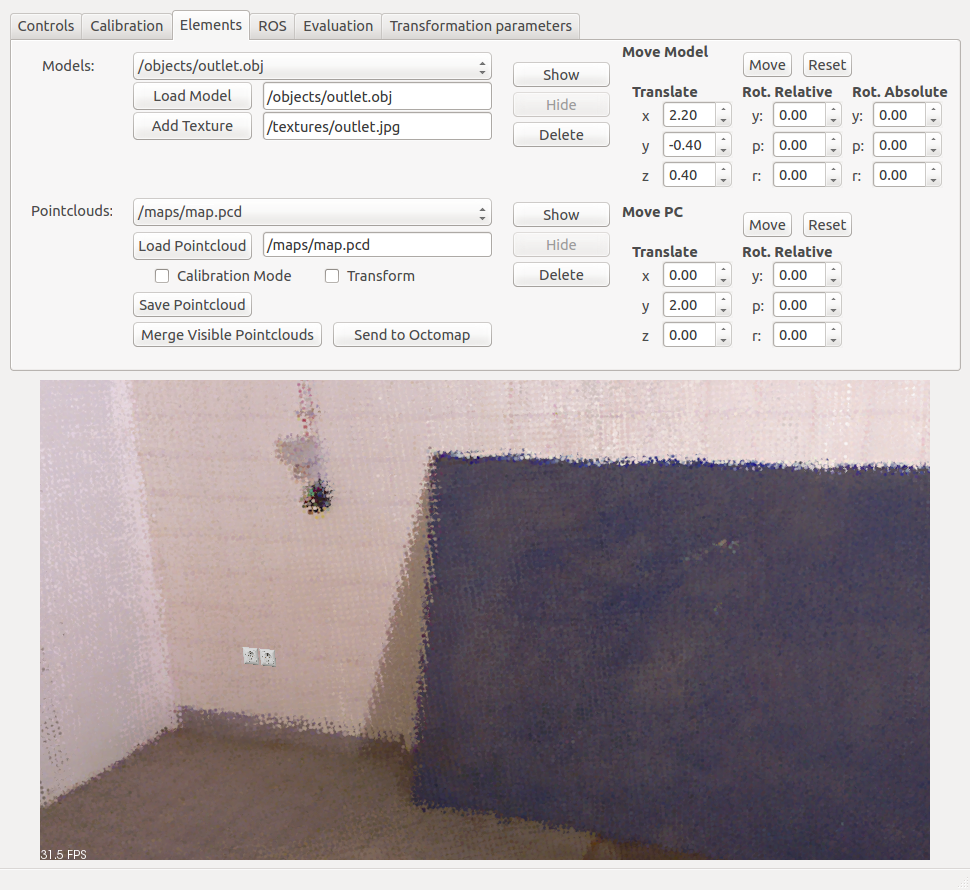
\includegraphics[scale=0.25]{gui}
		\caption{Modellumgebung und Modellobjekte abgebildet innerhalb der grafischen Benutzeroberfläche}
		\label{fig.modscene}
	\end{center}
	%\vspace*{-8mm}
\end{figure}

%PreviewVersion
%\red[CAD-Modell oder Punktwolke? Textur wahrscheinlich schlecht abzubilden!?\\]

Die grafische Benutzeroberfläche ermöglicht die individuelle Positionierung und Ausrichtung aller Elemente. Es werden dadurch die Posen der Objekte und der Umgebung definiert und damit die Transformationen der Modellobjekte $\tmat{0}{Obj}$ und der Modellumgebung $\tmat{0}{Env}$ bezüglich des globalen Koordinatensystems eindeutig festgelegt.\\
Da die für die Lokalisation verwendete Karte aus den Daten der Modellumgebung erzeugt wurde, gilt:

\begin{equation}
\ks{Env} = \ks{M}
\end{equation}

Die Transformation $\tmat{0}{Env}$ ist damit äquivalent zu der Transformation zwischen Karte und globalem Koordinatensystem $\tmat{0}{M}$ und wird deshalb in allen weiteren Ausführungen über diese beschrieben.\\
%PreviewVersion
%Der Zusammenhang zwischen den Koordinaten der Modellumgebung und der Karte der Lokalisation wäre bei einer Veränderung der Pose nicht mehr gegeben und würde zu einem Fehler in der späteren Visualisierung führen. \red[Die grafische Benutzeroberfläche enthält die Möglichkeit eine Zuweisung der Modellelemente zu den Gruppen Umgebung und Objekt vorzunehmen, wodurch die Möglichkeiten zur Modifikation der Elemente entsprechend eingeschränkt oder freigegeben werden.]
%\red[ Objekteigenschaft bool static um Zugehörigkeit zur Map bzw. globalen Koordinaten zu signalisieren. Eigentlich irrelevant in dieser Beschreibung oder?\\]
%\red[Bilder für Modellumgebung und Modellobjekte (z.B. Steckdosen, Leitungen)\\]

\section{Ermittlung der Projektorposition}
Durch die in \abschnitt{chap.projcalib} durchgeführte Kalibrierung ist die externe Transformation $\tmat{KPS}{P}$ zwischen den Basiskoordinaten des \kps{s} und dem Projektor bekannt.\\
Die kontinuierlich durchgeführte Lokalisation des \kps{s} bestimmt die Pose innerhalb der Umgebung worüber sich somit auch die Pose des Projektors bestimmen lässt. Ist diese bekannt, kann durch die Kopplung zwischen den Kartendaten der Lokalisation und den verwendeten Modelldaten die Pose des Projektors innerhalb der simulierten Umgebung bestimmt werden:

\begin{equation}
\tmat{M}{P} = \tmat{M}{Odom}\tmat{Odom}{KPS}\tmat{KPS}{P}
\end{equation}

\section{Perspektivische Transformation}
Die perspektivische Abbildung einer 3D Umgebung auf eine 2D Ebene wurde bereits in \kapitel{chap.perspproj} beschrieben. Der Projektor wird eingesetzt um Daten zu visualisieren, welche zwar innerhalb der Modellumgebung, nicht jedoch in der realen Umgebung vorhanden sind.\\
In der Modellumgebung kann der Projektor deshalb als Kamera simuliert werden, wodurch die Abbildung der Perspektive und Visualisierung dieser möglich wird. Die perspektivische Transformation der Modelldaten erfolgt damit basierend auf der durch die Lokalisation bestimmten extrinsischen $\tmat{M}{P}$ und der bei der Kalibrierung ermittelten intrinsischen Transformation $\tmat{SP}{P}$ des Projektors. Die Abbildung der 3D Modellpunkte auf die 2D pixel der simulierten Kamera wird demnach beschrieben durch:

\begin{equation}
\left(\begin{array}{c}
u_P'\\
v_P'\\
w_P'
\end{array}\right)
= \tmat{SP}{P}(\tmat{M}{P})^{-1}\ve{M}{\tilde{P}} = \tmat{SP}{P}\tmat{P}{M} \left(\begin{array}{c}
X_M\\
Y_M\\
Z_M\\
1
\end{array} \right)
\label{eq.proj_trans}
\end{equation}
%s \cdot \ve{SP}{\tilde{p}} = \tmat{SP}{P}(\tmat{M}{P})^{-1}\ve{M}{\tilde{P}} = \tmat{SP}{P}\tmat{P}{M}\ve{M}{\tilde{P}}

Der durch die Transformation des homogenen 3D-Punktes ermittelte Vektor $[u_P',v_P',w_P']^T$ enthält dabei drei Einträge, welche den in \eq{eq.persp_abb} eingeführten Skalierungsfaktor $s$ enthalten. Um die korrekten Pixelkoordinaten zu ermitteln ist deshalb die Umrechnung der Darstellung des homogenen 2D-Punktes auf einen inversen Streckungsfaktor von $w=1$ erforderlich. Die Pixelkoordinaten des Projektorbildes ergeben sich damit zu:

\begin{equation}
\left(\begin{array}{c}
u_P\\
v_P
\end{array}\right)
=
\left(\begin{array}{c}
\nicefrac{u_P'}{w_P'}\\
\nicefrac{v_P'}{w_P'}
\end{array}\right)
\end{equation}

\abb{fig.projpersp_gui} (a) zeigt die Perspektive des Projektors auf die Modellobjekte innerhalb der Modellumgebung. Bei Generierung der Projektionsabbildung ist zu beachten, dass lediglich die Modellelemente sichtbar sind, die mit dem später projizierten Bild visualisiert werden sollen. Die Modelldaten aller bereits vorhandenen Strukturen werden deshalb wie in \abb{fig.projpersp_gui} (b) gezeigt ausgeblendet, um Überlagerungen von Modelldaten und realen Strukturen zu vermeiden.

%PreviewVersion
%es sei denn, eine   
%optische Bewertung der Projektions- oder Lokalisationsgenauigkeit 
%kann eine Visualiserung der Modellumgebung sinnvoll, um eine  der Überlagerungen von Modelldaten und realen Strukturen zu ermöglichen.

\begin{figure}[!ht]
	\begin{center}
	\subfigure[Projektorperspektive auf Modellumgebung und Modellobjekte]{
		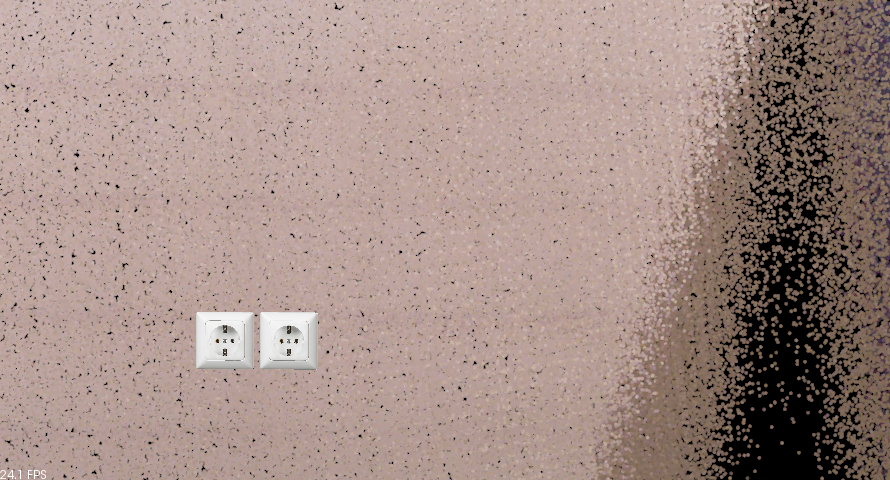
\includegraphics[width=5cm]{proj_persp_incl_map}
	}
	\hspace{5mm}
	\subfigure[Projektorperspektive mit ausgeblendeter Modellumgebung]{
		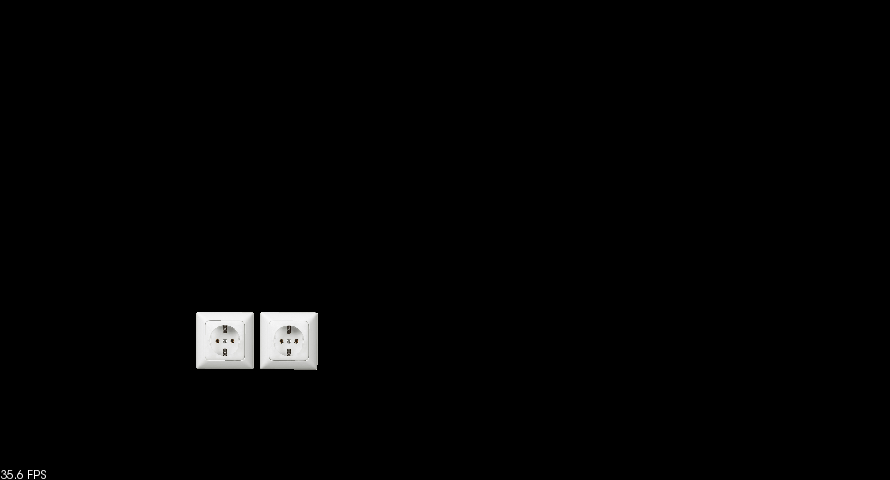
\includegraphics[width=5cm]{proj_persp_no_map}
	}
	\caption{Abbildung der Perspektive des Projektors auf Basis der Modelldaten}
	\label{fig.projpersp_gui}
	\end{center}
	%\vspace*{-8mm}
\end{figure}%
%
%
%\begin{figure}[!ht]
%	\begin{center}
%		\includegraphics[scale=1.0]{perspective_03}
%		\caption{Perspektivische Abbildung der Modelldaten auf die Sensorebene/Pixeldaten des als Kamera simulierten Projektors, grün hervorgehoben das Objekt, das nicht in der Umgebung vorhanden ist aber projiziert werden soll; Rest ausgrauen oder so?}
%		\label{fig.perspproj_vtk}
%	\end{center}
%	%\vspace*{-8mm}
%\end{figure}
%
%\red[Darstellung der Perspektive innerhalb des VTK GUIs]
%
\section{Projektion}
Nachdem durch die perspektivische Transformation ein Bild der Projektorsicht vorliegt erfolgt die Visualisierung der Modellstrukturen in der realen Umgebung. Da bereits alle nötigen Transformationen des Bildes im Rahmen der perspektivischen Abbildung durchgeführt wurden, kann das vorliegende Bild direkt als Ausgangssignal des Projektors verwendet werden.\\
Die Projektion des virtuellen Modellobjektes in die Umgebung ist in \abb{fig.perspproj} dargestellt. 
%zeigt die Abbildung eines Modellobjektes auf die Bildebene des als Kamera simulierten Projektors. 
Die Bildebene wurde dabei zur Verdeutlichung vergrößert innerhalb des Sichtfeldes des Projektors dargestellt. 

\begin{figure}[!ht]
	\begin{center}
		\includegraphics[width=6cm]{perspective_03}
		\caption{Vorgang der Visualisierung von Modelldaten in der Umgebung auf Basis der simulierten Projektorperspektive}
		\label{fig.perspproj}
	\end{center}
	%\vspace*{-8mm}
\end{figure}

Das projizierte Bild muss dabei nicht auf die Visualisierung der Modellobjekte beschränkt werden. Ergänzend kann das Bild mit weitere visuellen Informationen versehen werden. \abb{fig.proj_rms} zeigt, wie das Ausgabebild mit einem Rahmen versehen wurde, welcher dem Anwender eine visuelle Rückmeldung über die Güte der Lokalisation basierend auf dem berechneten QMW (siehe \kapitel{chap.globloc}) gibt.\\

%PreviewVersion
%\red[Projektion der Sicht des Projektors auf das Modell. Ausblenden des Raumes, sodass nur die gewünschten Strukturen dargestellt werden. Alternativ Raummodell als schwarzes Objekt darstellen.\\]

\begin{figure}[!ht]
	\begin{center}
		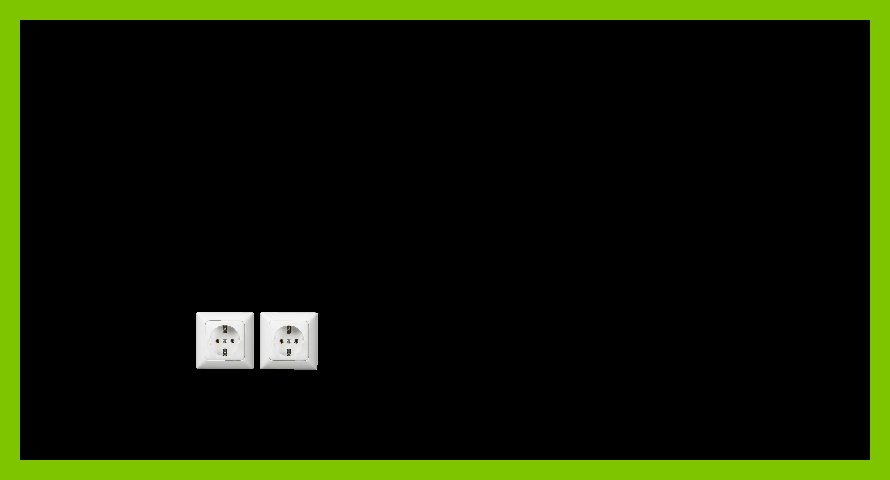
\includegraphics[width=5cm]{proj_persp_frame}
		\caption{Visuelle Rückmeldung für den Anwender über die Lokalisationsgüte}
		\label{fig.proj_rms}
	\end{center}
	%\vspace*{-8mm}
\end{figure}

%PreviewVersion
%\red[Karte einblenden!?]
    \chapter{Interaktion}
\label{chap.interaction}
Um aus der Visualisierung ausgewählter Strukturen und Informationen eine interaktive Projektion zu erzeugen, ist es erforderlich, Benutzereingaben zu erfassen und auszuwerten. Die in diesem Kapitel beschriebene Interaktion ermöglicht dem Benutzer die Projektion und die damit gekoppelten Modelldaten zu modifizieren.

\section{Detektion der Benutzerinteraktion}
Die Erkennung der Benutzereingaben erfolgt durch Auswertung der durch die Kinect gewonnenen Tiefeninformationen in Form der erzeugten Punktwolken. Während der Benutzer das \kps{} in der einen Hand hält, kann die andere Hand verwendet werden, um mit der Projektion zu interagieren. Darüber hinaus ist auch die Interaktion weiterer Benutzer mit dem System möglich.\\
\prever{
%\red[sofern sie bei der Benutzereingabe die Rahmenbedingungen der Funktionsweise beachten].\\
}

Der implementierte Interaktionsansatz basiert auf der Analogie zu einem Laserpointer. Ziel ist es, dem Benutzer durch Zeigebewegungen die Interaktion mit der projizierten Modellumgebung zu ermöglichen. Innerhalb des Softwaremoduls \textit{Interaktion} erfolgt dafür zunächst eine Distanz-Filterung der Punktwolke, da weit entfernte Messpunkte nicht aus der Benutzereingabe stammen können, sondern die Umgebung abbilden. Alle Punkte außerhalb dieses Bereiches können für die weiteren Betrachtungen somit verworfen werden. Es ergibt sich der für die Benutzereingabe zur Verfügung stehende Interaktionsbereich, welcher in \abb{fig.intfov} dargestellt ist.\\
%\red[xmin durch Hardware gegeben, Bereich dann parametrierbar, alles darüber (rot) wird verworfen\\]

\begin{figure}[!ht]
	\begin{center}
		\includesvgnew[1]{images/interaktionsbereich_scaled}%
%		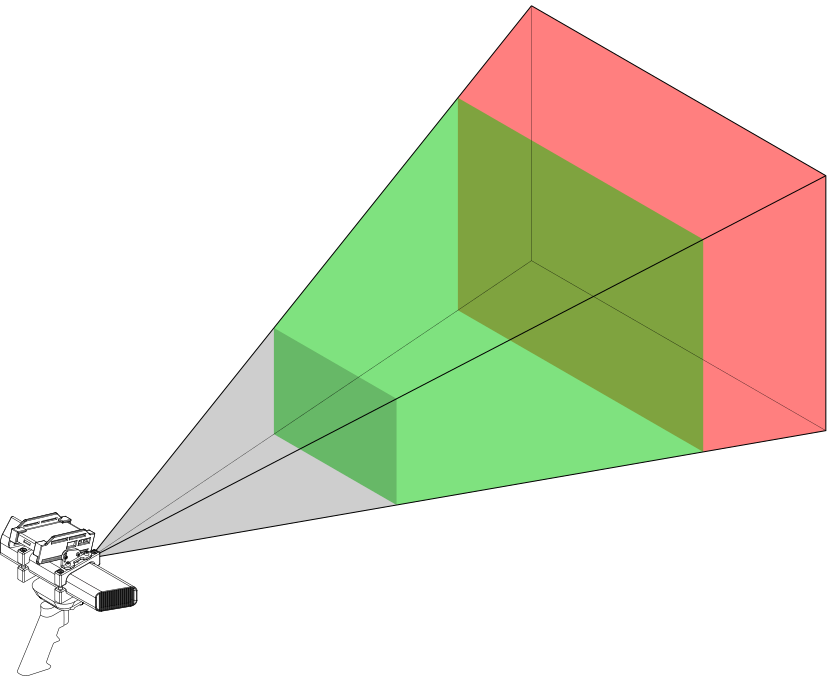
\includegraphics[scale=0.4]{interaktionsbereich}
		\caption{Parametrierbarer Interaktionsbereich}
		\label{fig.intfov}
	\end{center}
	%\vspace*{-18mm}
\end{figure}

\prever{
%\red[Bemaßung!\\]
}
Der minimale Abstand $z_\ind{{min}}$, in welchem Tiefeninformationen ausgewertet werden können, beträgt \SI{0,5}{\meter} und wird durch die Spezifikationen der Kinect definiert. Der maximale Interaktionsabstand $z_\ind{{int}}$ ist im Rahmen der Implementierung parametrierbar und kann damit anwendungsspezifisch definiert werden.\\

\nomenclature[l]{$z_\ind{{min}}$}{Minimal auflösbarer Tiefenwert der Kinect}
\nomenclature[l]{$z_\ind{{int}}$}{Maximaler Tiefenwert des Interaktionsbereichs}


Basierend auf den nach der Filterung verbleibenden Punkten wird eine Ebenendetektion nach \cite{Fischler1981} durchgeführt. Alle Punkte innerhalb eines definierten Abstandes werden daraufhin auf die ermittelte Ebene projiziert, wodurch eine zweidimensionale Abbildung erzeugt und Messwertrauschen geglättet wird. Außerhalb der Ebene liegende Punkte werden für die weiteren Schritte aus der Betrachtung entfernt. Dazu gehören deutliche Ausreißer innerhalb der detektierten Interaktionsstruktur sowie Artefakte in der Punktwolke.\\

Um eine gleichmäßige Objektstruktur zu erhalten wird anschließend eine Hüllkurve um die verbleibenden Punkte gelegt und die vorhandene Struktur mittels einer äquidistanten Verteilung von Punkten angenähert. Aus dieser Hüllkurve wird der geometrische Schwerpunkt (Basis) sowie der vom \kps{} am weitesten entfernte Punkt (Spitze) bestimmt. Der Verbindungsvektor zwischen Basis und Spitze bildet damit die Zeigerichtung des Anwenders ab. Der gesamte Ablauf zur Bestimmung der Zeigerichtung ist in \abb{fig.intdir} dargestellt.\\

\begin{figure}[!ht]
	\begin{center}
	\subfigure[Ausschnitt aus vollständiger Punktwolke]{
		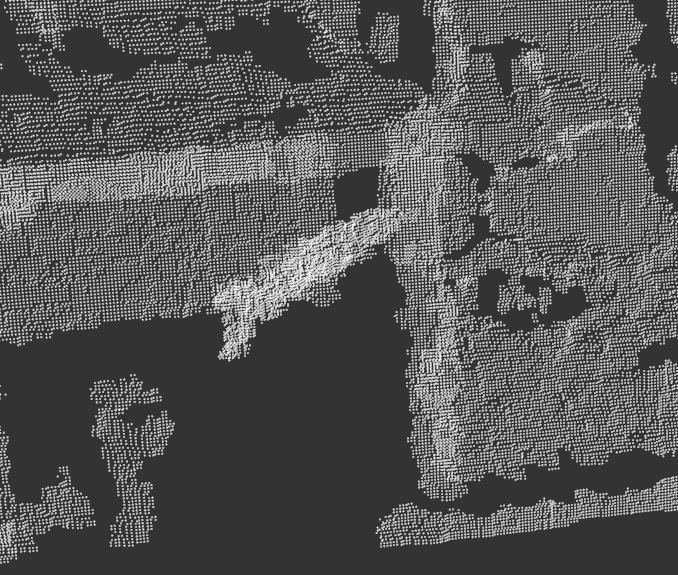
\includegraphics[width=5cm]{interaction_01_02}
	}
	\hspace{5mm}
	\subfigure[Gefilterte Interaktionsstruktur abgebildet auf detektierte Ebene]{
		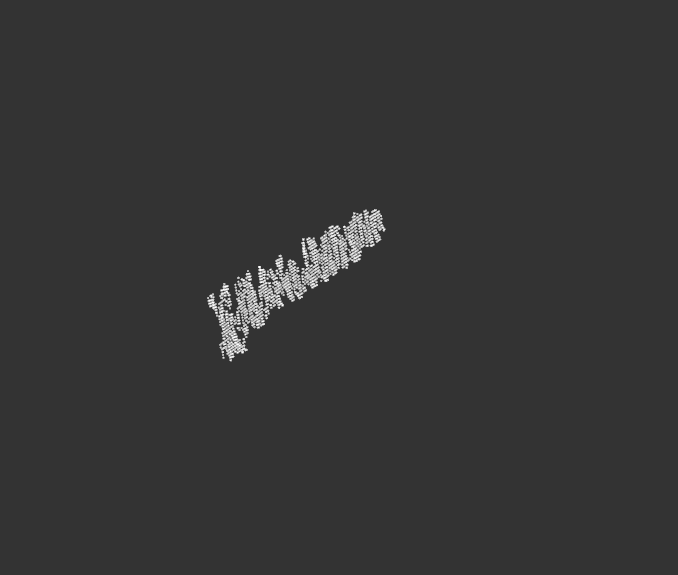
\includegraphics[width=5cm]{interaction_02_02}
	}
		\subfigure[Hüllkurve und geometrischer Schwerpunkt der Struktur]{
		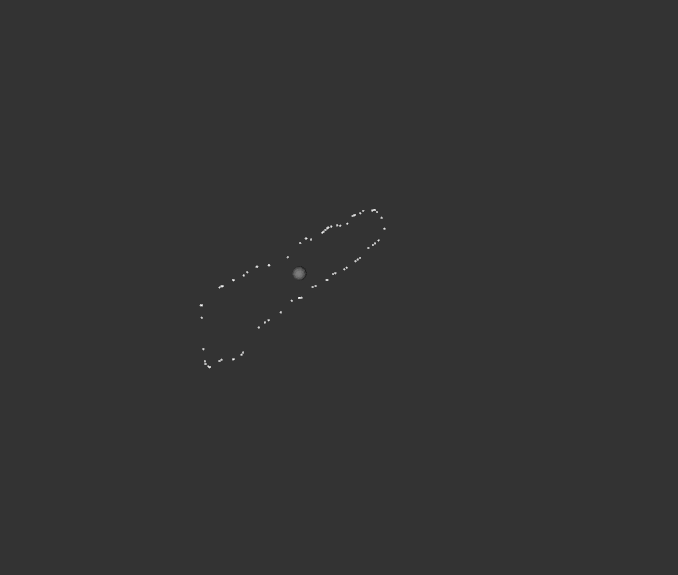
\includegraphics[width=5cm]{interaction_03_02}
	}
	\hspace{5mm}
	\subfigure[Zeigerichtung definiert durch Verbindung zwischen Basis und Spitze]{
		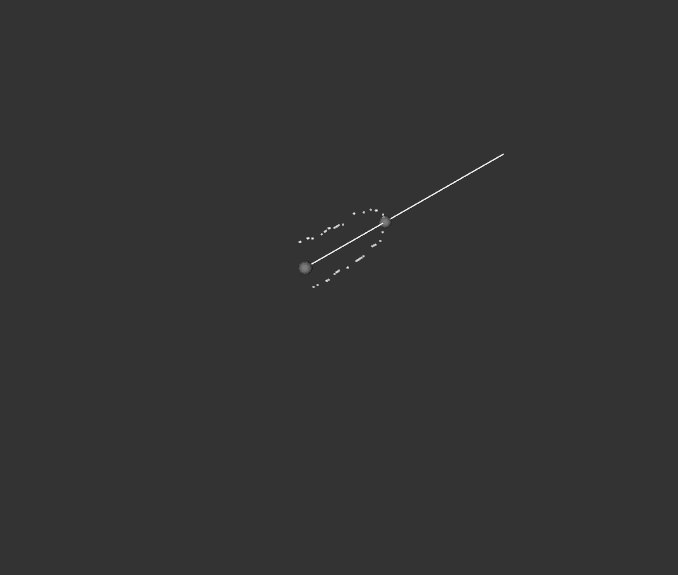
\includegraphics[width=5cm]{interaction_04_02}
	}
	\caption{Filterung der Punktwolke zur Bestimmung der Zeigerichtung}
	\label{fig.intdir}
	\end{center}
	%\vspace*{-8mm}
\end{figure}

Um das Signal der ermittelten Linie zu glätten wird der gleitende Mittelwert der Punkte bestimmt. Auch die Differenz zwischen zwei Punkten aus aufeinander folgenden Messungen wird überwacht, um Sprünge in der Bewegung aufgrund von Fehldetektionen erkennen zu können. Aufgrund des implementierten Ansatzes wurde für die Kommunikation eine Nachrichtenstruktur definiert, welche die erkannte Linie abbildet. Das Modul \textit{Interaktion} stellt die ermittelte Linie über diese Nachricht zur Verfügung, so dass sie vom Softwaremodul \textit{Visualisierung} ausgewertet werden kann.\\

%Da die Kamera des Kinect Sensors auch von dem \mFovis verwendet wird besteht die Gefahr der Beeinflussung zwischen der Benutzereingabe und der lokalen Lokalisation. Um diese zu vermeiden sendet das \mInteraction Modul einen Befehl zum Pausieren der visuellen Odometrie sobald Punkte innerhalb des Interaktionsbereiches erkannt werden. Die visuelle Odometrie wird somit für die Dauer der Benutzerinteraktion unterbrochen. Sobald keine Punkte mehr innerhalb des Interaktionsbereiches detektiert werden, sendet das \mInteraction ein Signal zur Wiederaufnahme der visuellen Odometrie an das \mFovis .

Da die Kamera der Kinect auch zur Bestimmung der visuellen Odometrie verwendet wird, besteht die Möglichkeit, dass die lokale Lokalisation durch die Benutzereingabe beeinträchtigt wird. Um dies zu vermeiden wurde eine direkte Kommunikation zwischen den beteiligten Modulen implementiert. Die Berechnung der visuellen Odometrie wird dabei unterbrochen, sobald Punkte innerhalb des Interaktionsbereiches erkannt werden. Endet die Interaktion, kann die Ermittlung der visuellen Odometrie wieder aufgenommen werden. Im Falle kleiner Posenänderungen während der Benutzereingabe ist die Lokalisation in der Lage die Veränderungen zu erkennen und die Pose im Anschluss an die Benutzerinteraktion zu aktualisieren. Während der Interaktion sollte das Projektionsfeld jedoch ohnehin auf das ausgewählte Objekt ausgerichtet und eine starke Veränderung der Pose des \kps{s} vermieden werden.

\section{Erkennung von Befehlen}
Die Auswertung der auf Basis der Zeigebewegung ermittelten Linie erfolgt innerhalb des Moduls \textit{Visualisierung}. Die Detektion der Linie erfolgte im Koordinatensystem der Kamera $\ks{K}$, so dass diese für die Auswertung zunächst über $\tmat{M}{K}$ in das Koordinatensystem der Karte $\ks{M}$ transformiert wird.\\

Um zu bestimmen, auf welches Modellobjekt der Benutzer gezeigt hat, werden entlang der Linie alle Schnittpunkte mit den virtuellen Modelldaten bestimmt. Dazu wird die Visualisierungsumgebung VTK verwendet, welche die Ermittlung von Schnittpunkten zwischen den Modellobjekten und Linien als Funktion zur Verfügung stellt. Aus den Schnittpunkten kann somit ermittelt werden, welches Objekt der Benutzer ausgewählt hat. Um die Auswahl eines Objektes, analog einer \glqq Klick\grqq -Aktion, zu ermöglichen wurden zwei Verfahren implementiert. Die erste Implementierung erfolgt durch Überprüfung der Verweildauer des simulierten Zeigers auf dem Objekt. Überschreitet diese einen definierten Grenzwert wird dies als Auswahlbefehl gewertet und das Objekt in den Zustand \textit{aktiv} versetzt. Für das zweite Verfahren wurde die Software des Arduino um einen zusätzliche Schnittstelle erweitert. Durch die Anbindung eines Tasters wird die Möglichkeit einer echten \glqq Klick\grqq -Aktion zur Befehlseingabe realisiert. Durch Veränderung der Textur erhält der Anwender wie in \abb{fig.intintersect} dargestellt das visuelle Feedback, dass ein Objekt ausgewählt und in den neuen Status versetzt wurde.\\

\begin{figure}[!ht]
	\begin{center}
	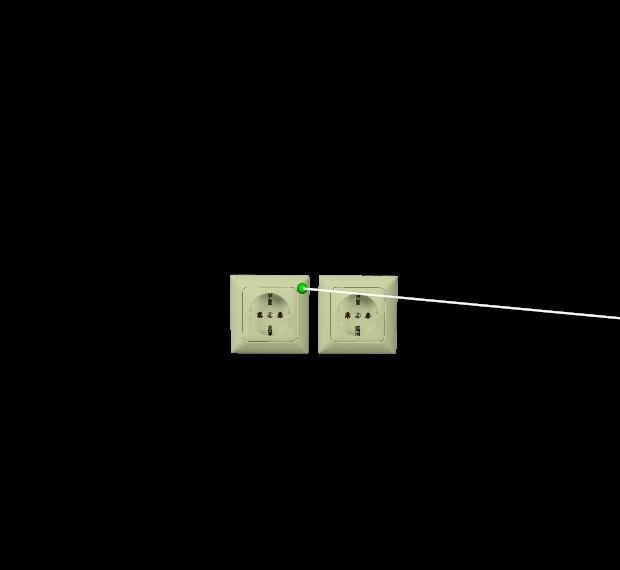
\includegraphics[width=5cm]{model_selection_02}
	\caption{Auswahl eines Modellobjektes durch den Benutzer}
	\label{fig.intintersect}
	\end{center}
	%\vspace*{-8mm}
\end{figure}%

%\begin{figure}[!ht]
%	\begin{center}
%		
\includegraphics[scale=1.0]{spacer}
%		\caption{Subfigures: Line intersection mit Modell und Abbildung des Laserpunktes - Aktivierung des Objektes}
%		\label{fig.intintersect}
%	\end{center}
%	%\vspace*{-8mm}
%\end{figure} 

Innerhalb der Modellumgebung können nun temporäre Interaktionsobjekte wie in \abb{fig.intarrows} (a) dargestellt eingeblendet werden. Über das zuvor beschriebene Funktionsprinzip kann der Benutzer auch diese Objekte auswählen. Alle weiteren Modellobjekte werden während dieser Phase in den Status \textit{inaktiv} versetzt. Es ist somit immer nur ein Objekt der virtuellen Umgebung \textit{aktiv}, wodurch für den Anwender eine klare Zuordnung der Interaktionsobjekte möglich ist. Durch Auswahl der Interaktionsobjekte ist der Benutzer in der Lage das aktuell als \textit{aktiv} gewählte Objekt innerhalb der Modellumgebung zu modifizieren. \abb{fig.intarrows} (b) zeigt dies am Beispiel der Translation des Modellobjektes. Die Anzahl und Funktion der Interaktionsobjekte kann dabei je nach Anwendungsfall spezifiziert werden, so dass eine Modifikation der Objekte bezüglich aller sechs räumlichen Freiheitsgrade möglich ist.\\

\begin{figure}[!ht]
	\begin{center}
	\subfigure[Auswahl eines temporären Interaktionsobjektes]{
		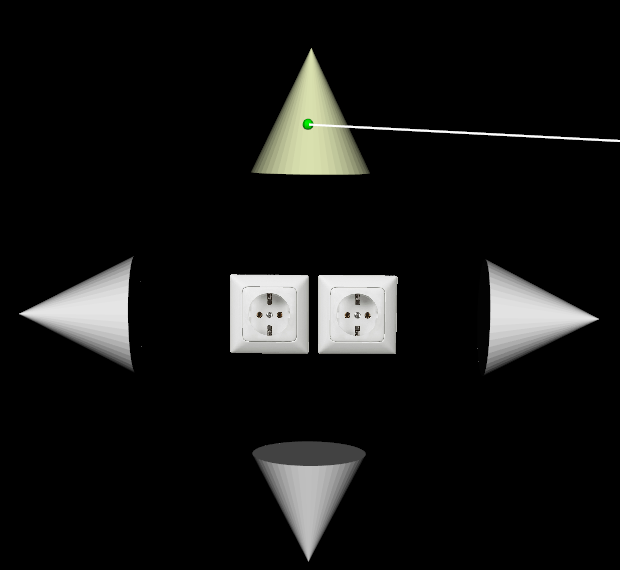
\includegraphics[width=5cm]{model_selection_04}
	}
	\hspace{5mm}
	\subfigure[Bewegtes Modellobjekt mit aktualisierten Interaktionsobjekten]{
		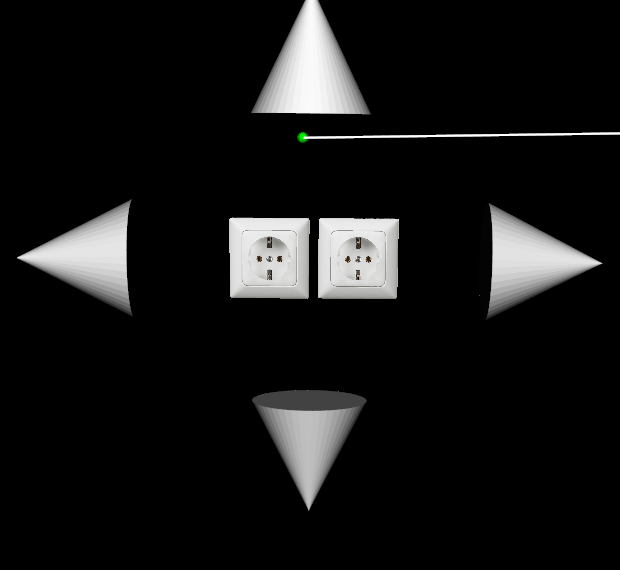
\includegraphics[width=5cm]{model_selection_05}
	}
	\caption{Modifikation der Pose des Modellobjektes durch Auswahl eines Interaktionsobjektes}
	\label{fig.intarrows}
	\end{center}
	%\vspace*{-8mm}
\end{figure}

Durch die Erkennung der Benutzereingabe können somit Objekte der Modellumgebung ausgewählt und bezüglich ihrer Pose modifiziert werden. Die Integration der Interaktion in die Visualisierung ermöglicht die direkte Modifikation der zugrunde liegenden Modelldaten. Das aktualisierte Modell kann abschließend gesichert werden, wodurch eine Rückführung in den virtuellen Modellierungs- und Planungsprozess erreicht wird.

\prever{
%\red[Intersection sollte auch mit Modellumgebung möglich sein, damit der Pointer realistisch abgebildet wird!? Vielleicht Modell (obj) der Karte mit schwarzer Textur?]
}
    \chapter{Datenkopplung}

\section{Modifikation der Modelldaten}
Siehe Kapitel \ref{chap:modell}. An welcher Stelle besser geeignet?

\section{Sichern des aktualisierten Modells}
Siehe Kapitel \ref{chap:modell}. An welcher Stelle besser geeignet?

    \chapter{Limitierungen \red[und Erweiterungen ]des Systems}
Ergänzend zu den zuvor aufgeführten Ergebnissen sollen in diesem Kapitel weitere Fehlereinflüsse und Limitierungen des \kps{s} diskutiert werden. Die vorgestellten Verfahren zur Selbstlokalisation und Darstellung visueller Zusatzinformationen für den Anwender sind allgemein anwendbar und hardwareunabhängig. Wie gezeigt wurde, konnte auf dem verwendeten System ein funktionierender Anwendungsablauf implementiert werden. Eine Erhöhung der Rechenleistung der verwendeten Komponenten würde sich demnach nicht auf das Funktionsprinzip des \kps{s} auswirken, könnte jedoch in verschiedenen Bereichen zu einer \red[Verbesserungen der Performance] führen. Durch den modularen Aufbau der Hard- und Software ist es jederzeit möglich einzelne Komponenten auszutauschen um die Robustheit oder Leistung des Gesamtsystems zu steigern.

\section{Lokalisation}
Eine möglichst präzise Annäherung der tatsächlichen Systempose ist Grundvoraussetzung für die Funktionalität des \kps{s}, da sie sich direkt auf die Projektionsgenauigkeit auswirkt.

Eine allgemeine Limitierung des Kinect Sensors ergibt sich durch das Verfahren zur Ermittlung der Tiefenwerte über die Projektion eines IR-Musters. Eine korrekte Erkennung des Musters kann nur gewährleistet werden, wenn die Beleuchtung der betrachteten Szene keinen \red[starken] IR Anteil aufweist. Insbesondere die Verwendung unter direktem Tageslichteinfall stellt deshalb ein Problem dar. Für den in dieser Arbeit behandelten Anwendungsfall der Lokalisation in geschlossenen Räumen kann dieser Aspekt jedoch vernachlässigt werden.

\subsection{Globale Lokalisation}
Die Auflösung des Kinect Sensors spielt besonders im Rahmen der globalen Lokalisation eine Rolle. Eine höhere Auflösung würde zu einem genaueren Abbild der Umgebung führen. Da vor der Lokalisation jedoch eine Filterung der Punktwolke erfolgt, so dass die Anzahl der betrachteten Punkte verringert wird, wäre ein Zugewinn an Präzision bei aktueller Konfiguration fraglich. Durch \red[Steigerung] der zur Verfügung stehenden Rechenleistung könnte jedoch die gefilterte Auflösung erhöht und die Lokalisationsgenauigkeit und -stabilität verbessert werden.\\

Eine Erhöhung der Rechenleistung könnte darüber hinaus Auch die für die globale Lokalisation benötigte Rechenzeit verringern beziehungsweise die Untersuchung einer größeren Anzahl von Partikeln ermöglichen.\\

\subsection{Visuelle Odometrie}
Das Tracking der Systempose basiert wie beschrieben auf dem Verfahren der visuellen Odometrie. Dazu werden kombinierte Merkmale aus den Aufnahmen der RGB-und IR-Kamera des Kinect Sensors extrahiert. Für eine robuste Bestimmung der Pose ist daher eine hinreichende Anzahl an Merkmalen zu detektieren. Ist die Umgebung nicht ausreichend ausgeleuchtet, können unter Umständen nicht genügend Merkmale bestimmt werden, woraus Fehler in der Lokalisation resultieren. 

\section{Projektion}

\subsection{Microvision ShowWX}
Der ShowWX Laser-Projektor verfügt über eine Helligkeit von etwa 15 Lumen. Dadurch kommt es bei Projektionen in stark ausgeleuchteten Umgebungen und bei größeren Entfernungen zur Projektionsfläche zu einem deutlichen Kontrastverlust.\red[ Bild?] Ein höherer Helligkeitswert würde somit den Anwendungsbereich erweitern. Diese Anforderung steht damit jedoch im Kontrast zu der Anforderung ausreichender Umgebungsausleuchtung für eine robuste visuelle Odometrie. Die Auswirkungen unterschiedlicher Beleuchtungsstärken der Umgebung zeigt \abb{fig.optlight}. Im Anwendungsfall gilt es somit, einen Kompromiss zu finden, welcher beiden Anforderungen gerecht wird.\\
%\red[In Kontrast setzen zu Anforderungen des Projektors -> optimale Helligkeit in der Mitte; Bilder für alle drei Anwendungsfälle aufnehmen?\\]

\begin{figure}[!ht]
	\begin{center}
		
\includegraphics[scale=1.0]{spacer}
		\caption{Optimaler Helligkeitsbereich/Bilder die verdeutlichen wann visodom failt und wann Projektion zu undeutlich wird}
		\label{fig.optlight}
	\end{center}
	%\vspace*{-8mm}
\end{figure}

Anzumerken bleibt, dass eine Begrenzung der Leistung und damit auch der Helligkeit bei Laser-Projektoren durch die zulässige Laser-Klasse vorgegeben ist. Besonders im Bereich der tragbaren Projektoren sollte die Laser-Klasse 2\footnote{Klassifizierung nach EN 60825-1} nicht überschritten werden, da es sonst bei versehentlicher Betrachtung des Laserstrahls zu permanenten Schädigungen der Netzhaut kommen kann. Auch im Hinblick auf die \red[zuvor besprochene] Umgebungsausleuchtung sollte bei der Anwendung deshalb ein maximaler Abstand von etwa \red[TODO] zur Projektionsfläche nicht überschritten werden.\\

Eine weitere Möglichkeit eine deutlichere Darstellung der visuellen Zusatzinformationen zu erreichen, wäre neben einer Kontrast- beziehungsweise Helligkeitserhöhung auch eine Erhöhung der Auflösung der Projektion. Der ShowWX ist auf eine Auflösung von 480p begrenzt, wodurch es besonders bei feineren Strukturen trotz der Laser-Technologie zu unscharfen Abbildungen kommen kann.\\

\subsection{Raspberry Pi}
Für die über den Raspberry Pi realisierte Visualisierung eines \red[ROS-Topics] wurde die Totzeit bestimmt und mit der Ausführung des gleichen Programms auf einem Computer verglichen. Die wichtigsten Spezifikationen der Systeme sind zusammen mit den Ergebnissen der Untersuchung in \tab{totzeit} aufgeführt.

\begin{table}[ht]
\caption{Performance Vergleich zwischen Raspberry Pi und PC}
\begin{center}
\begin{tabular}{|l|c|c|}
\hline
\rowcolor{lightgray} & \multicolumn{1}{|c|}{\textbf{Raspberry Pi}} & \multicolumn{1}{|c|}{\textbf{Computer}}\\
\hline
Taktfrequenz & 700 Mhz & \\
\hline
Kerne & 1 & \\
\hline
Messungen & 20 & 20\\
\hline
Durchschnittliche Totzeit & & \\
\hline
\end{tabular}
\end{center}
\label{tab.totzeit}
\end{table}

Es zeigt sich, \red[TODO]\\
Das gekapselte Projektionsmodul bestehend aus dem Raspberry Pi und dem Microvision ShowWX ist damit \red[nicht geeignet/vergleichbar mit/...]\\
\red[Delay bzgl. raspberry -> Übertragung an anderen Rechner testen und Delay ebenfalls aufzeichnen\\]

\section{Interaktion}
Durch den minimalen aufgelösten Tiefenwert des Microsoft Kinect Sensors von \red[ABSTAND 0,8m?] ergibt sich eine Limitierung der aktuellen Systemkonfiguration bezüglich der Benutzerinteraktion. Um die Zeigerichtung robust erkennen zu können, ist es erforderlich, dass der Nutzer die Auswahl und Modifikation der Modellobjekte mit ausgestrecktem Arm durchführt. Eine kürzere minimale Distanz würde den Komfort bei der Eingabe deutlich erhöhen, da so die Interaktion bei verschiedenen Haltungen möglich wäre und der Benutzer bei längerer Interaktionsdauer entlastet werden würde.\\

Der minimale Tiefenwert definiert darüber hinaus auch den minimalen Abstand zur Projektionsfläche, da sowohl der globalen als auch der lokalen Lokalisation bei Unterschreiten dieses Abstands keine Umgebungsinformationen mehr zur Verfügung stehen. Es ergibt sich daraus zusammen mit dem definierten maximalen Projektionsabstand der in \abb{fig.optdist} dargestellte optimale Anwendungsabstand.\\
\red[Interaktionsbereich hier auch einzeichnen! Wand anstelle rotem Endbereich!?\\]
%\red[Empfehlung für Mindestabstand? Dann auch mit Kinect vergleichen und optimalen Betriebsbereich definieren; Bild, welches diesen darstellt?\\]

\begin{figure}[!ht]
	\begin{center}
		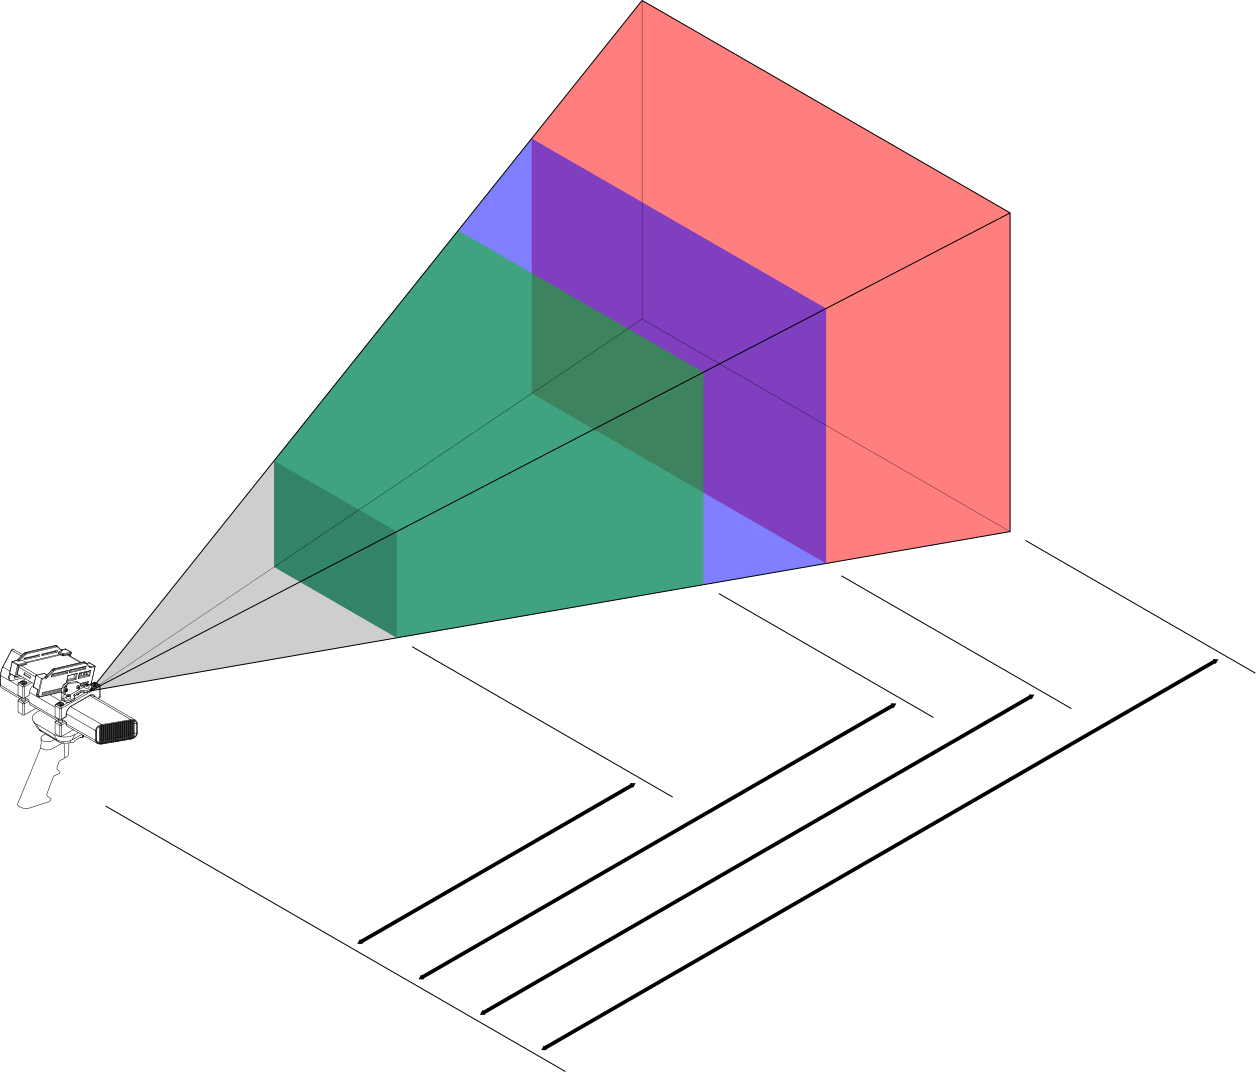
\includegraphics[scale=0.25]{anwendungsbereich}
		\caption{Optimaler Abstand während der Verwendung des \kps{s}}
		\label{fig.optdist}
	\end{center}
	%\vspace*{-8mm}
\end{figure}


%\red[andere Struktur? Nicht Komponenten sondern Lokalisation, Projektion etc.?\\]

\red[TODO:\\
%Einleitender Absatz\\
%Limitierungen der Hardware\\
%Limitierungen der Lokalisation, global und lokal (Licht, features)\\
%Limitierungen des Projektors (Lichtstärke, Auflösung etc.)\\
Limitierungen in der Anwendung\\
Limitierungen in der Rechenleistung\\
]
%\section{Hardware}

%\section{Software}

%\section{Anwendung}
    \chapter{Experimentelle Auswertung und Ergebnisse}
\label{chap.results}
\prever{
%\red[TODO:\\
%PGFPlots einfügen\\
%Daten aufbereiten\\
%Ergebnisse vergleichen/auswerten\\
%Versuchsdurchführungen beschreiben!? Skizzen?\\
%]
}


Um die Funktionalität des \kps{s} bewerten zu können wird eine experimentelle Evaluation durchgeführt. Diese soll besonders dazu dienen, Fehlereinflüsse der aufeinander aufbauenden Transformationen zwischen der Lokalisation des Systems und der Darstellung der visuellen Zusatzinformationen zu quantifizieren. Die Abbildungsgleichung von Punkten der Umgebung auf die Sensorebene des Projektors beschreibt die Verkettung der Transformationen:

\begin{equation}
s \cdot \ve{SP}{\tilde{p}} = \tmat{SP}{P}\cdot\tmat{P}{KPS}\cdot\tmat{KPS}{Odom}\cdot\tmat{Odom}{M}\cdot\tmat{M}{0}\cdot\ve{0}{\tilde{P}}
\end{equation}

Die Karte kann in den Ursprung des globalen Koordinatensystems verschoben werden, wodurch sich $\tmat{M}{0} = \vec{I}$ ergibt. Im Rahmen der globalen Lokalisation wird die Transformation $\tmat{Odom}{M}$ zwischen der Karte und dem Referenz-Koordinatensystem $\ks{Odom}$ ermittelt. Die lokale Lokalisation vervollständigt die Bestimmung der Pose des \kps{s} innerhalb der Karte durch Ermittlung der Transformation $\tmat{KPS}{Odom}$. Die Projektionsgenauigkeit bezogen auf das \kps{} wird abschließend durch die Verknüpfung der extrinsischen $\tmat{P}{KPS}$ und intrinsischen $\tmat{SP}{P}$ Transformationsvorschrift des Projektors beschrieben. Im Folgenden sollen die aufgeführten Transformationen separat betrachtet werden, um die jeweiligen Fehlereinflüsse bestimmen zu können.\\

\prever{
%\red[Gesamte Transformation hier angeben!?\\Globale Lokalisation: Map -> Odom\\Lokale Lokalisation: Odom -> KPS\\Projektionsgenauigkeit: KPS -> Projektor\\]
}
Zunächst erfolgt eine Betrachtung der globalen Lokalisationsgenauigkeit, indem die zwei in \kapitel{chap.globloc} beschriebenen Modelle gegenübergestellt werden. Anschließend wird die Genauigkeit der lokalen Lokalisation bewertet, wobei die visuelle Odometrie und die mittels des EKF fusionierten Sensordaten betrachtet werden. Abschließend wird eine gesonderte Auswertung des Projektionsvorgangs durchgeführt, welcher durch die Transformation zwischen Kamera und Projektor beschrieben wird.\\

Als Bewertungsreferenz der Lokalisation werden die in \abb{fig.armarker} gezeigten Markerfelder verwendet. Durch Erfassung in Kamerabildern können Orientierung und Ursprung der Felder bestimmt werden \cite{arsys}.\\
Je Feld werden vier Marker aufgebracht um die Robustheit der Detektion zu erhöhen. Die Positionierung der Felder ist abhängig von der jeweiligen Untersuchung und wird innerhalb der folgenden Abschnitte detaillierter beschrieben.\\

\begin{figure}[!ht]
	\begin{center}
	
	\subfigure[Markerfeld 1]{
		\begingroup\fboxsep=0pt\fboxrule=1pt
		\fbox{%
			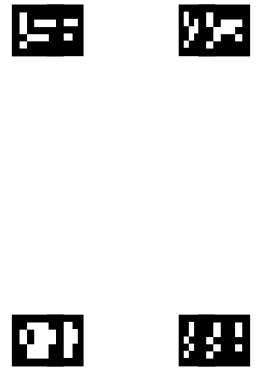
\includegraphics[scale=0.5]{ar_board_01}%
		}
		\endgroup
	}
	\hspace{5mm}
	\subfigure[Markerfeld 2]{
		\begingroup\fboxsep=0pt\fboxrule=1pt
		\fbox{%
			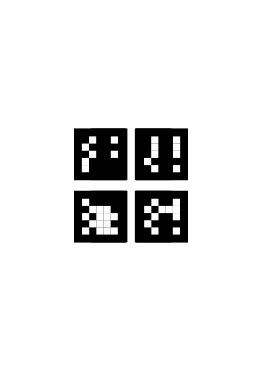
\includegraphics[scale=0.5]{ar_board_02}%	
		}
		\endgroup
	}
	\caption{Markerfelder zur Lagevalidierung}
	\label{fig.armarker}
	\end{center}
	%\vspace*{-8mm}
\end{figure}

Die betrachten Fehlerwerte werden dabei für alle Bewertungen der Lokalisation als Quadratisches Mittel über $k$ Messungen aus den jeweiligen Einzeldifferenzen $r_i$ der Freiheitsgrade der Posen bestimmt:

\begin{equation}
QM = \sqrt{\frac{1}{k} \cdot \sum_{i=1}^kr_i^2}
\end{equation}


\section{Globale Lokalisation}
Die globale Lokalisation bildet die Basis der Lagebestimmung des \kps{s}. Im folgenden werden das RCM und das EPM verglichen und auf ihre Eignung als globales Lokalisationsverfahren des \kps{s} geprüft.\\
Neben der möglichst exakten Annäherung ist dabei auch eine approximative Bestimmung der Systempose von Bedeutung. Wird die Pose innerhalb eines Grenzbereiches angenähert, kann die verbleibende Abweichung durch anschließende Optimierungsschritte verringert werden. Im Falle einer fehlerhaften initialen Lokalisation kann jedoch trotz lokaler Optimierung nicht von einer Verringerung der Abweichung zur wahren Pose ausgegangen werden. Als zusätzliches Bewertungskriterium der globalen Lokalisation wird deshalb im Folgenden neben der Abweichung zur realen Pose auch die Erfolgsquote der Approximation erfasst.\\
Als drittes Vergleichskriterium wird abschließend die für den Lokalisationsvorgang benötigte Rechenzeit ausgewertet.\\

%Dabei ist besonders eine approximative Bestimmung der Systempose von Bedeutung. Die Bestimmung einer möglichst exakten Annäherung der Pose ist zwar prinzipiell ebenso Ziel der globalen Lokalisation, kann jedoch bei korrekter initialer Approximation auch durch anschließende Optimierungsschritte erreicht werden. Im Falle einer fehlerhaften initialen Lokalisation kann trotz einer lokalen Optimierung nicht von einer Verringerung der Abweichung zur wahren Pose ausgegangen werden. Als zusätzliches Bewertungskriterium der globale Lokalisation wird deshalb im Folgenden neben der Abweichung zur realen Pose auch die Erfolgswahrscheinlichkeit der Approximation erfasst.\\

Um die wahre Pose des \kps{s} zu bestimmen wird das Markerfeld innerhalb der realen Umgebung auf einer glatten Fläche befestigt. Der Abgleich zwischen der daraus bestimmten Pose und der durch die Lokalisation ermittelten Pose ist dabei nur möglich, wenn die Pose des Markerfeldes auch in der Modellumgebung bekannt ist. Dies kann entweder durch Anbringung der Markerfelder vor der Kartierung oder durch Definition der Markerpose anhand eindeutiger Landmarken der Umgebung erreicht werden.\\

Die Bestimmung der Referenzpose kann nun durch Erfassung des Markerfeldes mit der Kamera des Systems erfolgen. Dazu wird das \kps{} in einer Pose fixiert und die Transformation $\tmat{MF}{K}$ zwischen dem Markerfeld und der Kamera des \kps{s} bestimmt. Durch die vorhandene Verknüpfung zwischen der realen und der Modellumgebung ist die Transformation $\tmat{M}{MF}$ zwischen den Koordinaten der Karte und dem Markerfeld beschrieben. Ebenso bekannt ist die statische Transformation $\tmat{K}{KPS}$ zwischen der Kamera und dem Basis-Koordinatensystem des \kps{s}. Es lässt sich somit die Transformation zwischen \kps{} und Karte bestimmen zu:

\prever{
\red[Bild für Aufbau?]
}

\begin{equation}
\tmat{M}{KPS} = \tmat{M}{MF} \cdot \tmat{MF}{K} \cdot \tmat{K}{KPS}
\end{equation}

Aus der fixierten Pose wird anschließend die globale Lokalisation durchgeführt. Für beide Modelle werden insgesamt $n=20.000$ Partikel zufällig in der Karte verteilt. Die jeweils ermittelte Pose mit der höchsten Wahrscheinlichkeit wird anschließen mit der Referenzposition verglichen. Dazu wird das quadratische Mittel der Fehler bezüglich der translatorischen ($\Delta X$, $\Delta Y$, $\Delta Z$) und rotatorischen ($\Delta \Psi$, $\Delta \Theta$, $\Delta \Phi$) Freiheitsgrade des Systems bestimmt.\\

In der Fehlerbetrachtung sollen nur die ermittelten Posen berücksichtigt werden, welche eine Annäherung an die tatsächliche Pose innerhalb bestimmter Grenzen darstellen. Außerhalb dieses Bereiches wird von einer fehlerhaften Lokalisation ausgegangen.\\
Um die erfolgreiche Approximation der Pose zu bewerten wird wie in \abb{fig.loclimits} dargestellt deshalb ein Grenzraum um die wahre Position des \kps{s} definiert. Die maximal zulässigen translatorischen und rotatorischen Fehler sind in \tab{thresh_glob} aufgeführt. Die Definition der Grenzwerte erfolgt orientiert an Fehlerwerten, aus welchen in der Literatur die angenäherte Pose optimiert werden konnte \cite{Forster2013}.\\
%\red[Festgelegt nach \cite{Forster2013}\\]

\begin{figure}[!ht]
	\begin{center}
		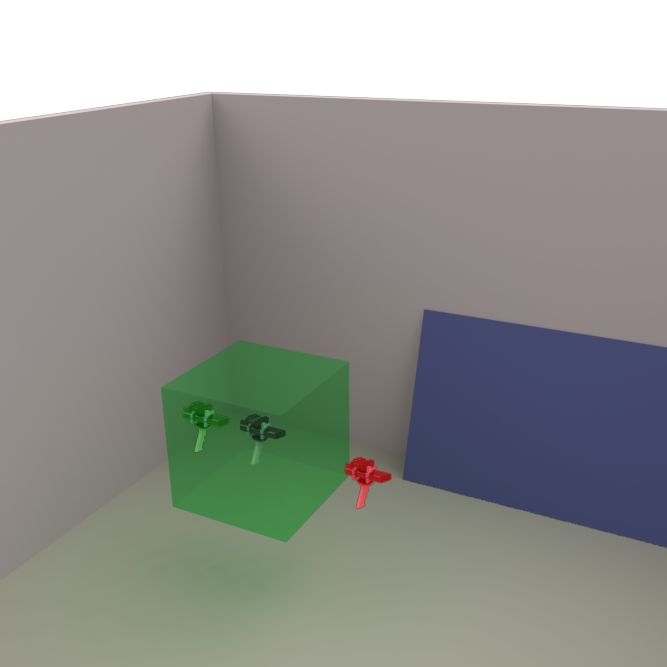
\includegraphics[scale=0.5]{glob_loc_thresh_02}
		\caption{Grenzbereich der Lokalisation mit korrekt angenäherter Pose (grün) und fehlerhafter Lokalisation (rot)}
		\label{fig.loclimits}
	\end{center}
	%\vspace*{-8mm}
\end{figure}

\begin{table}[ht]
	\centering
	\caption{Grenzwerte zur Bestimmung der erfolgreichen Approximation}
	\label{tab.thresh_glob}
	\vspace*{-3mm}
	\begin{tabular}[ht]{|l|r|}\hline
		\rowcolor{Snow2}
		Dimension		& Grenzwert 					\\ \hline
		translatorisch  	& \SI{0,35}{\meter}			\\ \hline
		rotatorisch		& \SI{7}{°}					\\ \hline
%		$X_{lim}$		& \SI{0,35}{\meter}			\\ \hline		
%		$Y_{lim}$		& \SI{0,35}{\meter}			\\ \hline
%		$Z_{lim}$		& \SI{0,35}{\meter}			\\ \hline
%		$\Psi_{lim}$		& \SI{7}{°}					\\ \hline
%		$\Theta_{lim}$	& \SI{7}{°}					\\ \hline
%		$\Phi_{lim}$		& \SI{7}{°}					\\ \hline
	\end{tabular} 
	%\vspace*{-3mm}
\end{table}

Die Erfolgsquote der Annäherung der wahren Systempose berechnet sich aus dem Quotienten der fehlgeschlagenen und insgesamt durchgeführten Lokalisationen. Als fehlgeschlagen werden dabei alle Lokalisationen betrachtet, bei welchen einer der definierten Grenzwerte überschritten wurde. Die Ergebnisse sind zusammen mit der für die globale Lokalisation durchschnittlich benötigten Rechenzeit $\bar{t}$ in \tab{approx_time} aufgeführt.

\begin{table}[ht]
	\centering
	\caption{Ermittelte Erfolgsquote und benötigte Rechenzeit}
	\label{tab.approx_time}
	\vspace*{-3mm}
	\begin{tabular}[ht]{|l|r|r|}\hline
		\rowcolor{Snow2}
		Modell			& Erfolgsquote [$\%$]	&	Rechenzeit $\bar{t}$	 [s]	\\ \hline
		Raycasting		& 56,25					&	\SI{532,89}{}			\\ \hline		
		Endpoint			& 75						&	\SI{55,66}{}			\\ \hline
	\end{tabular} 
	%\vspace*{-3mm}
\end{table}

In der benötigten Rechenzeit zeigt sich deutlich der erwartete höhere Rechenaufwand bei der Verwendung des RCM. Sie beträgt nahezu das \SI{10}{}-fache der für das EPM benötigten Zeit.\\
Die berechnete Erfolgsquote hingegen bestätigt nicht die durch den Rechenaufwand erwartete Genauigkeit des Modells. Nur etwa die Hälfte der Lokalisationsvorgänge des RCM wurde nach den definierten Kriterien als erfolgreich gewertet. Das EPM hingegen schaffte es in zwei drittel der Messungen, die Systempose zu approximieren.\\

%\red[Erfolgsquote interpretieren\\]
%
%Wie aus \tab{approx_time} darüber hinaus ersichtlich wird, beträgt die benötigte Rechenzeit des \red[Raycasting]-Modells fast das \SI{10}{}-fache der vom \red[Endpoint]-Model benötigten Zeit. 
%\red[Zeit der Lokalisation auswerten\\]

Da die Erfolgsquote allein kein ausreichendes Maß darstellt um die Präzision der Annäherung zu bewerten, wird das Quadratische Mittel der Differenzen zwischen tatsächlicher und angenäherter Pose bestimmt. Dabei wurden für jedes Modell $k=12$ gültige Messungen ausgewertet. Die Ergebnisse sind in \abb{fig.glob_loc} in Abhängigkeit des verwendeten Modells aufgeführt.\\

%Auch die globale Lokalisation wird durchgeführt während sich das \kps{} in der fixierten Pose befindet. Für beide Modelle werden insgesamt $n=20.000$ Partikel zufällig in der Karte verteilt. Die jeweils ermittelte Pose mit der höchsten Wahrscheinlichkeit wird anschließen mit der Referenzposition verglichen. Das quadratische Mittel der Fehler aus jeweils \red[$n$] Messungen ist bezüglich der translatorischen ($\Delta X$, $\Delta Y$, $\Delta Z$) und rotatorischen ($\Delta \Psi$, $\Delta \Theta$, $\Delta \Phi$) Freiheitsgrade des Systems sind in \abb{fig.glob_loc} in Abhängigkeit des verwendeten Modells aufgeführt.\\

\prever{
\red[\abb{fig.error_glob_trans} zeigt den Vergleich der durch die beiden Modelle erzielten Fehlerwerte.\\]
\red[Versuchsparameter, Partikelzahl etc.]
}

\begin{figure}
\begin{center}
\begin{tikzpicture}
\tikzstyle{every node}=[font=\small]
\begin{axis}[
	ybar,
	ymax=0.35,
	ymin=0,
	bar width=20pt,
	scaled y ticks = false,
	y tick label style={/pgf/number format/fixed},
%	enlarge y limits={0.4,upper},
	enlarge x limits=0.15,
	legend style={at={(0.5,-0.15)},
	legend style={/tikz/every even column/.append style={column sep=0.5cm}},
	anchor=north,legend columns=-1},
	ylabel={Positionsfehler \lbrack m\rbrack},
%	symbolic x coords={\Delta,y,z},
	xtick={1,2,3,4,5,6},
	xticklabels={$\Delta X$, $\Delta Y$, $\Delta Z$, $\Delta \Psi$, $\Delta \Theta$, $\Delta \Phi$},
%	xtick=data,
	every node near coord/.style={/pgf/number format/fixed,/pgf/number format/use comma, anchor=west},
	nodes near coords,
	nodes near coords align={vertical},
	width=14cm,
	height=8cm,
	grid=major,
    	grid style={dotted,lightgray!80!white},
    	scaled y ticks = false,
]
\addplot[
	every node near coord/.append style={xshift=-0.9cm},
	nodes near coords=\raisebox{0.7cm}{\pgfmathprintnumber\pgfplotspointmeta},
	color=red,
	fill=red!30!white,
	bar shift=-11pt,
] coordinates {(1,0.29) (2,0.24) (3,0.05)};
\addplot[
	every node near coord/.append style={xshift=-0.12cm},
	nodes near coords=\raisebox{0.7cm}{\pgfmathprintnumber\pgfplotspointmeta},
	color=blue,
	fill=blue!30!white,
	bar shift=11pt,	
] coordinates {(1,0.13) (2,0.12) (3,0.03)};
\addplot[fill opacity=0.0,draw=none,] coordinates {(4,0) (5,0) (6,0)};	%dummy
\legend{Raycasting-Modell,Endpoint-Modell}
\end{axis}

\begin{axis}[
%	scale only axis,
	ybar,
	ymax=7,
	ymin=0,
	bar width=20pt,
%	enlarge y limits={0.4,upper},
	enlarge x limits=0.15,
	legend style={at={(0.5,-0.15)},
	anchor=north,legend columns=-1},
	axis y line*=right,
	axis x line=none,
	ylabel={Winkelfehler \lbrack °\rbrack},
%	symbolic x coords={\Delta,y,z},
	xtick={1,2,3,4,5,6},
	xticklabels={$\Delta X$, $\Delta Y$, $\Delta Z$, $\Delta \Psi$, $\Delta \Theta$, $\Delta \Phi$},
%	xtick=data,
%	bar shift=0pt,
	every node near coord/.style={/pgf/number format/fixed,/pgf/number format/use comma, anchor=west},
	nodes near coords,
	nodes near coords align={vertical},
	width=14cm,
	height=8cm,
	grid=major,
    	grid style={dotted,lightgray!80!white},
    	scaled y ticks = false,
]
\addplot[fill opacity=0.0,draw=none,] coordinates {(1,0) (2,0) (3,0)};	%dummy
\addplot[
	every node near coord/.append style={xshift=-0.9cm},
	nodes near coords=\raisebox{0.7cm}{\pgfmathprintnumber\pgfplotspointmeta},
	color=red,
	fill=red!30!white,
	bar shift=-11pt,	
] coordinates {(4,2.44) (5,0.90) (6,5.24)};
\addplot[
	every node near coord/.append style={xshift=-0.12cm},
	nodes near coords=\raisebox{0.7cm}{\pgfmathprintnumber\pgfplotspointmeta},
	color=blue,
	fill=blue!30!white,
	bar shift=11pt,	
] coordinates {(4,3.11) (5,1.59) (6,3.47)};
\end{axis}
\end{tikzpicture}
\end{center}

%\begin{center}
%\begin{tikzpicture}[trim axis left, trim axis right]
%\begin{axis}[
%	ybar,
%	ymax=0.4,
%	ymin=0,
%	bar width=30pt,
%	enlarge x limits=0.4,
%	legend style={at={(0.5,-0.15)},
%	anchor=north,legend columns=-1},
%	ylabel={Positionsfehler \lbrack m\rbrack},
%%	symbolic x coords={\Delta,y,z},
%	xticklabels={$\Delta X$, $\Delta Y$, $\Delta Z$},
%	xtick=data,
%	every node near coord/.style={/pgf/number format/fixed, anchor=west},
%	nodes near coords,
%	nodes near coords align={vertical},
%	width=14cm,
%	height=8cm,
%	grid=major,
%    	grid style={dotted,lightgray!80!white},
%    	scaled y ticks = false,
%]
%\addplot[
%	every node near coord/.append style={xshift=-1.1cm},
%	nodes near coords=\raisebox{0.7cm}{\pgfmathprintnumber\pgfplotspointmeta},
%	color=red,
%	fill=red!30!white
%] coordinates {(-1,0.3105647208) (0,0.3388888731) (1,0.0473358078)};
%\addplot[
%	every node near coord/.append style={xshift=0.0cm},
%	nodes near coords=\raisebox{0.7cm}{\pgfmathprintnumber\pgfplotspointmeta},
%	color=blue,
%	fill=blue!30!white
%] coordinates {(-1,0.1315834135) (0,0.1248760865) (1,0.0209899568)};
%\legend{Raycasting,Endpoint}
%\end{axis}
%\label{fig.error_glob_trans}
%\end{tikzpicture}
%\end{center}
%
%\red[Winkelfehler Vergleich:\\]
%
%\begin{center}
%\begin{tikzpicture}[trim axis left, trim axis right]
%\begin{axis}[
%	ybar,
%	ymax=10,
%	ymin=0,
%	bar width=30pt,
%%	enlarge y limits={0.4,upper},
%	enlarge x limits=0.4,
%	legend style={at={(0.5,-0.15)},
%	anchor=north,legend columns=-1},
%	ylabel={Winkelfehler \lbrack °\rbrack},
%%	symbolic x coords={\Delta,y,z},
%	xticklabels={$\Delta \Psi$, $\Delta \Theta$, $\Delta \Phi$},
%	xtick=data,
%	every node near coord/.style={/pgf/number format/fixed, anchor=west},
%	nodes near coords,
%	nodes near coords align={vertical},
%	width=14cm,
%	height=8cm,
%	grid=major,
%    	grid style={dotted,lightgray!80!white},
%    	scaled y ticks = false,
%]
%\addplot[
%	every node near coord/.append style={xshift=-1.1cm},
%	nodes near coords=\raisebox{0.7cm}{\pgfmathprintnumber\pgfplotspointmeta},
%	color=red,
%	fill=red!30!white
%] coordinates {(-1,2.4445637073) (0,0.9069805767) (1,8.4545773848)};
%\addplot[
%	every node near coord/.append style={xshift=0.0cm},
%	nodes near coords=\raisebox{0.7cm}{\pgfmathprintnumber\pgfplotspointmeta},
%	color=blue,
%	fill=blue!30!white
%] coordinates {(-1,3.1694824628) (0,1.6633422885) (1,4.2398218425)};
%\legend{Raycasting,Endpoint}
%\end{axis}
%\label{fig.error_glob_rot}
%\end{tikzpicture}
%\end{center}


%\begin{figure}[!ht]
%	\begin{center}
%	\subfigure[1. Formparameter (Fokus-Modell)]{
%		\begin{tikzpicture}[scale=0.6, baseline]
%            \begin{axis}[ybar]
%                \addplot+ coordinates {
%                    (1,2)
%                };
%            \end{axis}
%        \end{tikzpicture}
%	}
%	\hspace{2mm}
%	\subfigure[1. Formparameter (Post-Fokus-Modell)]{
%		\begin{tikzpicture}[scale=0.6, baseline]
%            \begin{axis}[ybar]
%                \addplot+ coordinates {
%                    (1,2)
%                };
%            \end{axis}
%        \end{tikzpicture}
%	}\\
%	\caption{Variation der ersten beiden Formparameter um $\pm 3 \sqrt{\lambda_i}$}
%	\label{fig.reference_building_shape_visualization}
%	\end{center}
%	\vspace*{-8mm}
%\end{figure}
\caption{Quadratisches Mittel der Fehlerwerte in der globalen Lokalisation}
\label{fig.glob_loc}
\end{figure}

Die bei der Lokalisation eingesetzte \textit{Octomap} wurde mit einer Auflösung von \SI{0,02}{\meter} aus der vermessenen Umgebung generiert. Diese Unsicherheit ist daher bei der Bewertung der Lokalisationsgüte zu berücksichtigen.\\
Aufgrund der Programmstruktur ist die Vorgabe eines Bereiches zur Verteilung der Partikel bezüglich der Höhe ($z$-Achse des $\ks{M}$) erforderlich. Da das handgeführte \kps{} zu Beginn der Anwendung leicht in einer definierten Höhe gehalten werden kann, wurde dieser Grenzbereich mit einer Toleranz von $\pm$ \SI{0,1}{\meter} zur tatsächlichen Pose definiert. Die Fehlerwerte bezüglich $\Delta Z$ können aufgrund dieser Vorgabe nicht über der gewählten Toleranz liegen.\\
Darüber hinaus verwendet die globale Lokalisation die Daten der inertialen Messeinheit um die Orientierung bezüglich des Roll- ($\Psi$) und Nick-Winkels ($\Theta$) zu bestimmen.\\
Bezüglich dieser drei Freiheitsgrade sind die Fehlerwerte damit nicht abhängig vom verwendeten Modell, wodurch sich die geringeren Differenzen zwischen den Modellen in diesen Bereichen erklären.\\

Für die modellabhängigen Fehlerwerte zeigen sich zwischen dem RCM und dem EPM jedoch deutliche Unterschiede in der Genauigkeit der ermittelten Pose. Die translatorischen Fehlerwerte betragen für das RCM mehr als das doppelte der bei Einsatz des EPM verbleibenden Fehler. Auch in der Bestimmung des Gier-Winkels liegt der Fehlerwert des RCM signifikant über dem des EPM.\\
Wie bereits durch die Erfolgsquote zeigt sich damit, dass das RCM deutlich ungenauere Approximationen der Systempose bestimmt als das EPM.\\

Eine mögliche Ursache dafür liegt in der größeren Toleranz des EPM gegenüber kleineren Abweichungen beim Abgleich zwischen Modell und Messwerten ist. Als Beispiel wird ein Partikel betrachtet, für welches die Messwerte einige Zentimeter in ein Hindernis hinein abgebildet werden. Durch Nichtbeachtung des Strahlenverlaufs unterscheidet sich die Bewertung durch das EPM in diesem Fall nicht von der Bewertung eines Partikels, für welches die Messwerte direkt mit der Außenfläche der Wand abgeglichen werden.\\
Das RCM liefert durch den Abgleich entlang des Sensorstrahls für diese beiden Partikel jedoch deutlich unterschiedliche Fehlerwerte, weshalb das Partikel unter Umständen verworfen wird. Durch Verwendung einer größeren Varianz innerhalb des Sensormodells kann dieser Tatsache zwar entgegengewirkt werden, die Ungenauigkeit in der bestimmten Pose würde sich dadurch jedoch vergrößern.\\

Anzumerken ist, dass aufgrund der Funktionsweise eines Partikelfilters durch Erhöhung der Partikelanzahl das Raster und damit die Auflösung der betrachteten Posen nahezu infinitesimal verfeinert werden kann. Die Durchgeführte Fehlerbetrachtung dient daher insbesondere als Vergleich der beiden Modelle.\\
Die höhere Genauigkeit des EPM in der Approximation zeigt zusammen mit der größeren Erfolgswahrscheinlichkeit und der deutlich geringeren Rechenzeit, dass es für den vorliegenden Anwendungsfall gegenüber dem RCM bevorzugt werden sollte.\\
Die Ungenauigkeiten aufgrund der Funktionsweise des EPM treten in gradlinigen Umgebungen mit geringer Komplexität in den Hintergrund. Da diese Arbeit insbesondere derartige Umgebungen betrachtet, ist das EPM besser als globales Lokalisationsverfahren für diesen Anwendungsfall geeignet als das RCM.

\prever{
%\red[Tiefenauflösung von Distanz abhängig \cite{Khoshelham2012}]
}
%Partikelfilter, deshalb immer Verbesserung theoretisch möglich, bei gleichen Prozessparametern soll jedoch vergleichbarkeit gewährleistet sein. Ziel ist anwendugnsfähiges Modell einzusetzen


%\red[Ergebnisse beschreiben und interpretieren\\]

%\red[Definition, welche als erfolgreich gelten müsste eigentlich vorher schon kommen um daraus die Fehlerwerte zu berechnen!\\]



%\red[Fazit daraus ableiten, welches besser geeignet ist? oder erst im Fazit/Zusammenfassung?\\]


%\red[Quadratischer Mittelwert QMW statt Root Mean Square RMS überall aktualisieren\\]


%\red[Relokalisation bei globaler Lokalisation beschreiben. Besser später als Ergänzung um die lokale Lokalisation zu korrigieren!\\]

\section{Lokale Lokalisation}%Tracking/Kontinuierliche Lokalisation}
Die Genauigkeit der lokalen Lokalisation wird gesondert von der durch die globale Lokalisation bestimmten Pose betrachtet. Dazu wird ebenfalls das für die Untersuchung der globalen Lokalisation verwendete Markerfeld genutzt. Die Referenzpose des Systems kann darüber wie zuvor bestimmt und als Initialisierung der Lokalisation verwendet werden.\\

Zur Bewertung der kontinuierlichen Lokalisation werden translatorische und rotatorische Veränderungen der Systempose vorgenommen. Um eine Beeinflussung der Bewegungen untereinander zu vermeiden erfolgt eine separate Durchführung aller Messungen.\\

\subsection{Translatorische Bewegung}
Die translatorischen Bewegungen werden parallel ($y$-Achse des Systems) und orthogonal ($x$-Achse des Systems) zu der Betrachtungsebene durchgeführt. Die parallele Bewegung entlang der zweiten zur Ebene parallelen Achse ($z$-Achse des Systems) wird nicht gesondert betrachtet, da diese äquivalent zu der Bewegung entlang der ersten ist. \abb{fig.transmove} verdeutlicht dies und zeigt die Durchführung der Untersuchungen anhand eines modellhaften Beispiels des Versuchsaufbaus.\\

\begin{figure}[!ht]
	\begin{center}
		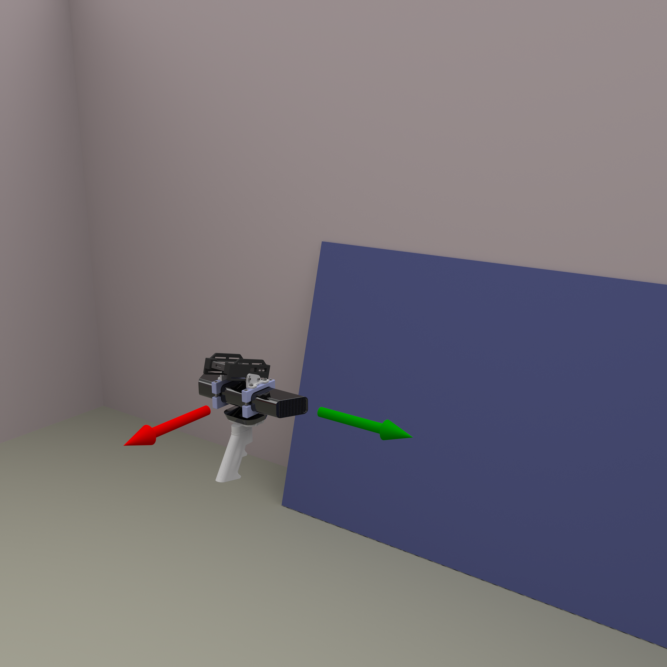
\includegraphics[scale=0.5]{loc_loc_lin}
		\caption{Translatorische Bewegung}
		\label{fig.transmove}
	\end{center}
	%\vspace*{-8mm}
\end{figure}

Bei jeder Messung wird das \kps{} entlang der betrachteten Achse um \SI{1}{\meter} translatorisch verschoben. Insgesamt werden für jede Achse $k=20$ Messungen ausgewertet. Die quadratischen Mittel der Lokalisationsfehler bei translatorischen Bewegungen parallel und orthogonal zur Betrachtungsebene sind in \abb{fig.loc_loc_trans} dargestellt.\\

\begin{figure}
%---------------------------------- Translatorische Bewegung kombiniert in einem Diagramm für alle Freiheitsgrade--------------------------
\begin{center}
\begin{tikzpicture}
\begin{axis}[
	ybar,
	ymax=0.35,
	ymin=0,
	bar width=20pt,
	scaled y ticks = false,
	y tick label style={/pgf/number format/fixed},
%	enlarge y limits={0.4,upper},
	enlarge x limits=0.15,
	legend style={at={(0.5,-0.15)},
	legend style={/tikz/every even column/.append style={column sep=0.5cm}},
	anchor=north,legend columns=-1},
	ylabel={QM der Positionsfehler \lbrack m\rbrack},
%	symbolic x coords={\Delta,y,z},
	xtick={1,2,3,4,5,6},
	xticklabels={$\Delta X$, $\Delta Y$, $\Delta Z$, $\Delta \Psi$, $\Delta \Theta$, $\Delta \Phi$},
%	xtick=data,
%	every node near coord/.style={/pgf/number format/fixed,/pgf/number format/use comma, anchor=west},
%	nodes near coords,
%	nodes near coords align={vertical},
	width=14cm,
	height=8cm,
	grid=major,
    	grid style={dotted,lightgray!80!white},
    	scaled y ticks = false,
]
\addplot[
%	every node near coord/.append style={xshift=-0.9cm},
%	nodes near coords=\raisebox{0.7cm}{\pgfmathprintnumber\pgfplotspointmeta},
	color=Red,
	fill=Red!80!white,
	bar shift=-11pt,
] coordinates {(1,0.22) (2,0.07) (3,0.09)};
\addplot[
%	every node near coord/.append style={xshift=-0.12cm},
%	nodes near coords=\raisebox{0.7cm}{\pgfmathprintnumber\pgfplotspointmeta},
	color=Green,
	fill=Green!60!white,
	bar shift=11pt,	
] coordinates {(1,0.10) (2,0.15) (3,0.07)};
\addplot[fill opacity=0.0,draw=none,] coordinates {(4,0) (5,0) (6,0)};	%dummy
\legend{Translation X,Translation Y}
\end{axis}

\begin{axis}[
%	scale only axis,
	ybar,
	ymax=7,
	ymin=0,
	bar width=20pt,
%	enlarge y limits={0.4,upper},
	enlarge x limits=0.15,
	legend style={at={(0.5,-0.15)},
	anchor=north,legend columns=-1},
	axis y line*=right,
	ylabel={QM der Winkelfehler \lbrack °\rbrack},
%	symbolic x coords={\Delta,y,z},
	xtick={1,2,3,4,5,6},
	xticklabels={},
%	xtick=data,
%	bar shift=0pt,
%	every node near coord/.style={/pgf/number format/fixed,/pgf/number format/use comma, anchor=west},
%	nodes near coords,
%	nodes near coords align={vertical},
	width=14cm,
	height=8cm,
    	scaled y ticks = false,
]
\addplot[fill opacity=0.0,draw=none,] coordinates {(1,0) (2,0) (3,0)};	%dummy
\addplot[
%	every node near coord/.append style={xshift=-0.9cm},
%	nodes near coords=\raisebox{0.7cm}{\pgfmathprintnumber\pgfplotspointmeta},
	color=Red,
	fill=Red!80!white,
	bar shift=-11pt,	
] coordinates {(4,4.73) (5,5.39) (6,4.59)};
\addplot[
%	every node near coord/.append style={xshift=-0.12cm},
%	nodes near coords=\raisebox{0.7cm}{\pgfmathprintnumber\pgfplotspointmeta},
	color=Green,
	fill=Green!60!white,
	bar shift=11pt,	
] coordinates {(4,5.16) (5,4.82) (6,5.75)};
\end{axis}
\end{tikzpicture}
\end{center}

%----------------------------------------------------------------------------------------------------------
%------------------------------------------  Anfang  ------------------------------------------------------
%------------------------ Vergleich mit xyz rpy in getrennten Diagrammen ----------------------------------
%----------------------------------------------------------------------------------------------------------
%----------------------------------------------------------------------------------------------------------
%\subsection{Translatorische Bewegung}
%\begin{center}
%\begin{tikzpicture}[trim axis left, trim axis right]
%\begin{axis}[
%	ybar,
%	ymax=0.25,
%	ymin=0,
%	bar width=30pt,
%	enlarge x limits=0.4,
%	legend style={at={(0.5,-0.15)},
%	anchor=north,legend columns=-1},
%	ylabel={Positionsfehler \lbrack m\rbrack},
%%	symbolic x coords={\Delta,y,z},
%	xticklabels={$\Delta X$, $\Delta Y$, $\Delta Z$},
%	xtick=data,
%	every node near coord/.style={/pgf/number format/fixed, anchor=west},
%	nodes near coords,
%	nodes near coords align={vertical},
%	width=14cm,
%	height=8cm,
%	grid=major,
%    	grid style={dotted,lightgray!80!white},
%    	scaled y ticks = false,
%	y tick label style={/pgf/number format/fixed},
%]
%\addplot[
%	every node near coord/.append style={xshift=-1.1cm},
%	nodes near coords=\raisebox{0.7cm}{\pgfmathprintnumber\pgfplotspointmeta},
%	color=red,
%	fill=red!30!white
%] coordinates {(-1,0.0942737252) (0,0.0744944439) (1,0.2154737652)};
%\addplot[
%	every node near coord/.append style={xshift=0.0cm},
%	nodes near coords=\raisebox{0.7cm}{\pgfmathprintnumber\pgfplotspointmeta},
%	color=blue,
%	fill=blue!30!white
%] coordinates {(-1,0.0141228693) (0,0.0728502984) (1,0.0578491359)};
%\legend{Translatorsich X,Translatorisch Z}
%\end{axis}
%\label{fig.error_glob_trans}
%\end{tikzpicture}
%\end{center}
%
%\begin{center}
%\begin{tikzpicture}[trim axis left, trim axis right]
%\begin{axis}[
%	ybar,
%	ymax=8,
%	ymin=0,
%	bar width=30pt,
%%	enlarge y limits={0.4,upper},
%	enlarge x limits=0.4,
%	legend style={at={(0.5,-0.15)},
%	anchor=north,legend columns=-1},
%	ylabel={Winkelfehler \lbrack °\rbrack},
%%	symbolic x coords={\Delta,y,z},
%	xticklabels={$\Delta \Psi$, $\Delta \Theta$, $\Delta \Phi$},
%	xtick=data,
%	every node near coord/.style={/pgf/number format/fixed, anchor=west},
%	nodes near coords,
%	nodes near coords align={vertical},
%	width=14cm,
%	height=8cm,
%	grid=major,
%    	grid style={dotted,lightgray!80!white},
%    	scaled y ticks = false,
%	y tick label style={/pgf/number format/fixed},    	
%]
%\addplot[
%	every node near coord/.append style={xshift=-1.1cm},
%	nodes near coords=\raisebox{0.7cm}{\pgfmathprintnumber\pgfplotspointmeta},
%	color=red,
%	fill=red!30!white
%] coordinates {(-1,5.3910094725) (0,0.5944624236) (1,4.7266768476)};
%\addplot[
%	every node near coord/.append style={xshift=0.0cm},
%	nodes near coords=\raisebox{0.7cm}{\pgfmathprintnumber\pgfplotspointmeta},
%	color=blue,
%	fill=blue!30!white
%] coordinates {(-1,3.3292065305) (0,1.4935343647) (1,6.1138224963)};
%\legend{Translatorisch X,Translatorisch Z}
%\end{axis}
%\label{fig.error_loc_trans}
%\end{tikzpicture}
%\end{center}
%----------------------------------------------------------------------------------------------------------
%-------------------------------------------  Ende  -------------------------------------------------------
%------------------------ Vergleich mit xyz rpy in getrennten Diagrammen ----------------------------------
%----------------------------------------------------------------------------------------------------------
%----------------------------------------------------------------------------------------------------------

%----------------------------------------------------------------------------------------------------------
%------------------------------------------  Anfang  ------------------------------------------------------
%---------------- Vergleich mit xyz rpy in einem Diagramm, getrennt nach x und z --------------------------
%----------------------------------------------------------------------------------------------------------
%----------------------------------------------------------------------------------------------------------
%\subsection{Translation X}
%\begin{tikzpicture}
%\begin{axis}[
%	ybar,
%	ymax=0.3,
%	ymin=0,
%	bar width=30pt,
%	scaled y ticks = false,
%	y tick label style={/pgf/number format/fixed},
%% 	enlarge y limits={0.4,upper},
%	enlarge x limits=0.2,
%	legend style={at={(0.5,-0.15)},
%	anchor=north,legend columns=-1},
%	ylabel={Positionsfehler \lbrack m\rbrack},
%% 	symbolic x coords={\Delta,y,z},
%	xtick={1,2,3,4,5,6},
%	xticklabels={$\Delta X$, $\Delta Y$, $\Delta Z$, $\Delta \Psi$, $\Delta \Theta$, $\Delta \Phi$},
%% 	xtick=data,
%	bar shift=0pt,
%	every node near coord/.style={/pgf/number format/fixed, anchor=west},
%	nodes near coords,
%	nodes near coords align={vertical},
%	width=14cm,
%	height=8cm,
%	grid=major,
%	grid style={dotted,lightgray!80!white},
%	scaled y ticks = false,
%]
%\addplot[
%	every node near coord/.append style={xshift=-0.55cm},
%	nodes near coords=\raisebox{0.7cm}{\pgfmathprintnumber\pgfplotspointmeta},
%	color=red,
%	fill=red!30!white
%] coordinates {(1,0.0942737252) (2,0.0744944439) (3,0.2154737652)};
%\addplot[fill opacity=0.0,draw=none,] coordinates {(4,0) (5,0) (6,0)}; %dummy
%%\legend{Raycasting,Endpoint}
%\end{axis}
%
%\begin{axis}[
%% 	scale only axis,
%	ybar,
%	ymax=6,
%	ymin=0,
%	bar width=30pt,
%% 	enlarge y limits={0.4,upper},
%	enlarge x limits=0.2,
%	legend style={at={(0.5,-0.15)},
%	anchor=north,legend columns=-1},
%	axis y line*=right,
%	axis x line=none,
%	ylabel={Winkelfehler \lbrack °\rbrack},
%% 	symbolic x coords={\Delta,y,z},
%	xtick={1,2,3,4,5,6},
%	xticklabels={$\Delta X$, $\Delta Y$, $\Delta Z$, $\Delta \Psi$, $\Delta \Theta$, $\Delta \Phi$},
%% 	xtick=data,
%	bar shift=0pt,
%	every node near coord/.style={/pgf/number format/fixed, anchor=west},
%	nodes near coords,
%	nodes near coords align={vertical},
%	width=14cm,
%	height=8cm,
%	grid=major,
%	grid style={dotted,lightgray!80!white},
%	scaled y ticks = false,
%]
%\addplot[fill opacity=0.0,draw=none,] coordinates {(1,0) (2,0) (3,0)}; %dummy
%\addplot[
%	every node near coord/.append style={xshift=-0.55cm},
%	nodes near coords=\raisebox{0.7cm}{\pgfmathprintnumber\pgfplotspointmeta},
%	color=blue,
%	fill=blue!30!white,
%	% fill opacity=0.5,
%	% draw=none,
%] coordinates {(4,5.3910094725) (5,0.5944624236) (6,4.7266768476)};
%\end{axis}
%\label{fig.error_glob_trans_x}
%\end{tikzpicture}
%
%\subsection{Translation Z}
%\begin{tikzpicture}
%\begin{axis}[
%	ybar,
%	ymax=0.2,
%	ymin=0,
%	bar width=30pt,
%	scaled y ticks = false,
%	y tick label style={/pgf/number format/fixed},
%%	enlarge y limits={0.4,upper},
%	enlarge x limits=0.2,
%	legend style={at={(0.5,-0.15)},
%	anchor=north,legend columns=-1},
%	ylabel={Positionsfehler \lbrack m\rbrack},
%%	symbolic x coords={\Delta,y,z},
%	xtick={1,2,3,4,5,6},
%	xticklabels={$\Delta X$, $\Delta Y$, $\Delta Z$, $\Delta \Psi$, $\Delta \Theta$, $\Delta \Phi$},
%%	xtick=data,
%	bar shift=0pt,
%	every node near coord/.style={/pgf/number format/fixed, anchor=west},
%	nodes near coords,
%	nodes near coords align={vertical},
%	width=14cm,
%	height=8cm,
%	grid=major,
%    	grid style={dotted,lightgray!80!white},
%    	scaled y ticks = false,
%]
%\addplot[
%	every node near coord/.append style={xshift=-0.55cm},
%	nodes near coords=\raisebox{0.7cm}{\pgfmathprintnumber\pgfplotspointmeta},
%	color=red,
%	fill=red!30!white
%] coordinates {(1,0.0141228693) (2,0.0728502984) (3,0.0578491359)};
%\addplot[fill opacity=0.0,draw=none,] coordinates {(4,0) (5,0) (6,0)};	%dummy
%%\legend{Raycasting,Endpoint}
%\end{axis}
%
%\begin{axis}[
%%	scale only axis,
%	ybar,
%	ymax=8,
%	ymin=0,
%	bar width=30pt,
%%	enlarge y limits={0.4,upper},
%	enlarge x limits=0.2,
%	legend style={at={(0.5,-0.15)},
%	anchor=north,legend columns=-1},
%	axis y line*=right,
%	axis x line=none,
%	ylabel={Winkelfehler \lbrack °\rbrack},
%%	symbolic x coords={\Delta,y,z},
%	xtick={1,2,3,4,5,6},
%	xticklabels={$\Delta X$, $\Delta Y$, $\Delta Z$, $\Delta \Psi$, $\Delta \Theta$, $\Delta \Phi$},
%%	xtick=data,
%	bar shift=0pt,
%	every node near coord/.style={/pgf/number format/fixed, anchor=west},
%	nodes near coords,
%	nodes near coords align={vertical},
%	width=14cm,
%	height=8cm,
%	grid=major,
%    	grid style={dotted,lightgray!80!white},
%    	scaled y ticks = false,
%]
%\addplot[fill opacity=0.0,draw=none,] coordinates {(1,0) (2,0) (3,0)};	%dummy
%\addplot[
%	every node near coord/.append style={xshift=-0.55cm},
%	nodes near coords=\raisebox{0.7cm}{\pgfmathprintnumber\pgfplotspointmeta},
%	color=blue,
%	fill=blue!30!white,
%%	fill opacity=0.5,
%%	draw=none,
%] coordinates {(4,3.3292065305) (5,1.4935343647) (6,6.1138224963)};
%%\addplot[
%%	every node near coord/.append style={xshift=-1.1cm},
%%	nodes near coords=\raisebox{0.7cm}{\pgfmathprintnumber\pgfplotspointmeta},
%%	color=red,
%%	fill=red!30!white
%%] coordinates {(-2,0) (-1,0) (0,0) (1,2.4445637073) (2,0.9069805767) (3,8.4545773848)};
%\end{axis}
%\label{fig.error_glob_trans_x}
%\end{tikzpicture}
%----------------------------------------------------------------------------------------------------------
%-------------------------------------------  Ende  -------------------------------------------------------
%--------------------------- Vergleich mit xyz rpy in einem Diagramm --------------------------------------
%----------------------------------------------------------------------------------------------------------
%----------------------------------------------------------------------------------------------------------
\caption{Quadratisches Mittel der Fehlerwerte in der lokalen Lokalisation auf Basis der visuellen Odometrie bei translatorischer Bewegung}
\label{fig.loc_loc_trans}
\end{figure}

Beide Messreihen zeigen einen erhöhten Fehlerwert entlang der jeweiligen Translationsrichtung. Die Positionsfehler betragen dabei für die Bewegung parallel zur Betrachtungsebene $15\%$ und für die Bewegung orthogonal zur Betrachtungsebene sogar über $20\%$. Doch auch entlang der zur Translationsrichtung orthogonalen Ebene liegen die Fehlerwerte der Messungen bei etwa $10\%$. Es ergibt sich damit ein deutlicher translatorischer Fehler der durch die visuelle Odometrie bestimmten Pose.\\

Auffällig sind die trotz der rein translatorisch ausgeführten Bewegung hohen Fehler in den ermittelten Achswinkeln. Da sich aus den Ergebnissen kein direkter Zusammenhang mit der Translationsrichtung ableiten lässt, kann von einem grundlegenden Fehler in der durch die visuelle Odometrie ermittelten Orientierung ausgegangen werden.\\
Zur vollständigen Überprüfung sollen dazu im Folgenden die Messungen der rein rotatorischen Bewegungen betrachtet werden.

%\red[Ergebnisse interpretieren\\]
%\red[TransX und TransZ innerhalb vergleichen und Diagramme aufteilen nach translatorischem Fehler und rotatorischem Fehler?\\Oder direkt alles in einem -> 2x6 Balken!?]

\subsection{Rotatorische Bewegung}
%\red[Vergleich zwischen Fovis und Fovis+IMU direkt zusammen in Diagramm aufführen? Erstmal nur Fovis würde dazu dienen, die Bewegungen untereinander zu vergleichen, aber was für Erkenntnisse erhält man daraus? Nick schlechter als Roll ; Nick durch IMU verbessert? -> Kompass sinnvoll! Dann evtl. aber ruhig auch Gierwinkelbewegung aufführen!\\]

Die Lokalisation während der Rotationsbewegungen wird zunächst allein auf Basis der visuellen Odometrie durchgeführt. Analog zur Auswertung der translatorischen Bewegungen werden lediglich die resultierenden Fehler aus den Rotationen um die Roll- und Nick-Achse ausgewertet. Die Rotation des Systems um die Gier-Achse unterscheidet sich für den Algorithmus der visuellen Odometrie nicht von der Rotation um die Nick-Achse, weshalb keine gesonderte Betrachtung durchgeführt wird.\\
Die Versuchsdurchführung der Bewegungen zur Bewertung der rotatorischen Fehlereinflüsse zeigt \abb{fig.rotmove} anhand eines modellhaften Aufbaus.\\

\prever{
%\red[ypr alle aufführen oder nur roll und pitch, da yaw äquivalent zu pitch ist!? s.o.\\]
}

\begin{figure}[!ht]
	\begin{center}
		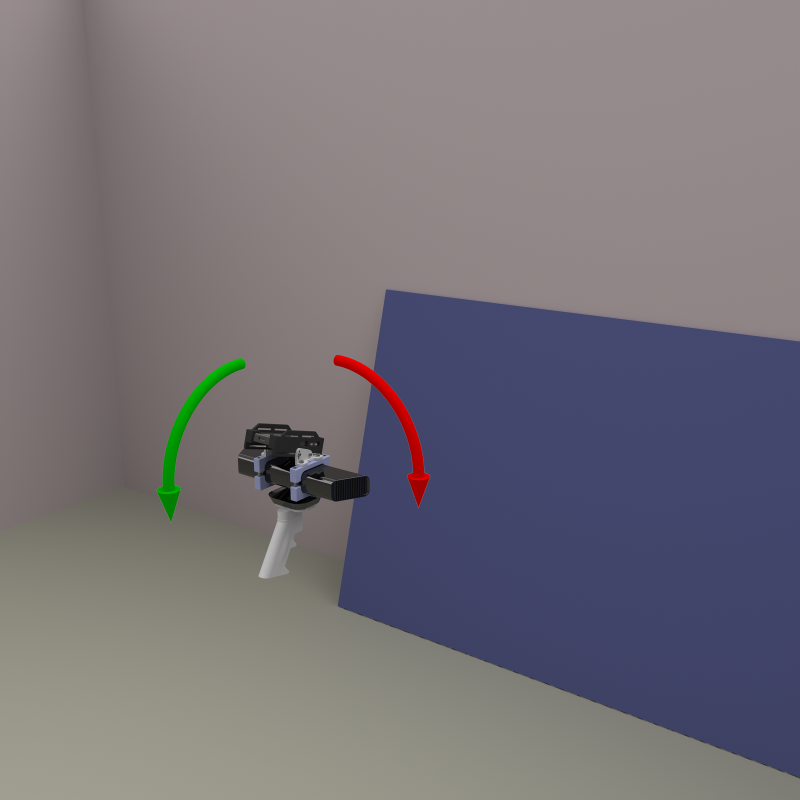
\includegraphics[scale=1]{loc_loc_rot_02}
		\caption{Rotatorische Bewegung}
		\label{fig.rotmove}
	\end{center}
	%\vspace*{-8mm}
\end{figure}

\prever{
%\red[Bilder des Aufbaus als subfigures!?\\]
%\red[Doch nur zwei Freiheitsgrade betrachtet!\\]
}
\prever{
\subsubsection{Visuelle Odometrie}
}
Für alle Messungen wird eine Rotation des \kps{s} von \SI{45}{°} um die betrachtete Achse ausgeführt. Die Quadratischen Mittel der in jeweils $k=20$ Messungen ermittelten Fehler zeigt \abb{fig.loc_loc_rot_fovis}.

\begin{figure}
\begin{center}
\begin{tikzpicture}
\begin{axis}[
	ybar,
	ymax=0.3,
	ymin=0,
	bar width=10pt,
	scaled y ticks = false,
	y tick label style={/pgf/number format/fixed},
%	enlarge y limits={0.4,upper},
	enlarge x limits=0.15,
	legend style={at={(0.5,-0.15)},
	anchor=north,legend columns=-1},
	ylabel={Positionsfehler \lbrack m\rbrack},
%	symbolic x coords={\Delta,y,z},
	xtick={1,2,3,4,5,6},
	xticklabels={$\Delta X$, $\Delta Y$, $\Delta Z$, $\Delta \Psi$, $\Delta \Theta$, $\Delta \Phi$},
%	xtick=data,
%	every node near coord/.style={/pgf/number format/fixed, anchor=west},
%	nodes near coords,
%	nodes near coords align={vertical},
	width=14cm,
	height=8cm,
	grid=major,
    	grid style={dotted,lightgray!80!white},
    	scaled y ticks = false,
]
\addplot[
%	every node near coord/.append style={xshift=-0.95cm},
%	nodes near coords=\raisebox{0.7cm}{\pgfmathprintnumber\pgfplotspointmeta},
	color=red,
	fill=red!30!white,
	bar shift=-12pt,
] coordinates {(1,0.05) (2,0.11) (3,0.26)};
\addplot[
%	every node near coord/.append style={xshift=-0.41cm},
%	nodes near coords=\raisebox{0.7cm}{\pgfmathprintnumber\pgfplotspointmeta},
	color=blue,
	fill=blue!30!white,
	bar shift=0pt,	
] coordinates {(1,0.11) (2,0.21) (3,0.18)};
\addplot[
%	every node near coord/.append style={xshift=0.12cm},
%	nodes near coords=\raisebox{0.7cm}{\pgfmathprintnumber\pgfplotspointmeta},
	color=green,
	fill=green!30!white,
	bar shift=12pt,	
] coordinates {(1,0.21) (2,0.16) (3,0.05)};
\addplot[fill opacity=0.0,draw=none,] coordinates {(4,0) (5,0) (6,0)};	%dummy
\legend{Roll,Pitch,Yaw}
\end{axis}

\begin{axis}[
%	scale only axis,
	ybar,
	ymax=6,
	ymin=0,
	bar width=10pt,
%	enlarge y limits={0.4,upper},
	enlarge x limits=0.15,
	legend style={at={(0.5,-0.15)},
	anchor=north,legend columns=-1},
	axis y line*=right,
	axis x line=none,
	ylabel={Winkelfehler \lbrack °\rbrack},
%	symbolic x coords={\Delta,y,z},
	xtick={1,2,3,4,5,6},
	xticklabels={$\Delta X$, $\Delta Y$, $\Delta Z$, $\Delta \Psi$, $\Delta \Theta$, $\Delta \Phi$},
%	xtick=data,
%	bar shift=0pt,
%	every node near coord/.style={/pgf/number format/fixed, anchor=west},
%	nodes near coords,
%	nodes near coords align={vertical},
	width=14cm,
	height=8cm,
	grid=major,
    	grid style={dotted,lightgray!80!white},
    	scaled y ticks = false,
]
\addplot[fill opacity=0.0,draw=none,] coordinates {(1,0) (2,0) (3,0)};	%dummy
\addplot[
%	every node near coord/.append style={xshift=-0.9cm},
%	nodes near coords=\raisebox{0.7cm}{\pgfmathprintnumber\pgfplotspointmeta},
	color=Red,
	fill=Red!30!white,
	bar shift=-15pt,	
] coordinates {(4,2) (5,2) (6,2)};
\addplot[
%	every node near coord/.append style={xshift=-0.12cm},
%	nodes near coords=\raisebox{0.7cm}{\pgfmathprintnumber\pgfplotspointmeta},
	color=Blue,
	fill=Blue!30!white,
	bar shift=0pt,	
] coordinates {(4,3) (5,3) (6,3)};
\addplot[
%	every node near coord/.append style={xshift=-0.12cm},
%	nodes near coords=\raisebox{0.7cm}{\pgfmathprintnumber\pgfplotspointmeta},
	color=Green,
	fill=Green!30!white,
	bar shift=15pt,	
] coordinates {(4,4) (5,4) (6,4)};
\end{axis}
\label{fig.loc_loc_rot_fovis}
\end{tikzpicture}
\end{center}
\caption{Quadratisches Mittel der Fehlerwerte in der lokalen Lokalisation auf Basis der visuellen Odometrie bei rotatorischer Bewegung}
\label{fig.loc_loc_rot_fovis}
\end{figure}

%\red[Ergebnisse interpretieren\\]

Die Ergebnisse zeigen für alle Achsen einen verbleibenden translatorischen Fehler von unter $10\%$. Die Quadratischen Mittel der rotatorischen Differenzen betragen ebenfalls um $10\%$ und liegen damit nur geringfügig unter den gemessenen Winkelfehlern der translatorischen Bewegungen.\\
Es zeigt sich damit, dass die innerhalb der vorliegenden Rahmenbedingungen über die visuelle Odometrie bestimmten Positionen und Orientierungen unabhängig von der ausgeführten Bewegung mit deutlichen Fehlern behaftet sind.\\

%\red[Allgemein stark abhängig von Features]\\
Eine Erklärung dafür könnte die relativ geringe Anzahl an zuverlässig ermittelten Deskriptoren innerhalb der Kamerabilder sein. Je weniger Merkmale in der Umgebung erkannt werden, desto größer wird der Einfluss fehlerhafter Detektionen auf das Resultat.\\
Die visuelle Odometrie basiert wie in \kapitel{locloc} beschrieben auf dem Abgleich von Merkmalen, welche sich sowohl in den aufgenommen Farb- als auch in den Tiefenwerten wiederfinden. Aus dem Anwendungsziel des \kps{s} ergibt sich insbesondere auch der Einsatz in Umgebungen mit wenigen solcher Merkmale. Auch die experimentelle Auswertung wurde deshalb in einer derartigen Umgebung durchgeführt.\\

Eine weitere Fehlerursache bezüglich der bestimmten Orientierung ergibt sich aus den Anforderungen der verwendeten Implementierung. Diese erfordert eine hohe Frequenz in der Berechnung um Rotationen korrekt anzunähern \cite{Fovis}. Obwohl die Kinect Bilddaten mit einer Rate von \SI{30}{} Bildern pro Sekunde liefert konnten auf dem verwendeten System während der Anwendung nur etwa \SI{5}{} Bilder pro Sekunde ausgewertet werden.\\
Dies ist zum einen auf die Komplexität der Berechnungen zur Bestimmung der visuellen Odometrie und zum anderen auf die hohe Auslastung der Rechenkapazität aufgrund der weiteren verwendeten Softwarekomponenten zurückzuführen.\\ 

%\red[-> Korrektur durch EKF möglich!?\\]
Insgesamt zeigen die Ergebnisse, dass das Verfahren der visuellen Odometrie alleine auf dem verwendeten System nicht in der Lage ist die Veränderungen der Systempose präzise zu bestimmen. Um eine Möglichkeit zur Erhöhung der Robustheit zu betrachten, werden die Untersuchungen der rotatorischen Bewegungen unter Einsatz des EKF wiederholt. Die Daten der visuellen Odometrie werden dabei mit den Lage- und Beschleunigungsdaten der IMU fusioniert.\\

\subsection{Erweitertes Kalman-Filter}
Die Messungen werden auf gleiche Weise wie zuvor durchgeführt. Verglichen werden die Fehler in der ermittelten Systempose auf Basis der visuellen Odometrie und unter Verwendung des EKF. In \abb{fig.loc_loc_rot_ekf_roll} ist der Vergleich bezüglich der Rotation um die Roll- und in \abb{fig.loc_loc_rot_ekf_pitch} bezogen auf die Nick-Achse dargestellt.

%\red[Um die Fusion der Sensordaten mit den Daten der inertialen Messeinheit zu bewerten erfolgt anschließend ein Vergleich mit der Lokalisation auf Basis des Erweiterten Kalman Filters.\\]

\begin{figure}
\begin{center}
\begin{tikzpicture}
\begin{axis}[
	ybar,
	ymax=0.3,
	ymin=0,
	bar width=20pt,
	scaled y ticks = false,
	y tick label style={/pgf/number format/fixed},
%	enlarge y limits={0.4,upper},
	enlarge x limits=0.15,
	legend style={at={(0.5,-0.15)},
	anchor=north,legend columns=-1},
	ylabel={Positionsfehler \lbrack m\rbrack},
%	symbolic x coords={\Delta,y,z},
	xtick={1,2,3,4,5,6},
	xticklabels={$\Delta X$, $\Delta Y$, $\Delta Z$, $\Delta \Psi$, $\Delta \Theta$, $\Delta \Phi$},
%	xtick=data,
	every node near coord/.style={/pgf/number format/fixed, anchor=west},
	nodes near coords,
	nodes near coords align={vertical},
	width=14cm,
	height=8cm,
	grid=major,
    	grid style={dotted,lightgray!80!white},
    	scaled y ticks = false,
]
\addplot[
	every node near coord/.append style={xshift=-0.9cm},
	nodes near coords=\raisebox{0.7cm}{\pgfmathprintnumber\pgfplotspointmeta},
	color=red,
	fill=red!30!white,
	bar shift=-11pt,
] coordinates {(1,0.0942737252) (2,0.0744944439) (3,0.2154737652)};
\addplot[
	every node near coord/.append style={xshift=-0.12cm},
	nodes near coords=\raisebox{0.7cm}{\pgfmathprintnumber\pgfplotspointmeta},
	color=blue,
	fill=blue!30!white,
	bar shift=11pt,	
] coordinates {(1,0.1942737252) (2,0.1744944439) (3,0.1154737652)};
\addplot[fill opacity=0.0,draw=none,] coordinates {(4,0) (5,0) (6,0)};	%dummy
\legend{Rotatorisch Pitch Fovis,Rotatorisch Pitch IMU+EKF}
\end{axis}

\begin{axis}[
%	scale only axis,
	ybar,
	ymax=6,
	ymin=0,
	bar width=20pt,
%	enlarge y limits={0.4,upper},
	enlarge x limits=0.15,
	legend style={at={(0.5,-0.15)},
	anchor=north,legend columns=-1},
	axis y line*=right,
	axis x line=none,
	ylabel={Winkelfehler \lbrack °\rbrack},
%	symbolic x coords={\Delta,y,z},
	xtick={1,2,3,4,5,6},
	xticklabels={$\Delta X$, $\Delta Y$, $\Delta Z$, $\Delta \Psi$, $\Delta \Theta$, $\Delta \Phi$},
%	xtick=data,
%	bar shift=0pt,
	every node near coord/.style={/pgf/number format/fixed, anchor=west},
	nodes near coords,
	nodes near coords align={vertical},
	width=14cm,
	height=8cm,
	grid=major,
    	grid style={dotted,lightgray!80!white},
    	scaled y ticks = false,
]
\addplot[fill opacity=0.0,draw=none,] coordinates {(1,0) (2,0) (3,0)};	%dummy
\addplot[
	every node near coord/.append style={xshift=-0.9cm},
	nodes near coords=\raisebox{0.7cm}{\pgfmathprintnumber\pgfplotspointmeta},
	color=Red,
	fill=Red!30!white,
	bar shift=-11pt,	
] coordinates {(4,5.3910094725) (5,0.5944624236) (6,4.7266768476)};
\addplot[
	every node near coord/.append style={xshift=-0.12cm},
	nodes near coords=\raisebox{0.7cm}{\pgfmathprintnumber\pgfplotspointmeta},
	color=Blue,
	fill=Blue!30!white,
	bar shift=11pt,	
] coordinates {(4,2.3910094725) (5,3.5944624236) (6,1.7266768476)};
\end{axis}
\label{fig.loc_loc_rot_ekf_roll}
\end{tikzpicture}
\end{center}
\caption{Vergleich zwischen den Fehlerwerten der lokalen Lokalisation bei Verwendung der visuellen Odometrie und des EKF. Durchführung einer rotatorischen Bewegung um die Roll-Achse}
\label{fig.loc_loc_rot_ekf_roll}
\end{figure}

\begin{figure}
\begin{center}
\begin{tikzpicture}
\begin{axis}[
	ybar,
	ymax=0.35,
	ymin=0,
	bar width=20pt,
	scaled y ticks = false,
	y tick label style={/pgf/number format/fixed},
%	enlarge y limits={0.4,upper},
	enlarge x limits=0.15,
	legend style={at={(0.5,-0.15)},
	legend style={/tikz/every even column/.append style={column sep=0.5cm}},
	anchor=north,legend columns=-1},
	ylabel={QM der Positionsfehler \lbrack m\rbrack},
%	symbolic x coords={\Delta,y,z},
	xtick={1,2,3,4,5,6},
	xticklabels={$\Delta X$, $\Delta Y$, $\Delta Z$, $\Delta \Psi$, $\Delta \Theta$, $\Delta \Phi$},
%	xtick=data,
%	every node near coord/.style={/pgf/number format/fixed,/pgf/number format/use comma, anchor=west},
%	nodes near coords,
%	nodes near coords align={vertical},
	width=14cm,
	height=8cm,
	grid=major,
    	grid style={dotted,lightgray!80!white},
    	scaled y ticks = false,
]
\addplot[
%	every node near coord/.append style={xshift=-0.9cm},
%	nodes near coords=\raisebox{0.7cm}{\pgfmathprintnumber\pgfplotspointmeta},
	color=red,
	fill=red!50!white,
	bar shift=-11pt,
] coordinates {(1,0.04) (2,0.09) (3,0.06)};
\addplot[
%	every node near coord/.append style={xshift=-0.12cm},
%	nodes near coords=\raisebox{0.7cm}{\pgfmathprintnumber\pgfplotspointmeta},
	color=blue,
	fill=blue!50!white,
	bar shift=11pt,	
] coordinates {(1,0.07) (2,0.06) (3,0.05)};
\addplot[fill opacity=0.0,draw=none,] coordinates {(4,0) (5,0) (6,0)};	%dummy
\legend{Nicken - Visuelle Odometrie,Nicken - EKF}
\end{axis}

\begin{axis}[
%	scale only axis,
	ybar,
	ymax=7,
	ymin=0,
	bar width=20pt,
%	enlarge y limits={0.4,upper},
	enlarge x limits=0.15,
	legend style={at={(0.5,-0.15)},
	anchor=north,legend columns=-1},
	axis y line*=right,
	ylabel={QM der Winkelfehler \lbrack °\rbrack},
%	symbolic x coords={\Delta,y,z},
	xtick={1,2,3,4,5,6},
	xticklabels={$\Delta X$, $\Delta Y$, $\Delta Z$, $\Delta \Psi$, $\Delta \Theta$, $\Delta \Phi$},
%	xtick=data,
%	bar shift=0pt,
%	every node near coord/.style={/pgf/number format/fixed,/pgf/number format/use comma, anchor=west},
%	nodes near coords,
%	nodes near coords align={vertical},
	width=14cm,
	height=8cm,
    	scaled y ticks = false,
]
\addplot[fill opacity=0.0,draw=none,] coordinates {(1,0) (2,0) (3,0)};	%dummy
\addplot[
%	every node near coord/.append style={xshift=-0.9cm},
%	nodes near coords=\raisebox{0.7cm}{\pgfmathprintnumber\pgfplotspointmeta},
	color=red,
	fill=red!50!white,
	bar shift=-11pt,	
] coordinates {(4,3.39) (5,4.29) (6,4.70)};
\addplot[
%	every node near coord/.append style={xshift=-0.12cm},
%	nodes near coords=\raisebox{0.7cm}{\pgfmathprintnumber\pgfplotspointmeta},
	color=blue,
	fill=blue!50!white,
	bar shift=11pt,	
] coordinates {(4,2.18) (5,1.64) (6,3.75)};
\end{axis}
\end{tikzpicture}
\end{center}
\caption{Vergleich zwischen den Fehlerwerten der lokalen Lokalisation bei Verwendung der visuellen Odometrie und des EKF. Durchführung einer rotatorischen Bewegung um die Nick-Achse}
\label{fig.loc_loc_rot_ekf_pitch}
\end{figure}

%\red[Ergebnisse interpretieren\\]

In beiden Messreihen zeigen sich deutliche Auswirkungen auf die Freiheitsgrade, für welche die IMU Lagedaten bereitstellt. Die Fusion der Sensorwerte führt zu einer starken Verringerung der Fehler in der Winkelbestimmung bezüglich der Roll- und Nick-Achse.\\
Die Genauigkeit der Lokalisation während der kontinuierlichen Bestimmung der Pose konnte damit für zwei der sechs Freiheitsgrade erhöht werden.\\

Um die Fehlerfortpflanzung im Verlauf der lokalen Lokalisation zu verringern wurde die Implementierung der globalen Lokalisation um zusätzliche Funktionalität erweitert. Dabei wird die Ausführung einer modifizierten Variante der globalen Lokalisation ermöglicht.\\
In einem definierten Parameterbereich werden Partikel um die aktuelle Pose gestreut, so dass das lokale Optimum neu ermittelt wird. Die verwendete Anzahl Partikel kann dabei geringer gewählt werden als bei der globalen Lokalisation, wodurch dieser Schritt mit deutlich geringerer Rechenzeit verbunden ist. Diese Funktion kann automatisch oder manuell durch den Benutzer aufgerufen werden, so dass zu definierten Zeitpunkten eine Korrektur der ermittelten Pose erzielt wird. Dabei ermöglicht die in \kapitel{chap.projection} beschriebene visuelle Rückmeldung über den aktuellen Überdeckungsfehler eine direkte Bewertung der korrigierten Pose.

%\red[Globale Lokalisation mit weniger Partikel als lokale Lokalisation verwenden! -> Hier aufführen? Ohne Messungen?]

\prever{
\red[(englisch inertial measurement unit, IMU) -> IMU überall ersetzen\\]
}
%\subsection{Rotation Roll IMU+KALMAN}


%\red[Mögliche Lösungsansätze hier thematisieren?\\] 

\section{Visualisierung}
Um die präzise Abbildung der visuellen Zusatzinformationen in der realen Umgebung zu ermöglichen ist über die Lokalisation hinaus auch eine hohe Genauigkeit der Projektion erforderlich. Die Interaktion des Benutzers mit der Projektion erfordert zudem eine dynamische Darstellung mit geringer Verzögerung\\
Im Folgenden soll deshalb im Rahmen experimenteller Untersuchungen zunächst die Projektionsgenauigkeit und abschließend die Latenzzeit der Visualisierung ermittelt werden.

\subsection{Projektionsgenauigkeit}
Die Genauigkeit der Projektion virtueller Modelldaten wird unter Verwendung einer externen Kamera analysiert. Diese wird zunächst analog zu dem in \kapitel{chap.calib} beschriebenen Vorgehen für die RGB-Kamera der Kinect kalibriert, wodurch eine objektive Betrachtung der Projektionsgenauigkeit ermöglicht wird. Für die Untersuchung wird ein Markerfeld auf einer ebenen Unterlage fixiert und im Sicht- und Projektionsfeld des \kps{s} platziert. Das Markerfeld wird mittels der RGB-Kamera der Kinect erfasst, um die Transformation des \kps{s} relativ zum Markerfeld zu bestimmen.\\

Die bekannte Transformation zwischen Kamera- und Projektorkoordinaten ermöglicht daraufhin die Zuordnung der detektierten 3D-Koordinaten des Markerfeldes zu den 2D-Koordinaten des Projektorbildes. Um die Projektionsgenauigkeit zu überprüfen wird mittels des Projektors ein weiteres Markerfeld projiziert, welches bezogen auf die Projektorkoordinaten deckungsgleich mit dem realen Markerfeld ist. Dazu werden beide Markerfelder in der Modellumgebung dargestellt und überlagert. Die externe Kamera wird anschließend so positioniert, dass sie in der Lage ist das reale und das projizierte Markerfeld zu erfassen. Es ergibt sich daraus der in \abb{fig.arprojected} dargestellte Versuchsaufbau.\\

\begin{figure}[ht]
	\begin{center}%
		\includesvgnew[1]{images/projection_validation_cropped}%
		\caption{Aufbau zur Überprüfung der Projektionsgenauigkeit}
		\label{fig.projsetup}
	\end{center}
	%\vspace*{-8mm}
\end{figure}
%\red[Projiziertes Feld: Kästchen entfernen!\\]

Durch Detektion der Markerfelder im Bild der externen Kamera können wie in \abb{fig.projsetup} ihre Posen ermittelt werden. Aus der relativen Transformation zwischen den Feldern lassen sich die Abweichungen bezüglich Position und Orientierung bestimmen. Sowohl die Positionierung des \kps{s} als auch der externen Kamera wird dabei während der Untersuchungen variiert.\\

\begin{figure}[!ht]
	\begin{center}
		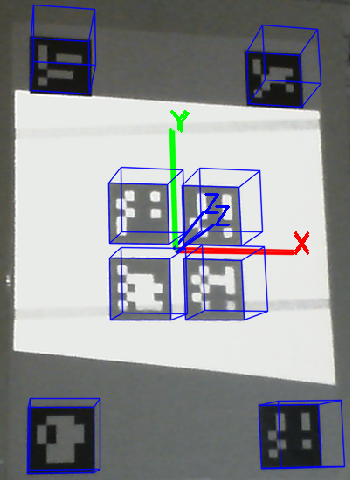
\includegraphics[scale=0.4]{board_eval_cropped}
		\caption{Detektion des realen und projizierten Markerfeldes im Bild der externen Kamera}
		\label{fig.arprojected}
	\end{center}
	%\vspace*{-8mm}
\end{figure}

Die relativen Fehler der $n=6$ Messreihen mit insgesamt $k=229$ Messungen sind als Box-Whisker-Plot in \abb{fig.boxplot_proj} dargestellt. Dabei wurde die Gesamtheit der Messwerte in die Darstellung aufgenommen. Die farbliche Abbildung der Messungen dient der besseren Übersicht und wurde in Orientierung an die verwendete RGB-Darstellung der Koordinatensysteme gewählt.

\begin{figure}[!ht]
\begin{center}
\begin{tikzpicture}[trim axis left, trim axis right]
  \begin{axis}[
    	ytick={-30,-20,...,30},
    		minor y tick num=1,
    		ymax=35,
    		ymin=-35,
    		ylabel=Positionsfehler \lbrack mm\rbrack,
    		xtick={1,2,...,6},
    		x tick label style={align=center},
    		xticklabels={$\Delta X$, $\Delta Y$, $\Delta Z$, $\Delta \Psi$, $\Delta \Theta$, $\Delta \Phi$},
    		boxplot/draw direction=y,
    		width=14cm,
    		height=8cm,
    		grid=major,
    		grid style={dotted,lightgray!80!white},
    ]
    \addplot+[color=red,mark=x,
    		boxplot prepared={
      		lower whisker=-7.2937458753,
      		lower quartile=-2.2697057575,
      		median=-0.5078930408,
      		upper quartile=2.5787912309,
      		upper whisker=5.2836090326,
      		box extend=0.5,
      		draw position=1,
    		},
    ] coordinates {};
    %table[row sep=\\,y index=0] {0.0\\}; %Ausreisser
    \addplot+[color=Green,mark=x,
    		boxplot prepared={
      		lower whisker=-5.6481547653,
      		lower quartile=0.8273310959,
      		median=2.7935747058,
      		upper quartile=6.1452584341,
      		upper whisker=6.959207356,
			box extend=0.5,
			draw position=2,
		},
    ] coordinates {};
    %table[row sep=\\,y index=0] {0.0\\}; %Ausreisser
    \addplot+[color=blue,mark=x,
    		boxplot prepared={
      		lower whisker=-30.851304531,
      		lower quartile=-12.757569552,
      		median=5.149245262,
      		upper quartile=11.0025405888,
      		upper whisker=22.670924664,
			box extend=0.5,
			draw position=3,
		},
    ] coordinates {};
    \addplot+[color=blue,mark=x,
    		boxplot prepared={
      		lower whisker=-30.851304531,
      		lower quartile=-12.757569552,
      		median=5.149245262,
      		upper quartile=11.0025405888,
      		upper whisker=22.670924664,
			box extend=0.5,
			draw position=6,
			every box/.style={draw=none},
			every whisker/.style={draw=none},
			every median/.style={draw=none},
		},
    ] coordinates {};
    \addplot[fill opacity=0.0,draw=none,] coordinates {(4,0) (5,0) (6,0)};	%dummy
    %table[row sep=\\,y index=0] {0.0\\}; %Ausreisser
  \end{axis}
  
  \begin{axis}[
    	ytick={-15,-10,...,15},
    		minor y tick num=1,
    		ymax=17.5,
    		ymin=-17.5,
    		ylabel=Winkelfehler \lbrack °\rbrack,
    		xtick={1,2,...,6},
    		x tick label style={align=center},
    		xticklabels={$\Delta X$, $\Delta Y$, $\Delta Z$, $\Delta \Psi$, $\Delta \Theta$, $\Delta \Phi$},
    		boxplot/draw direction=y,
    		width=14cm,
    		height=8cm,
		axis y line*=right,
%		axis x line=none,
    		grid=major,
    		grid style={dotted,lightgray!80!white},
    ]
    %\addplot[fill opacity=0.0,draw=none,] coordinates {(1,0) (2,0) (3,0)};	%dummy
    \addplot+[color=red,mark=x,
    		boxplot prepared={
      		lower whisker=-16.4794351302,
      		lower quartile=-9.598333392,
      		median=3.2716409046,
      		upper quartile=9.967066701,
      		upper whisker=10.9694603209,
      		box extend=0.5,
      		draw position=4,
    		},
    ] coordinates {};
    %table[row sep=\\,y index=0] {0.0\\}; %Ausreisser
    \addplot+[color=Green,mark=x,
    		boxplot prepared={
      		lower whisker=-15.2919184736,
      		lower quartile=-8.5080543959,
      		median=-3.0498185813,
      		upper quartile=2.0169290245,
      		upper whisker=5.2929529487,
			box extend=0.5,
			draw position=5,
		},
    ] coordinates {};
        \addplot+[color=blue,mark=x,
    		boxplot prepared={
      		lower whisker=-0.7043281462,
      		lower quartile=-0.1649735629,
      		median=0.1678607749,
      		upper quartile=0.4320938776,
      		upper whisker=2.0949206723,
			box extend=0.5,
			draw position=6,
		},
    ] coordinates {};
    %table[row sep=\\,y index=0] {0.0\\}; %Ausreisser
    \addplot+[color=blue,mark=x,
    		boxplot prepared={
      		lower whisker=-30.851304531,
      		lower quartile=-12.757569552,
      		median=5.149245262,
      		upper quartile=11.0025405888,
      		upper whisker=22.670924664,
			box extend=0.5,
			draw position=1,
			every box/.style={draw=none},
			every whisker/.style={draw=none},
			every median/.style={draw=none},
		},
    ] coordinates {};
    \addplot[fill opacity=0.0,draw=none,] coordinates {(1,1) (2,2) (3,1)};	%dummy
    %table[row sep=\\,y index=0] {0.0\\}; %Ausreisser
  \end{axis}
\end{tikzpicture}
\caption{Box-Whisker-Plot der Differenzen zwischen realem und projiziertem Markerfeld}
\label{fig.boxplot_proj}
\end{center}
\vspace{-5mm}
\end{figure}

%\begin{figure}
%\begin{center}
%\begin{tikzpicture}[trim axis left, trim axis right]
%  \begin{axis}[
%    	ytick={-30,-20,...,30},
%    		minor y tick num=3,
%    		ymax=35,
%    		ymin=-35,
%    		ylabel=Y-Achse \lbrack mm\rbrack,
%    		xtick={1,...,3},
%    		x tick label style={align=center},
%    		xticklabels={$\Delta X$,$\Delta Y$,$\Delta Z$},
%    		boxplot/draw direction=y,
%    		width=14cm,
%    		height=8cm,
%    		grid=major,
%    		grid style={dotted,lightgray!80!white},
%    ]
%    \addplot+[color=red,mark=x,
%    		boxplot prepared={
%      		lower whisker=-7.2937458753,
%      		lower quartile=-2.2697057575,
%      		median=-0.5078930408,
%      		upper quartile=2.5787912309,
%      		upper whisker=5.2836090326,
%      		box extend=0.5,
%    		},
%    ] coordinates {};
%    %table[row sep=\\,y index=0] {0.0\\}; %Ausreisser
%    \addplot+[color=Green,mark=x,
%    		boxplot prepared={
%      		lower whisker=-5.6481547653,
%      		lower quartile=0.8273310959,
%      		median=2.7935747058,
%      		upper quartile=6.1452584341,
%      		upper whisker=6.959207356,
%			box extend=0.5,
%		},
%    ] coordinates {};
%    %table[row sep=\\,y index=0] {0.0\\}; %Ausreisser
%    \addplot+[color=blue,mark=x,
%    		boxplot prepared={
%      		lower whisker=-30.851304531,
%      		lower quartile=-12.757569552,
%      		median=5.149245262,
%      		upper quartile=11.0025405888,
%      		upper whisker=22.670924664,
%%      		lower whisker=-9.7615455743,
%%      		lower quartile=-4.0365747411,
%%      		median=1.6292533837,
%%      		upper quartile=3.4812726082,
%%      		upper whisker=7.173222257,
%			box extend=0.5,
%		},
%    ] coordinates {};
%    %table[row sep=\\,y index=0] {0.0\\}; %Ausreisser
%  \end{axis}
%\end{tikzpicture}
%\caption{Box-Whisker-Plot}
%\label{fig.boxplot_proj}
%\end{center}
%\vspace{-3mm}
%\end{figure}

Die ermittelte Projektionsgenauigkeit zeigt deutliche Unterschiede zwischen den Freiheitsgraden der Markerposen. Die Fehlerwerte der Abbildung in $x$-Richtung liegen gleichmäßig verteilt um die Nulllinie mit einem Median von \SI{-0.5}{\milli\meter}. Die Hälfte der Messwerte zeigt dabei einen absoluten Projektionsfehler von weniger als \SI{3}{\milli\meter}.\\
Auch die Fehler bezüglich der $y$-Richtung liegen in einem vergleichbaren Bereich. Der Median der Messwerte ist jedoch leicht verschoben und liegt knapp unter \SI{3}{\milli\meter}. Die Verschiebung deutet auf einen systematischen Fehler hin. Eine genauere Betrachtung der Messreihen konnte dies jedoch nicht bestätigen.\\

Sehr viel höhere Fehler in der Abbildung liegen bezüglich der $z$-Richtung vor. Die absoluten Fehler betragen dabei bis zu \SI{30}{\milli\meter}. Die Streuung der Messwerte ist ebenfalls sehr viel größer. Zusammen mit den ebenfalls hohen Winkelfehlern bezüglich der $x$- und $y$-Achse der Markerfelder zeigt dies, dass die Tiefenwerte durch die Projektion nur sehr ungenau abgebildet werden.\\
Die Orientierung und Lage innerhalb der Ebene der Markerfelder selbst wird hingegen mit guter Genauigkeit wiedergegeben. Dies wird auch durch den Nahe an Null liegenden Median und die geringe Streuung der Messwerte der Winkelfehler bezüglich der $z$-Achse abgebildet.\\

Insgesamt beträgt die Ungenauigkeit der Projektion innerhalb der Darstellungsebene damit nur wenige Millimeter und weist einen sehr geringen Winkelfehler auf. Für die Projektion auf ebene Flächen wie in der geplanten Anwendung des \kps{s} resultieren daraus geringe Fehler in der Positionierung und Orientierung der Objekte. Die großen Abweichungen bezüglich der $z$-Koordinate führen zu einem Abbildungsfehler in der Skalierung der Objekte, welcher zwar prinzipiell ebenso unerwünscht ist, für die Anwendung selbst jedoch weniger Relevanz besitzt als die korrekte Abbildung der Position und Orientierung bezüglich der Projektionsebene.\\

\prever{
\red[Legende!?\\]
\red[Öffnungswinkel $\sim$ 30°, dadurch Faktor 16/9 für Fehlerwerte in z-Richtung. Sogar (16/9)²!! für Detektion+Projektion? Dann würden sich die Werte auf jeden Fall stark annähern\\Bereinigtes Diagramm zeigen? welchen Nutzen?\\]
}
%\red[Nennen, dass Boxplot ganze Messreihe abbildet! Oder umwandeln zu 5/95 Perzentil?\\]

%\section{Benutzerinteraktion}

%\begin{figure}[!ht]
\vspace{3mm}
\begin{center}
\begin{tikzpicture}[trim axis left, trim axis right]
	\begin{axis}[
		xlabel=X,
		ylabel=Y,
		xtick={1,...,13},
		ymin=0,
		ytick={0,10,...,100},
		legend style={
			at={(1,0.5)},
			xshift=0.2cm,
			anchor=north west,
			nodes=right,
			draw=none
		},
		grid=major,
   		grid style={dotted,lightgray!80!white},
		%axis lines=left
		width=14cm,
		height=7cm,
	]
	\addplot[color=red] coordinates{
		(1,24.6718)
		(2,43.7092)
		(3,54.14785132)
		(4,63.1821339)
		(5,70.60866985)
		(6,76.45681086)
		(7,81.7263871)
		(8,86.97406846)
		(9,90.86684525)
		(10,93.72329021)
		(11,96.11621437)
		(12,98.25885879)
		(13,100)		
	};
	\addplot[color=blue] coordinates{
		(1,26.42529337)
		(2,51.19458535)
		(3,63.64859236)
		(4,72.13773673)
		(5,78.8676646)
		(6,83.94694845)
		(7,88.06842906)
		(8,91.7882484)
		(9,94.19470806)
		(10,96.53607266)
		(11,98.45170481)
		(12,100)
		
	};
	\legend{Testa,Testb}
	\end{axis}
\end{tikzpicture}
\end{center}
\vspace{-3mm}
\caption{test1}
\label{fig.test1}
\vspace{3mm}
\end{figure}

\begin{figure}[ht]
\centering
\begin{tikzpicture}
\begin{axis}[
xlabel={Zeit},
ylabel={Position},
ymin=0,
ymax=6,
width=100mm,
height=80mm,
ytick={0,1,...,5},
legend style={at={(1,1)},	anchor=north east, xshift=-1mm,	yshift=-1mm}
]
\pgfplotstableread{plot/test.txt}\datatable
\addplot[color=red,mark=square*] table[x index=0,y index=1] from \datatable;
%\addplot[no markers] table[x index=0,y index=3] from \datatable;
%\addplot[no markers] table[y = Leistung] {plot/test.txt}  ;
\legend{test}
\end{axis}
\end{tikzpicture}
\caption{test2}
\label{fig.test2}
\end{figure}

\begin{figure}
\begin{center}
\begin{tikzpicture}[trim axis left, trim axis right]
  \begin{axis}[
    	ytick={0,0.1,...,1.1},
    		minor y tick num=5,
    		ymax=1.1,
    		ylabel=Y-Achse,
    		xtick={1,...,4},
    		x tick label style={align=center},
    		xticklabels={A, B},
    		boxplot/draw direction=y,
    		width=8cm,
    		height=8cm,
    		thick,
    ]
%    \addplot+[color=red,mark=x,
%    		boxplot prepared={
%      		lower whisker=,
%      		lower quartile=,
%      		median=,
%      		upper quartile=,
%      		upper whisker=
%    		},
%    ] %coordinates {};
%    table[row sep=\\,y index=0] {0.7054\\ 0.9773\\  0.9763\\ 0.9698\\ 0.7118\\ 0.6919\\ 0.9727\\ 0.7006\\ 0.974\\ 0.7077\\}; %Ausreisser
    \addplot+[color=Green,mark=x,
    		boxplot prepared={
      		median=0.3036,
      		upper quartile=0.34925,
      		lower quartile=0.2674,
      		upper whisker=0.5597,
      		lower whisker=0.18718
		},
    ] %coordinates {};
    table[row sep=\\,y index=0] {0.6045\\ 0.1818\\ 0.5826\\ 0.5688\\ 0.1814\\ 0.1825\\ 0.5750\\ 0.1783\\ 0.6312\\ 0.1793\\}; %Ausreisser
  \end{axis}
\end{tikzpicture}
\caption{Box-Whisker-Plot}
\label{fig.error_boxplot}
\end{center}
\vspace{-3mm}
\end{figure}

\subsection{Latenzzeit der Visualisierung}
Voraussetzung für die dynamische Interaktion des Benutzers mit den visualisierten Zusatzinformationen ist eine geringe Verzögerung im Visualisierungsvorgang. Nachdem die darzustellenden Bilddaten wie in \kapitel{chap.vis} beschrieben generiert wurden, werden diese über eine Ethernet-Netzwerkverbindung an das gekapselte Projektionsmodul übertragen, welches aus dem Pico-Laser-Projektor und dem Raspberry besteht.\\

\prever{
%\red[Netwerk Ethernet 10-100MBit!? Raspberry nur 10!?]\\
%\red[Raspberry pi Bezeichnung in Material]\\
}

Die Bestimmung der Latenzzeit wird mittels einer externen Kamera durchgeführt, um die Projektion und die Visualisierung innerhalb der grafischen Benutzeroberfläche gleichzeitig betrachten zu können. Die Kamera zeichnet die Bilddaten mit einer Frequenz $f_\ind{I}$ von \SI{50}{\Hz} auf, so dass die Dauer zwischen zwei aufgenommenen Bildern \SI{20}{\milli\second} beträgt. Dementsprechend wird auch die erreichbare Auflösung der ermittelten Latenzzeit über diese Dauer definiert.\\
Um die Latenzzeit zu bestimmen werden die aufgezeichneten Einzelbilder ausgewertet und die Anzahl der Bilder $n_\ind{I}$ ermittelt, welche zwischen eindeutigen Abbildungen der Visualisierung liegt. Damit kann die Latenzzeit über die bekannte Aufnahmefrequenz ermittelt werden:

\begin{equation}
t_\ind{lat} = \frac{n_\ind{I}}{f_\ind{I}}
\end{equation}

Um den Einfluss des gekapselten Projektionssystems bewerten zu können wird eine Vergleichsuntersuchung durchgeführt, bei welcher die Visualisierung direkt auf dem PC erfolgt, auf welchem die weiteren Softwarekomponenten ausgeführt werden. Die durchschnittliche bestimmte Latenzzeit der beiden Analysen ist zusammen mit den Leistungsdaten der Systeme in \tab{latency} aufgeführt.

\prever{
%\red[PC in Material beschreiben!?]\\
}

%\begin{table}[ht]
%	\centering
%	\caption{Durchschnittliche Latenzzeit der Visualisierung}
%	\label{tab.latency}
%	\vspace*{-3mm}
%	\begin{tabular}[ht]{|l|r|}\hline
%		\rowcolor{Snow2}
%		System			& Durchschnittliche Latenzzeit $\bar{t}_{lat}$ [\SI{}{\milli\second}]	\\ \hline
%		Raspberry Pi 	& \SI{216}{}						\\ \hline		
%		PC				& \SI{40}{}						\\ \hline
%	\end{tabular} 
%	%\vspace*{-3mm}
%\end{table}

\begin{table}[ht]
\caption{Vergleich der Performanz von Raspberry Pi und PC}
\begin{center}
\begin{tabular}{|l|c|c|}
\hline
\rowcolor{lightgray} & \multicolumn{1}{|c|}{\textbf{Raspberry Pi}} & \multicolumn{1}{|c|}{\textbf{PC}}\\
\hline
Taktfrequenz [\SI{}{\GHz}] & 0,7 & 3,2 \\
\hline
Prozessor-Kerne & 1 & 4\\
\hline
Arbeitsspeicher [\SI{}{GB}] & 0,5 & 8\\
\hline
Durchschnittliche Latenzzeit [\SI{}{\milli\second}] & 216 & 40 \\
\hline
\end{tabular}
\end{center}
\label{tab.latency}
\end{table}

\nomenclature[a]{PC}{Personal Computer}

Die Ergebnisse zeigen, dass sich durch die Verwendung des gekapselten Projektionssystems deutliche Verzögerungen in der Visualisierung ergeben. Eine Latenzzeit von \SI{216}{\milli\second} ist für den Benutzer wahrnehmbar und kann bei der Interaktion mit den visualisierten Daten störend wirken.\\
Die Latenzzeit der Visualisierung durch den Computer liegt hingegen bei \SI{40}{\milli\second} und sollte damit keinen merklichen Einfluss auf die Dynamik der Interaktion haben. Der ermittelte Unterschied in den Latenzzeiten ergibt sich dabei aus der Kombination von höherer Rechenleistung des Computers und der  durch die Netzwerkverbindung hervorgerufenen Verzögerung.\\

Ein Grund für die Ausgliederung des Projektionsvorgangs mittels des Raspberry lag darin, ein Projektionsmodul zur Verfügung zu stellen, welches in beliebigen auf ROS basierenden Anwendungen eingesetzt werden kann. Darüber hinaus sollte die Rechenkapazität des Raspberry genutzt werden um die verfügbaren Ressourcen des verwendeten Computers auf die anderen Softwaremodule aufzuteilen.\\

\prever{
%\red[Raspberry Bezeichnung!]
}

Im Zusammenhang mit der entwickelten Anwendung für das \kps{} sind die zusätzlichen Rechenressourcen gegenüber der Dynamik der Interaktion abzuwägen. In Anwendungsfällen, in denen ausreichend Rechenkapazität zur Verfügung steht, sollte daher unter Umständen auf die Auslagerung der Projektion verzichtet werden um eine dynamischere Interaktion zu ermöglichen.
    \chapter{Zusammenfassung und Ausblick}
\label{chap:zusammenfassung}
\red[TODO:\\
Entwickeltes System kurz zusammenfassen, beginnend damit warum es erstellt wurde!\\
Ergebnisse und Fazit daraus kurz zusammenfassen\\
Ausblick geben auf erweiterungen des Systems - Um die Einsschränkungen zu beheben - Um das System zu erweitern/verbessern\\
Ausblick geben auf mögliche Anwendungsfälle/-gebiete\\
Limitierungen in Ausblick aufnehmen\\
Bimber - Embedded Entertainment with Smart Projectors -> für Ausblick/Limitierungen bzgl. der Projektionsuntergründe
auch Park - Kontrast erhöhung
auch Wang - Relighting\\
Bimber - Multi-Projector Techniques for Real Time... -> Architectural Projection\\
Anpassung der Varianz im Sensormodell in Abhängigkeit der Entfernung\\
Ground Truth über externes Lokalisationssystem bestimmen\\
]

\kps{} erstellt zur Darstellung visueller Zusatzinformationen;\\
Selbstlokalisation durch Partikelfilter verwendet;\\
Tracking basierend auf visueller Odometrie verwendet;\\
Robustheit durch IMU und Kalman-Filter gesteigert;\\
Projektion von Modelldaten, Projektor als inverse Kamera, die Modellszene betrachtet, eigentlich nicht mehr direkt invers dann;\\
Gesamtsystem kalibriert;\\
Grafische Benutzeroberfläche erstellt, welche die Funktionen zugänglich macht, ist aber für Anwendung nicht unbedingt erforderlich, dann muss vorher die Welt definiert werden;\\
Buttons integriert;\\
Anbindung an ROS ermöglicht Austausch verschiedener Module;

System ermöglicht Lokalisation und Darstellung visueller Zusatzinformationen;\\
Anwendung unterliegt ein paar Einschränkungen, die jedoch im geplanten Anwendungsszenario keine Probleme machen sollten; Unter Berücksichtigung der Empfehlungen aus dem vorhergehenden Kapitel;\\

Erweiterungen:\\
Kinect V2;\\
Kompass zur Lagebestimmung yaw -> deutliche Reduzierung der Partikelanzahl möglich;\\
Gestenerkennung -> Kinect V2 gut, da bessere Auflösung;\\
Projektion auf beliebige Oberflächen -> Arbeiten siehe Stand der Technik\\

    %\nocite{*}                             % alle Literaturquellen einbinden, sonst werden nur die zitierten
                                            % Quellen im Literaturverzeichnis angezeigt (ist Geschmackssache).
                                            % eher nicht verwenden, au�er man hat einen guten Grund
                                            
	%% --- Literaturverzeichnis
    \bibliographystyle{alphadin}            % Darstellung nach DIN, mit Name und Jahr z.B. [Sch06]
    \bibliography{masterbib}                % Literaturverzeichnis einbinden                                            
                                            
                                            
    \appendix                               % Anhang starten, jedes weitere Kapitel bekommt jetzt einen Buchstaben
    \chapter*{Anhang}                       % Anhang als Chapter
    \thispagestyle{empty}                   % keine Kopfzeile, Seitenzahl u.a., leere Seite mit �berschrift Anhang
    \setcounter{chapter}{1}                 % Chapter Counter auf 1 = im Anhang A
    \setcounter{equation}{0}                % Equation Counter nullen
    \addstarredchapter{Anhang}              % Minitoc mitteilen, dass neues Chapter
    \newpage                                
    \ihead{\normalfont Anhang}              % Kopfzeile auf Anhang setzen
    
    \minitoc                                % Anhangsverzeichnis plotten
    %% --- Ab hier der Anhang einf�gen

    \section{Microvision ShowWX+ Spezifikationen}
\label{app:projector}

\begin{table}[!ht]
\caption{Spezifikationen des Microvision ShowWX+}
\begin{center}
\vspace{-3mm}
\begin{tabular}{|l|r|}
\hline
\rowcolor{lightgray} Eigenschaft & Spezifikation \\
\hline
Auflösung 	& WVGA (848x480) \\
\hline
Seitenverhältnis & 16:9 \\
\hline
Helligkeit 	& 15 Laser-Lumen \\
\hline
Wiederholfrequenz & 60 Hz \\
\hline
Farbumfang 	& $\sim$ 200\% NTSC \\
\hline
Kontrastverhältnis 	& $>$ 5.000:1 \\
\hline
Projektionsverhältnis 	& 1:1 \\
\hline
Projektionsdistanz 	& 200 bis 2500 mm \\
\hline
Bildgröße 	& 150 bis 2500 mm \\
\hline
Verschlüsselung 	& HDCP \\
\hline
Videoeingang & HDMI (480p) \\
\hline
Gewicht 	& 122 g \\
\hline
\end{tabular}
\end{center}
\label{tab:landmarks_f1}
\end{table}

\begin{figure}[hb]
%\vspace{-30mm}
\begin{center}
		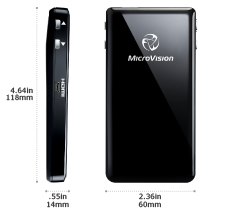
\includegraphics[scale=0.8]{measurements_showwx}
\end{center}
\vspace{-5mm}
\caption{Abmessungen des Microvision ShowWX+}
\label{fig.specs_proj}
\end{figure}

\clearpage{}

\section{Technische Spezifikationen des Arduino Nano}
\label{app:arduino}

\begin{table}[ht]
\caption{Technische Spezifikationen des Arduino Nano}
\begin{center}
\begin{tabular}{|l|r|}
\hline
\rowcolor{lightgray} \multicolumn{1}{|c|}{\textbf{Spezifikation}} & \multicolumn{1}{|c|}{\textbf{Wert}}\\
\hline
Microcontroller & Atmel ATmega328\\
\hline
Betriebsspannung & 5V\\
\hline
Eingangsspannung & 7-12V\\
\hline
Grenzen der Eingangsspannung & 6-20V\\
\hline
Digitale I/O Pins & 14\\
\hline
Analoge Eingangspins & 8\\
\hline
Gleichstrom pro I/O Pin & 40mA\\
\hline
Flash Speicher & 32KB\\
\hline
SRAM & 2KB \\
\hline
EEPROM & 1KB\\
\hline
Taktfrequenz & 16MHz\\
\hline
Länge & 45mm\\
\hline
Breite & 18mm\\
\hline
Gewicht & 5g\\
\hline
\end{tabular}
\end{center}
\label{tab:arduino}
\end{table}

\clearpage{}

\section{Technische Spezifikationen des Raspberry Pi}
\label{app:raspberry}

\begin{table}[ht]
\caption{Technische Spezifikationen des Raspberry Pi}
\begin{center}
\begin{tabular}{|l|r|}
\hline
\rowcolor{lightgray} \multicolumn{1}{|c|}{\textbf{Spezifikation}} & \multicolumn{1}{|c|}{\textbf{Wert}}\\
\hline
System-on-a-Chip & Broadcom BCM2835\\
\hline
CPU & 700MHz ARM11 ARM1176JZF-S\\
\hline
GPU & Broadcom VideoCore IV\\
\hline
Speicher & 512MB\\
\hline
USB 2.0 Ports & 2\\
\hline
Videoausgänge & Composite RCA, HDMI\\
\hline
Audioausgänge & 3,5mm Jack, HDMI\\
\hline
Low-Level Peripherie & 26 General Purpose Input/Output Pins,\\
& Serial Peripheral Bus Interface (SPI), I²C, I²S,\\
& Universal Asynchronous receiver/transmitter (UART)\\
\hline
Netzwerkschnittstelle & 10/100 wired Ethernet RJ45\\
\hline
Stromversorgung & 700mA\\
\hline
Spannungsversorgung & 5V\\
\hline
Länge & 85mm\\
\hline
Breite & 56mm\\
\hline
Höhe & 15mm\\
\hline
Gewicht & 31g\\
\hline
\end{tabular}
\end{center}
\label{tab:raspberry}
\end{table}

\clearpage{}

\section{Technische Spezifikationen des Microsoft Kinect Sensors}
\label{app:kinect}

\clearpage{}

\section{Bayes Filter}
\label{app:bayes}

\clearpage{}

\section{Konstruktionszeichnungen und Modelle}
\label{app:construction}

\clearpage{}

\section{Launchfiles}
\label{app:launchfiles}            % Anhang
    %\include{anhang_fehlerfortpflanzung}
		%\include{anhang_mgcEinstellungen}
		%\include{anhang_trafos}
		%\include{anhang_befestigen}
		%\include{anhang_datenblaetter}
  

    %% --- Anhang zu Ende
    \ihead{\normalfont\headmark}            % kolumnentitel innen
 
    

\end{spacing}
\end{document}                              % fertig!